%	Preamble
  \documentclass[12pt, letterpaper, oneside]{LaTeXConfig/Thesis} 
  \usepackage{setspace} % For picking line spacing *within* sections
  \usepackage{parskip} % For changing spacing between heads, lets me use linebreaks for spacing between paragraphs
  \usepackage{float}  % For Figures
    \floatstyle{plain} \restylefloat{figure} % Figures with Captions below
    \floatstyle{plaintop} \restylefloat{table} % Table with captions above
  % For Tables
    \usepackage{longtable} % For long tables that span many pages. | use \begin{longtable}
    \usepackage{booktabs}
  \usepackage[font={footnotesize}]{caption} % Make Fonts of Captions Small
  \usepackage{pdflscape} % Rotate page; BOTH printing and viewing! \begin{landscape} \end{landscape}
  \usepackage{helvet} \renewcommand{\familydefault}{\sfdefault} % Pick Ariel Font  
  \usepackage[T1]{fontenc}   % Standardize output fonts
  \usepackage{titlesec} % Center the Chapter and heading titles 
    \titleformat{\chapter}[display]
    {\normalfont\huge\bfseries\centering}{\chaptertitlename\ \thechapter}{20pt}{\Huge}
  \usepackage{flexisym} % Lets me use prime symbols
  \usepackage{gensymb} % For degree '\degree'
  \usepackage[square, comma, sort&compress]{natbib}  % For Referencing
    \setlength{\bibsep}{0.0pt} % Reduce size of bibliography
  \usepackage{bibentry} % For inserting Full Citation into preface
    \nobibliography* % Required to use the \usepackage(bibentry) above
  \usepackage{hyperref} % For internal referencing
    \hypersetup{urlcolor=blue, colorlinks=true}  % Colors hyperlinks in blue
  \usepackage{soul} % Highlight things use \hl{text}
  \usepackage[colorinlistoftodos]{todonotes} % To inserting Comments w/ \todo[prepend]{Comment text}
  \usepackage{changebar} % For putting bar in margin for review w/ \begin{changebar} & \end{changebar}
  \usepackage{listings} % For code inclusions
  \usepackage{color} % For code inclusions
    \definecolor{dkgreen}{rgb}{0,0.6,0} 
    \definecolor{gray}{rgb}{0.5,0.5,0.5}
    \definecolor{mauve}{rgb}{0.58,0,0.82}
    \lstset{
      frame=tb,
      language=Perl, % Change as needed locally w/ \lstset{language=LANG} where LANG=language of choice (i.e. PERL)
      aboveskip=3mm,belowskip=3mm,
      showstringspaces=false,columns=flexible,
      basicstyle={\footnotesize\ttfamily},
      numbers=none,
      numberstyle=\tiny\color{gray},
      keywordstyle=\color{blue},
      commentstyle=\color{dkgreen},
      stringstyle=\color{mauve},
      breaklines=true,breakatwhitespace=true
      tabsize=2}
  \usepackage{lipsum} % Generate Fill text w/ \lipsum[#] where #=paragraph num
  % Organism names
  \newcommand\flies{\textit{Drosophila melanogaster}}
  \newcommand\locusts{\textit{Schistocerca gregaria}}
  \newcommand\worms{\textit{Caenorhabditis elegans}}
% Gene names
  \newcommand\cd{\textit{CD45}}
  \newcommand\slo{\textit{slo1}}
  \newcommand\fn{\textit{Fn1}}
  \newcommand\kcnma{\textit{Kcnma}}
  \newcommand\dscam{\textit{Dscam1}}
  \newcommand\amyb{\textit{A-Myb}}
  \newcommand\bmyb{\textit{B-Myb}}
  \newcommand\cmyb{\textit{C-Myb}}
  \newcommand\miwi{\textit{Miwi}}
  \newcommand\mili{\textit{Mili}}
  \newcommand\spo{\textit{Spo11}}
  \newcommand\wdfy{\textit{wdfy3}}
  \newcommand\mybrepro{\textit{Mybl1}$^{repro9}$}
  \newcommand\dst{\textit{Dst1}}
 % Load macro/shortcuts for organism and gene names
  \title{\ttitle} % Defines the thesis title - don't touch this
  \begin{document}
\frontmatter % Use roman page numbering style (i, ii, iii, iv...) for the pre-content pages
  \setstretch{1} % Line spacing of 1
  % Define the page headers using the FancyHdr package and set up for one-sided printing
    \fancyhead{} % Clears all page headers and footers
    \rhead{\thepage} % Sets the right side header to show the page number
    \lhead{} % Clears the left side page header
    \pagestyle{fancy} % Finally, use the "fancy" page style to implement the FancyHdr headers  
  % PDF meta-data
    \hypersetup{pdftitle={\ttitle}}
  	\hypersetup{pdfsubject=\subjectname}
  	\hypersetup{pdfauthor=\authornames}
  	\hypersetup{pdfkeywords=\keywordnames}
  %----------------------------------------------------------------------------------------
%	TITLE PAGE Umass
%----------------------------------------------------------------------------------------
\begin{titlepage}
\begin{center}
	\huge \ttitle \\[2cm] 
	{\large 
		A Dissertation Presented \\[1cm]
		By \\[1cm]
		Christian K. Roy \\[1cm]
		Submitted to the Faculty of the University of the \\
		Massachusetts Graduate School of Biomedical Sciences, Worcester\\
		in partial filfillment of the requirements\\
		for the degree of \\[2cm]
		DOCTOR OF PHILOSOPHY \\[1cm]
		MAY 21st 2014\\[1cm]
		BIOCHEMISTRY\\[1cm]
 	}
 \end{center}
 \end{titlepage}
 
  %----------------------------------------------------------------------------------------
%	Signature Page Umass
%----------------------------------------------------------------------------------------
\begin{titlepage}\label{hd:titlePage}
\begin{center}
		\ttitle \\[0.25cm]

		A Dissertation Presented \\[0.25cm]
		By \\[0.25cm]
		Christian K. Roy \\[0.25cm]
 
		The signatures of the Dissertation Defense Committee signify \\
		completion and approval as to style and content of the Dissertation\\[1cm]
		\rule[1em]{25em}{1pt}\\[-0.6cm]% This prints a line for the signature
		Melissa J. Moore, Co-Thesis Advisor\\[1cm]
		\rule[1em]{25em}{1pt}\\[-0.6cm]
		Phillip D. Zamore, Co-Thesis Advisor\\[1cm]
		\rule[1em]{25em}{1pt}\\[-0.6cm]
		Job Dekker, Member of Committee\\[1cm]
		\rule[1em]{25em}{1pt}\\[-0.6cm]
		Brenton R. Graveley, Member of Committee\\[1cm]
		\rule[1em]{25em}{1pt}\\[-0.6cm]
		Scot A. Wolfe, Member of Committee\\[1cm]
		The signature of the Chair of the Committee signifies that the written
		dissertation meets the requirements of the Dissertation Committee\\[1cm]
		\rule[1em]{25em}{1pt}\\[-0.6cm]
		Zhiping Weng, Chair of Committee\\[0.25cm]
		The signature of the Dean of the Graduate School of Biomedical Sciences signifies that the student has met all graduation requirements of the school.\\[1cm]
		\rule[1em]{25em}{1pt}\\[-0.6cm]
		Anthony Carruthers, Ph.D.,\\[0.25cm]
		Dean of the Graduate School of Biomedical Sciences\\[0.25cm]
		Biochemistry and Molecular Pharmacology\\[0.25cm]
		MAY 21st 2014 

 \end{center}
 \end{titlepage}
\clearpage % Start a new page

  % !TEX root = /Users/royc/Google_Drive/Thesis/RoyC_Umass_Thesis.tex
\addtotoc{Abstract} % Add the "Abstract" page entry to the Contents
\label{hd:abstract}
\abstract{}

Analysis of gene expression has undergone a technological revolution. What was impossible 6 years ago is now routine. High-throughput DNA sequencing machines capable of generating hundreds of millions of reads allow, indeed force, a major revision toward the study of the genome's functional output---the transcriptome. This thesis examines the history of DNA sequencing, measurement of gene expression by sequencing, isoform complexity driven by alternative splicing and mammalian piRNA precursor biogenesis. Examination of these topics is framed around development of a novel RNA-templated DNA-DNA ligation assay (SeqZip) that allows for efficient analysis of abundant, complex, and functional long RNAs. The discussion focuses on the future of transcriptome analysis, development and applications of SeqZip, and challenges presented to biomedical researchers by extremely large and rich datasets.

\setcounter{page}{3}
\clearpage % Start a new page
  % !TEX root = /Users/royc/Google_Drive/Thesis/RoyC_Umass_Thesis.tex
\setstretch{1} 
\acknowledgements{}\label{hd:acknowledgements}

First I would like to thank Laura Geagan and Rebecca Sendak, my supervisors while a research associate at Genzyme. Without the confidence they instilled in my abilities as a young researcher I doubt I would have ever signed up for more school.

During my 1st year retreat at Wood’s Hole I observed Melissa's fantastic ability as a communicator of interesting and important Science. She brought out her rope representing unspliced dystrophin---a rope that reached to the back of a rather large auditorium---and then dramatically held up a ``No.2'' pencil representing the final mRNA product. Both were to scale. I knew then that I wanted join her lab. Thanks Melissa for teaching me so much.

Soon after joining Melissa’s lab, with a project going well, it was proposed that I be a joint student between Melissa and Phil. It was not difficult to jump at the opportunity to be advised by \textit{two} Hughes Investigators. I have been continually amazed at the depth of Phil’s knowledge. He is a careful, meticulous, quantitative, and careful mentor. Phil forces me to think and act outside my comfort zone, something I always tell myself is essential for change and growth. Thank you Phil for everything I've learned.

My committee has also been very supportive throughout my PhD. I hardly believed the ease with which I passed my qualifying exam and figured there must have been some mistake. TRAC meetings confirmed that I was not thinking off-base. One-on-one meetings just prior to my QE were especially helpful. Thanks to Scot, Job, and Zhiping for all your guidance.

Thanks to all members of the Za(Moore) labs, past and present. Specifically I would like to thank other members of my year in the Moore Lab, Eric and Erin. Thanks to fantastic past post-docs Amrit, Alper, and Aaron. Also thanks again to Alper and to Bo and Can for my novice bioinformatic questions.

Thanks to the faculty I have interacted with throughout my time at Umass, including Dave Weaver, Brent Graveley, Andres Muro, Manuel Garber, and Heinrich Gottlinger. And thanks to Anna from the Gottlinger lab for involving me in her HIV and hUPF1 story.

My project was pushed forward by a pair of great rotation students: Ben Landry and Ogooluwa (``Ogo'') Adegoke Ojelabi . Thanks you two for letting me know SeqZip was robust beyond my own hands.

My family always instilled the importance and value of education. Thank you Mom, Dad, Grandpa and Grandma for sacrificing to provide me so much opportunity. I hope I have made you proud.

Finally, and most importantly, I would like to acknowledge the love and support of my wife, Julie. Much of my success can be attributed to her hard work and support over the last 15 years. Our son, Owen, is lucky to have such an amazing mom. Our family is truly blessed. Thanks P :)

\clearpage % Start a new page
  % !TEX root = /Users/royc/Google_Drive/Thesis/RoyC_Umass_Thesis.tex
%----------------------------------------------------------------------------------------
\pagestyle{fancy} 
\lhead{\emph{Contents}} % Set the left side page header to "Contents"
\setcounter{tocdepth}{2}  % Limits to print UP TO AND INCLUDING \subsection 
\tableofcontents % Write out the Table of Contents
\lhead{\emph{List of Figures}} % Set the left side page header to "List of Figures"
	\listoffigures % Write out the List of Figures
\lhead{\emph{List of Tables}} % Set the left side page header to "List of Tables"
	\listoftables % Write out the List of Tables
% Comment this out before final run
%\lhead{\emph{List of Todos!}} % Set the left side page header to 'List of Tables"
%  \listoftodos % Write out the List of Todos
%  \todototoc
  \clearpage % Start a new page
\setstretch{1.5} % Set the line spacing to 1.5, this makes the following tables easier to read
\lhead{\emph{List of Abbreviations}}
\listAbbreviations
\begin{table}[h]
  \label{hd:abrevs} 
  \begin{tabular}{l|l}
  AS       & Alternative Splicing                                 \\
  DNA      & Deoxyribonucleic acid                                \\
  ssDNA    & Single-stranded DNA                                  \\
  RNA      & Ribonucleic acid                                     \\
  ssRNA    & Single-stranded RNA                                  \\
  ATP      & Adenosine triphosphate                               \\
  NAD      & Nicotinamide adenine dinucleotide                    \\
  ChIP-Seq & Chromatin Immunoprecipitation followed by sequencing \\
  EST      & Expressed Sequence Tag								\\
  HTS      & High-throughput sequencing (see also NGS)            \\
  NGS      & Next-generation sequencing                           \\
  CAP      & 5\textprime~ 7meG structure attached to mRNAs        \\
  nt       & A nucleotide of either DNA or RNA                    \\
  bp       & A base pair of DNA                                   \\
  SRE      & Splicing Regulatory Element                          \\
  IRE      & Intron Recognition Element                           \\
  CNS      & Central Nervous System                               \\
  TSS      & \{Transcription or Translation\} Start Site          \\
  TTS      & \{Transcription or Translation\} Termination Site    \\
  SAGE     & Serial Analysis of Gene Expression                   \\
  hnRNP    & heterogeneous nuclear ribonucleoprotein              \\
  FISH     & Fluorescence in situ hybridization                   \\
  GFP      & Green Fluorescencent Protein                         \\
  MPSS     & Massively Parallel Signature sequencing              \\
  \end{tabular}
  \end{table}
\clearpage
  %----------------------------------------------------------------------------------------
%	SYMBOLS
%----------------------------------------------------------------------------------------
\clearpage % Start a new page
\lhead{\emph{List of Symbols}}
\label{hd:Symbols} \listSymbols

\begin{table}[h]
\begin{tabular}{ll}
5\textprime       & The 5 prime end of a DNA or RNA molecule 			\\
3\textprime       & The 5 prime end of a DNA or RNA molecule 			\\
$\mu$       	  & Micro. A value of 1x10\textsuperscript{-6} standard units 			\\
\end{tabular}
\end{table}
  % !TEX root = /Users/royc/Google_Drive/Thesis/RoyC_Umass_Thesis.tex
\lhead{\emph{Definitions}}
\label{hd:Definitions} \listDefinitions

\begin{description}
  \item[RNA-Seq]
  A technology wherein RNA is fragmented, converted to DNA, and analyzed on a high-throughput sequencing instrument

  \item[A ``Read'']
  The sequence of nucleotides produced from each spot on a high-throughput sequencing machine

  \item[Insert]
  The RNA molecule captured between two cloning sequences in a high-throughput sequencing library preparation workflow

  \item[Read length]
  The number of nucleotides for each given ``read''

  \item[Read depth]
  The number of reads obtained from each high-throughput sequencing analysis

  \item[Coverage]
  A measure of the number of times each nt of a genome is sequenced. E.g. 100 million reads of a 10 million nt genome = 10X coverage, assuming uniform distribution of the ``reads''

  \item[Paired-end]
  When both sides of a DNA insert or template are sequenced, utilizing the original length of DNA between the reads to facilitate mapping (\cite{Roach1995}).

  \item[Scaffold or Contig]
  A draft sequence of nucleotides, meant to represent the actual biological sequence as closely as possible, examples include unassembled fragments of chromosomes or fragments of mRNA transcripts.

  \item[Argonaute]
  Protein(s) belonging to a group containing a Piwi (P-element induced wimpy testes) domain, that bind nucleic acids and participate in many target-guided processes, including RNA Interference, and RNA-induced transcript/gene silencing.

  \item[Ligamer]
  A DNA oligonucleotide containing two distinct regions of complementarity to a 5\textprime~ and 3\textprime~ section of RNA. Each region is normalized for $^{Tm}$ such that the length of each section is \textasciitilde15--30 nt. These two regions are connected by a short sequence of the designer's choice, usually >5 nt in length. Each ligamers overall length is \textasciitilde45\textendash 60 nt. See figures \ref{SeqZipMethod:fig:Original SeqZip Diagram} and \ref{SeqZipPaper:fig:Roy2014 F1}.
  
  \end{description}
  \clearpage % Start a new page
  \setstretch{1.3} % Return the line spacing back to 1.3
\pagestyle{empty} % Page style needs to be empty for this page
%\addtocontents{toc}
\label{hd:Dedicatory}
\dedicatory{
	I would like to dedicate this Doctoral dissertation to my grandfather, George Knauf. My grandfather passed away on September 23rd, 2011, just one week shy of his 82nd birthday. I find it difficult to articulate how much I miss him. He spoke carefully and never without purpose or conviction. While I hear from others that he was proud of me, he rarely, if ever, betrayed that type of emotion directly. It is my goal to build as solid a life as he, founded on hard work, playing the long game, responsibility, and maintaining friendships. These are just a few of the personality traits that I observed and try to emulate. The fact that he passed before he could meet our son Owen is one of my biggest regrets. Of all the possessions he left behind, it is the memory of our time together that I will cherish the most. Rest in peace, Grump. I did it. 
} % Dedication text
\clearpage % Start a new page
  %----------------------------------------------------------------------------------------
%	Preface
\prefaceSection{}

The work reported in this dissertation has been published in the following articles.
Chapter \ref{Chapter4} has been published previously as:\\
Li, X. Z. Z., Roy, C. K. K., Dong, X., Bolcun-Filas, E., Wang, J., Han, B. W. W., … Zamore, P. D. D. (2013). An Ancient Transcription Factor Initiates the Burst of piRNA Production during Early Meiosis in Mouse Testes. Molecular Cell, 50(1), 1–15. doi:10.1016/j.molcel.2013.02.016

Some contents of Chapter \ref{Chapter3} are included in a currently submitted manuscript. 

\clearpage
\mainmatter % Begin numeric (1,2,3...) page numbering
  \pagestyle{fancy} % Return the page headers back to the "fancy" style
  %\setstretch{2} % Line spacing of 2
  \setstretch{1} % Line spacing of 1
  \label{hd:Chapters}
  % !TEX root = /Users/royc/Google_Drive/Thesis/RoyC_Umass_Thesis.tex
\chapter{Introduction}  \label{Intro} 
\lhead{Chapter 1. \emph{Introduction}} 
%----------------------------------------------------------------------------------------

\section{Fixed Genomes and Flexible Genes}
  \label{Intro:sec:Fixed Genomes and Flexible Genes} 

  Exodus tells of the liberation of the Israelites from Egyptian slavery. Humble and reluctant Moses, their divine-appointed messiah, attempts to force the Pharaoh Ramses to release the Israelites through inflicting 10 plagues. Pharaoh is stalwart and stubborn as water turns to blood and the streets are flooded with frogs, lice, and flies. As livestock falls dead from disease, people and animals both are covered in boils, and the land burns in storms of fire, Pharaoh does not bend.

  The 8th plague was a swarm of Locusts, described in Exodus 10: 14-15:

  \begin{quote}
    \itshape
    \singlespacing
    \textsuperscript{14} And the locusts went up over all the land of Egypt, and rested in all the coasts of Egypt: very grievous were they; before them there were no such locusts as they, neither after them shall be such.\\ 
      \\
    \textsuperscript{15} For they covered the face of the whole earth, so that the land was darkened; and they did eat every herb of the land, and all the fruit of the trees which the hail had left: and there remained not any green thing in the trees, or in the herbs of the field, through all the land of Egypt.
    \end{quote}

  The desolation of a locust plague was still not enough to persuade Ramses. Nor was three days of darkness. Only after the death of all first-born Egyptians, including Ramses own son, was Pharaoh persuaded to liberate the Israelites.

  Locust swarms are not biblical fantasy. Today the United Nations' Food and Agriculture division maintains a \href{http://www.fao.org/ag/locusts/en/info/info/news/index.html}{Locust watch website} that provides weekly updates on potential swarms in northern Africa and the Middle East. Locusts have long been, and continue to be, a powerful and feared force of Nature.

  Unlike fire and brimstone, locusts are something that can be observed and studied. What triggers a swarm? We know that the desert locust, \locusts{}, is the one of 10 species that swarm and cause massive crop damage. \locusts{} are in the insect Order Orthoptera, along with crickets and katydids. Orthoptern members make sounds known as \textit{stridulation} by vigorously rubbing their wings, making for a noisy cloud of devastation. They only weigh 0.05--0.07 ounces and are less than 2.5 inches long but can consume their own body weight in vegetation per day. One \href{http://animaldiversity.ummz.umich.edu/site/accounts/information/Melanoplus_spretus.html}{swarm} of the infamous, and now curiously extinct, Rocky Mountain locust contained 12.2 \textit{trillion} insects. Its estimated total weight was 27.5 \textit{million} tons. The swarm covered almost 200 square miles (2/3 the size of Manhattan), and could travel 60 miles in a day. A locust swarm is truly a modern biblical plague.

  \begin{figure} % Desert Locus Figure
    \centering 
    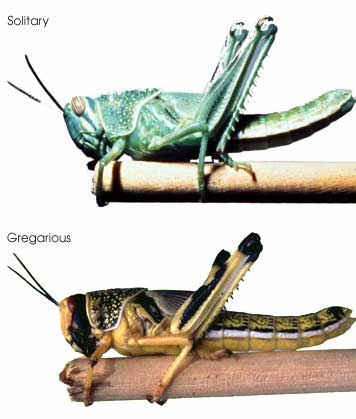
\includegraphics[width=10cm,keepaspectratio]{Figures/Intro/DesertLocust.jpeg}
    \caption[The Solitary and Gregarious forms of \locusts{}]
    {
      The Solitary and Gregarious forms of \locusts{}\\[0.25cm]
      The two phenotypic forms of \locusts{} appear very different. The solitary form is green and generally larger, while its gregarious form is more brightly colored, smaller, and swarms in vast numbers. Photo from \href{http://www.wikicommons.com}{Wikicommons}.
      }
    \label{Intro:fig:Locust}
    \end{figure}

  By definition swarms are temporary; the movement, en masse, from one location to another. But where do 12.2 trillion locusts go when not swarming? Does anyone care if their crops aren't under assault? It seemed no one cared until 1921 when an important realization was made.

  The power and destruction \locusts{} can inflict makes it difficult to believe that they are nothing more than common grasshoppers. Nothing more than grasshoppers not just by analogy, but by actual \textit{Taxonomy}. ``Desert'' locusts are actually the \textit{gregarious} form  of \locusts{} (Figure \ref{Intro:fig:Locust}), while the more familiar and docile looking ``grasshopper'' is the \textit{solitary form}. How does such a dichotomy exist within the same organism---indeed the same \textit{genome}?

  \locusts{} are \textit{polyphenic}, meaning that they have multiple (poly) physical forms (phenotypes). Polyphenism is a general feature among insects. These phenotypes are often extremely different. For example, pea aphids (\textit{Acyrthosiphon pisum}), which usually exist in an asexually reproducing, wingless female form, respond to reduced food supply and overcrowding by producing winged sexually-reproducing offspring. Winged organisms travel to new sources of food and revert back to the asexually reproducing form \citep{Shingleton2003,Purandare2014b}. In the case of \locusts{}, the gregarious form is smaller and more brightly colored compared to its solitary cousins. This transformation can happen in as little as two hours. What is the underlying cause of this transformation?

  In 2009, \citet{Anstey2009} reported that after two hours of forced crowding \locusts{} displayed elevated levels of the neurotransmitter serotonin in the ganglia (brain). Serotonin levels were strongly correlated with other gregarious form indicators. Serotonin regulates neuronal junctions and wiring in the brain \citep{Hoeffer2003}. Through the integration of environmental and social cues, the grasshopper brain can be re-wired, resulting in tremendous changes in behavior and phenotype. These changes prepare the organism to deal with a different world. It allows the organism to survive. Survival that is to the detriment of surrounding agriculture.

  In an extremely interesting \href{http://aeon.co/magazine/nature-and-cosmos/why-its-time-to-lay-the-selfish-gene-to-rest/}{article}, David Dobbs compares the two forms of \locusts{} to that of Dr. Jekyll and Mr. Hyde, the principle characters in the Robert Louis Stevenson novella. For Dr. Jekyll in fiction, and for \locusts{} in reality, the power to morph into multiple forms demonstrates the incredible power of a fixed genome yet plastic gene expression. 

  It is often said that something is ``in the genes.'' Another oft-heard idiom that is perhaps more appropriate is: ``it's how you use them.'' This thesis will illustrate that, with ever increasing resolution in the measurement of functional gene products (i.e. the ``transcriptome''), we are beginning to realize the tremendous diversity and complexity of gene expression.

\section{Nucleic Acid Sequencing}
  \label{Intro:sec:Nucleic Acid Sequencing}

  \subsection{DNA Sequencing}
    \label{Intro:subsec:DNA Sequencing History}

    That DNA is the source of genetic information in all living organisms was first realized in 1953 \citep{Watson1953a}. The \textit{``pretty''} and \textit{``elegant''} arrangement of complementary, antiparallel, DNA strands captivated everyone, including one of DNAs co-discoverers \citep{Watson2012a}. Yet it took 25 years after the structure was known to be able to determine specific arrangements of nucleotide bases in a given length of DNA (i.e. to ``sequence''). By 1977, two completely different methods developed by Sanger \citep{Sanger1975a,Sanger1977b} and Maxam-Gilbert \citep{Maxam1977a} were reported. These sequencing technologies, from then on referred to eponymously as ``Sanger'' or ``Maxam-Gilbert'' sequencing, were used to determine the specific order of a small piece of DNA (200--300 nt). Over the next 35 years, DNA sequences were slowly cloned, sequenced, analyzed, and dutifully cataloged into knowledge.

    During the late 1970's and throughout the 1980's, DNA sequences were typically communicated in important publications \citep{Cordell1980a,Sanger1978a}. The birth of the Internet in the 1990's allowed publicly-funded repositories to store sequence information \citep{Benson2011a}. Yet it took the human genome project to transform tedious and balkanized DNA sequencing efforts into an organized process capable of assembling complex genomes \citep{Lander2011a,Venter2001}. An often criticized, but undeniably disrupting force in the human genome project was the competing efforts by the privately-owned company Celera \citep{Venter2008a}. Instead of assigning specific sections of the genome to be worked out by individual labs, Celera centralized the efforts by collecting many of the best ``high-throughput'' Sanger-sequencing devices from Agilent (ABI 3700 DNA Analyzer). Celera used a ``shotgun'' sequencing approach \citep{Staden1979}, combined with sequence scaffolds from the publicly-funded project, to quickly assemble a high-quality genome. Arguably, this was the first deep sequencing effort. Coincident with the beginning of a new millennium. It changed the landscape of molecular and biochemical research.

  \subsection{High-throughput Sequencing}
    \label{Intro:subsec: History of HTS}

    Sanger's DNA sequencing technology remains a valuable tool for every biological scientist. However, Sanger sequencing has a practical throughput limit. Each DNA molecule to be sequenced must be isolated, cloned, and amplified---using bacteria. Given that the human genome \citep{Hattori2005a} comprises >3 billion bp, and each Sanger reaction provides \textasciitilde800 nt of quality sequence, at least \textasciitilde4 million individual reactions are needed to determine the sequence of the human genome. This number assumes all ``reads'' are of sufficient quality, length, and do not overlap by even 1 nt.

    Even the best practical improvements to Sanger work-flows could not bring the technology in-line with aspirations of analyzing many species and/or organisms. The early 2000's saw multiple efforts to improve the scale of DNA sequencing, first using Massively Parallel Signature sequencing (MPSS) \citep{Brenner2000a}, but perhaps more importantly, by Pyro- \citep{Ronaghi1998a} and Polony-sequencing \citep{Shendure2005}. Both pyro- and polony sequencing use emulsion PCR \citep{Nakano2003a} for clonal amplification prior to sequencing, removing the bottleneck of bacterial cloning. In contrast to Sanger sequencing, where fluorescence signal from the last incorporated chain-terminating nucleotide is observed, pyrosequencing visualizes light given off by luciferase reacting with pyrophosphate (PPi), a by-product of nucleotide incorporation. This approach was later commercialized by 454 technologies. Polony sequencing involves a sequencing-by-ligation method, eventually commercialized by Applied BioSystems and branded as SOLiD sequencing. 
    % ER Comment: Suggests figure showing how these two technologies work
    While both of these technologies provided valuable high-throughput sequences, neither has been as successful as the approach commercialized by Solexa, now known as Illumina.

    Illumina sequencers use a sequencing-by-synthesis approach. After clonal amplification of DNA on a slide surface \citep{Bentley2008}, fluorescent nucleotides are visualized as they are incorporated into the growing DNA strand. Iterations of the Illumina platform (e.g. GE, GE-II(x), HiSeq, HiSeq 2500, Hi X) have demonstrated steady and impressive increases in both read depth and length. On February 15th 2012, Illumina announced on its \href{http://blog.basespace.illumina.com/}{Basespace blog}, that they had sequenced a haplotype map (HapMap) sample at 40X coverage, using the HiSeq 2500 platform and paired-end 100 nt reads in a single run. On January 14th, 2014, Illumina \href{http://bit.ly/PZpegZ}{announced} its HiSeq X system, the first platform to truly attain the benchmark \$1,000 genome \citep{Service2006,Hayden2014}. These machines demonstrate that sequencing genomes is no longer the monumental endeavor it once was and that completely new experimental possibilities are a reality for life science researchers (Figure \ref{Intro:fig:SeqCosts}).

    \begin{figure} % Sequence Costs over time
      \centering 
      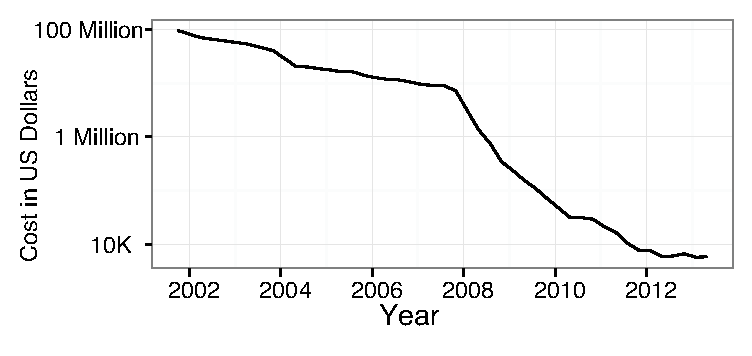
\includegraphics{Figures/Intro/Sequencing_costs_over_time.eps}
      \caption[Cost of sequencing the human genome over time]
      {
        Cost of sequencing the human genome over time\\[0.25cm]
        The costs of sequencing the human genome has decreased on a log scale over a 10 year period due to major improvements in high-throughput sequencing. Data from Wetterstrand KA. DNA Sequencing Costs: Data from the NHGRI Genome Sequencing Program (GSP) Available at: \url{www.genome.gov/sequencingcosts}. Accessed 2014-05-04).
        }
      \label{Intro:fig:SeqCosts}
      \end{figure}

  \subsection{RNA Sequencing}
    \label{Intro:subsec:Types of HTS}

    The first widely-accepted large scale method used to measure gene expression was Serial Analysis of Gene Expression (SAGE) \citep{Velculescu1995a}. SAGE, like the before mentioned MPSS technique, produces a digital output of gene expression using a clever procedure of restriction endonucleolytic cDNA cleavage. Cleaved-product sticky ends are concatenated together to form long DNA fragments. 
    % ER Comment: Suggests SAGE figure showing how it works
    Fragments are cloned into a vector, amplified, and Sanger sequenced. Using known sequences incorporated during concatenation, the number of sequenced fragments that align to a given gene is related to the abundance of the original RNA molecule. A clever molecular trick, SAGE allowed researchers to dip into the 5-log range of mRNA expression. However, the technique is still limited by Sanger sequencing read lengths and depth.

    After SAGE but prior to second generation high-throughput sequencing (HTS) technology, microarrays were the goto approach for gene expression analysis. The importance of microarrays in the measurement of gene expression cannot be overstated \citep{Shendure2008,Marioni2008}. However, limitations of novel sequence discovery combined with analogue signal, make the relevance of microarray technology limited in application to complete isoform discovery and annotation (see Section\ref{Intro:sec:Isoform Problem} and Figure \ref{Intro:fig:NoConnectivityInHTSMethods}). Yet Microarray technology is still very relevant. For example, use of microarrays in the recent definition of the developing human brain transcriptome---where sample was precious and quantification of known genes was of more importance than novel isoform discovery--was a prudent analysis platform choice \cite{Miller2014}.

    Different from SAGE and microarrays, the Solexa/Illumina platform relies on clonal amplification of a single template directly on a slide surface and is therefore not restricted by bacterial cloning. This new form of ``massively parrallel'' amplification uses imaging of clonal cDNA spots with sensitive digital cameras during sequential addition of fluorescent nucleotides (\textit{sequencing by synthesis}). Machines from Illumina turned out to posses the right mix for a ``second generation'' HTS platform. Soon after the Solexa/Illumina platform achieved read lengths of sufficient length and depth to measure gene expression, the first RNA-Seq papers were published \citep{Mortazavi2008, Nagalakshmi2008,Lister2008}, providing a glimpse into the future of molecular biology. Indeed, in the years since, analysis by RNA-Seq has quickly overtaken other forms of gene expression analysis, as demonstrated by the number of accessions created in the publically-funded repository of sequencing data, the Gene Expression OmniBus (GEO) \citep{Barrett2013}. RNA-Seq allows for digital quantification of RNA expression across more physiologically-relevant ranges \citep{Blencowe2009}, novel sequence discovery, measuring RNA-editing \citep{Li2011}, and fuels the novel area of transcript assembly \citep{Trapnell2010}. Through modification of the basic protocol or performing additional biochemical steps, RNA-Seq can be used to investigate many aspects of RNA biology (Figure \ref{Intro:fig:htsMethods} and \citep{Mutz2013}).

    \begin{figure} % RNA Sequencing Methodologies
      \centering 
      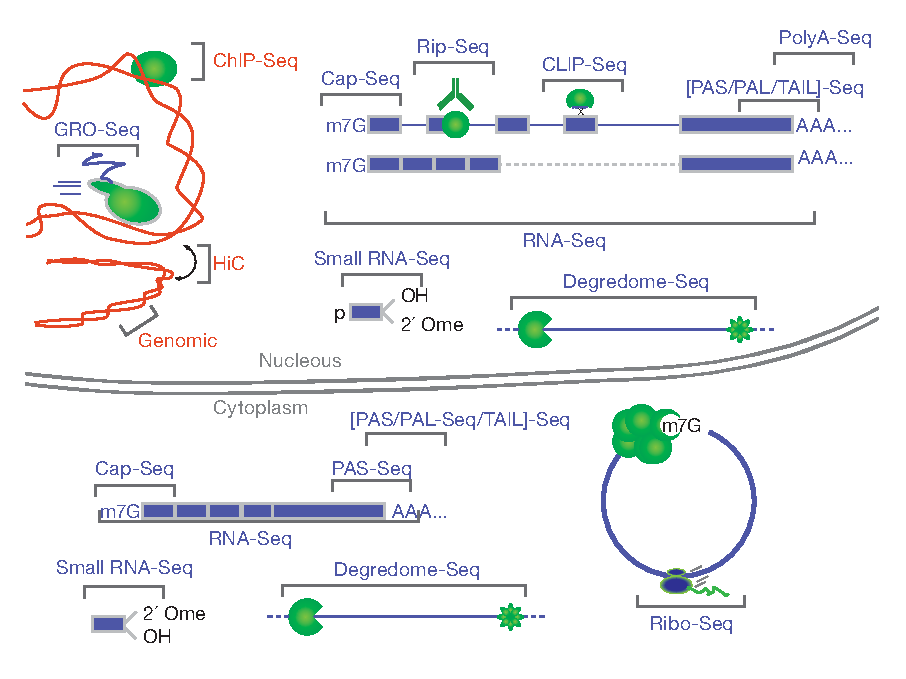
\includegraphics{Figures/Intro/RNA_Sequencing_methodologies.eps}
      \caption[Methods for High-throughput sequencing of RNA]
      {
      Methods for High-throughput sequencing of RNA\\[0.25cm]
      In the short years since the first report of RNA-Seq, many variations have been reported. The figure above provides an incomplete graphical illustration of these variations. A more complete list of ``*Seq'' applications is maintained on this \href{http://liorpachter.wordpress.com/seq/}{blog} \url{http://liorpachter.wordpress.com/seq}.
      }
      \label{Intro:fig:htsMethods}
      \end{figure}

    Numerous methodologies enrich RNA-Seq libraries for particular types of RNA. For example, measurement of nascent transcripts can be performed via Global Nuclear Run-on sequencing (GRO-Seq) \citep{Core2008a}, and the extremely complicated process of RNA turnover (referring to the rates at which RNAs both are produced and degraded) has been examined \citep{Ghosh2010a, Tani2012}. RNA::Protein interactions can be measured with or without cross-linking the protein to the RNA, via CLIP or RIP, respectively (see section \ref{Disc:subsec:Labeling of precursors}) \citep{Ule2005,Licatalosi2006,Singh2013}. Once an RNA has been fully transcribed, known processing steps such as 5\textprime~7meG CAP formation and poly(A)+ tail formation can be measured using any of the Cap-Seq/CAGE \citep{Shiraki2003a} or PAS/TAIL/PAL methodologies \citep{Shepard2011, Chang2014b, Subtelny2014}. Importantly, nascent RNA can also be captured via Cap-Seq \citep{Kruesi2013}. With appropriate size-selection steps, small RNAs \citep{Ghildiyal2008} can also be captured. Finally, traditional RNA-Seq can capture many of the same RNA fragments as the above mentioned methods, even though it is mainly associated with measurement of traditional mRNA.

    RNA-Seq (and all its flavors) are traditionally associated with quantification of RNA obtained from \textit{many} tissue culture cells or bulk pieces of tissue. Recently, efforts to measure RNA expression in a single cell has gained attention \citep{Shapiro2013b}. Perhaps the most interesting concept concerning single-cell gene expression is the ``biological uncertainty principle'', wherein it is possible to either know, or change --- but not both---~the RNA composition of a single cell. The name borrows from Heisenberg's uncertainty principle \citep{Kennard1927} and is often confused with the more appropriate ``Observer effect'' \citep{Riley2013}. Leaving that issue aside, measuring the unique transcriptome of a cell is surely an exciting and informative endeavor \citep{Marinov2013, Shalek2013b,Wills2013}. Compared to DNA, the diversity of RNA synthesis within living cells is more complicated \citep{Shendure2012} and the ability to accurately measure RNA dynamics among cells should allow for more informative observations concerning biology than is currently possible using bulk measurements.
    %MO Comment : "This last PP feels a little mis-placed or irrelevant - I think you want to talk about the future of RNA Seq and single-cell is definitely futuristic. I'd kill the uncertainty principle and would rather hear what I can learn from single-cell that I can't from bulk, and what are some of the barriers to further adoption of this method - what are the current limits of single-cell RNASeq which need to be overcome?"

\section{Nucleic Acid Splicing}
  \label{Intro:sec:Nucleic Acid Splicing}

  1977 brought the discovery of ``split genes'' \citep{Berget1977,Chow1977}. Almost immediately it was reasoned that RNA transcribed from split genes could be arranged in different combinations, greatly increasing the coding potential of a genome \citep{Gilbert1978a}. Differential arrangement of gene products via transcription and splicing, where at least two unique transcripts produced, known as \textit{alternative splicing}, has proven to be an integral part of eukaryotic gene expression.

  \subsection{Alternative Splicing}
    \label{Intro:subsec:Alternative Splicing}

    The number of genes estimated to be alternatively spliced has grown considerably. In 1993, Phillip Sharp, Co-Nobel-prize winner for the discovery of splicing, stated that: ``Approximately, one of every twenty genes is expressed by alternative pathways of RNA splicing in different cell types or growth states'' \cite{Sharp2014}. Not long after the assembly of the first human genome, a number of groups combed through Expressed Sequence Tag (EST) databases to increase that estimate to 35\%-59\% \citep{Modrek2002}. Soon after, analysis using specially designed ``splicing sensitive'' microarrays resulted in an increased estimate of 74\% \citep{Johnson2003}. In late 2008, three groups used RNA-Seq to demonstrate that between 86\% and 95\% of human multi-exon genes are subject to alternative splicing \citep{Pan2008, Wang2008, Sultan2008}. Not only did they demonstrate that almost all genes are alternatively spliced, they also showed that alternative splicing often occurs in a tissue- and cell type-specific manner. In combination with transcription regulation, the study of alternative splicing is critical to advance our understanding how comparably static genomic DNA sequence produce the highly flexible and adaptive transcriptomes of organisms.

    A pair of papers recently published in Science best illustrate the amazing complexity alternative splicing can generate between, and perhaps more importantly \textit{within}, organisms \citep{Barbosa-Morais2012,Merkin2012}. RNA-Seq performed on a diverse array of organisms and tissues has revealed that splicing patterns are shared more closely between organs of different species than between different organs within a species. Alternative splicing is essential for physiologically-specialized organs to use a common genome.

    \begin{figure} % # of Genes and % Alternatively Spliced
      \centering 
      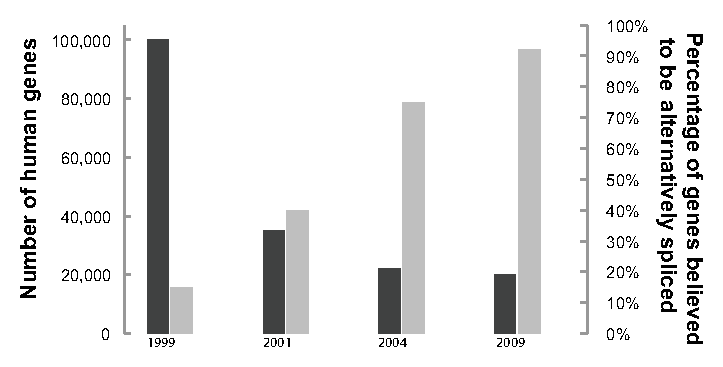
\includegraphics{Figures/Intro/numberHumanGenesAndNumberSpliced}
      \caption[Estimates of number of human genes, and percentage alternatively spliced over time]
      {
      Dark Grey - Estimates of number of human genes; Light Grey - Estimates of what percent of genes undergo some form of alternative splicing.
      }
      \label{Intro:fig:numGenesAndNumSpliced}
      \end{figure}

    Alternative splicing is an essential regulatory mechanism involved in the control of gene expression. Its combinatorial nature could potentially answer many basic questions concerning gene expression, such as a physical explanation of what separates us from our closest evolutionary ancestor, the chimpanzee \citep{Calarco2007a}. Additionally, the influence of alternative splicing on disease and cancer is slowly coming to light \citep{Tazi2009}. Unfortunately, because of the limitations of methods currently used for the large-scale analysis of isoform expression, we fail to obtain the complete picture of alternative splicing. One specific missing element of that picture is the prevalence of coordination between different regions of alternative splicing separated by large spans of sequence. An efficient, large-scale, single-molecule technique that maintains isoform sequence connectivity is required to complete the complicated picture of alternative splicing.

  \subsection{The Connectivity Problem}
    \label{Intro:sec:Isoform Problem}

    Alternative splicing research now relies on large-scale (aka: \textit{global}, \textit{genome-wide}, \textit{high-throughput}) techniques. Two of the most widely-applied technologies employed for large-scale analysis of gene expression are microarrays and ``2nd generation'' HTS. Unfortunately, both of these techniques have fundamental limitations, with the major issues being probe specificity for the former and read length for the latter.

    \begin{figure} % Seqlengths and Connectivity
      \centering 
      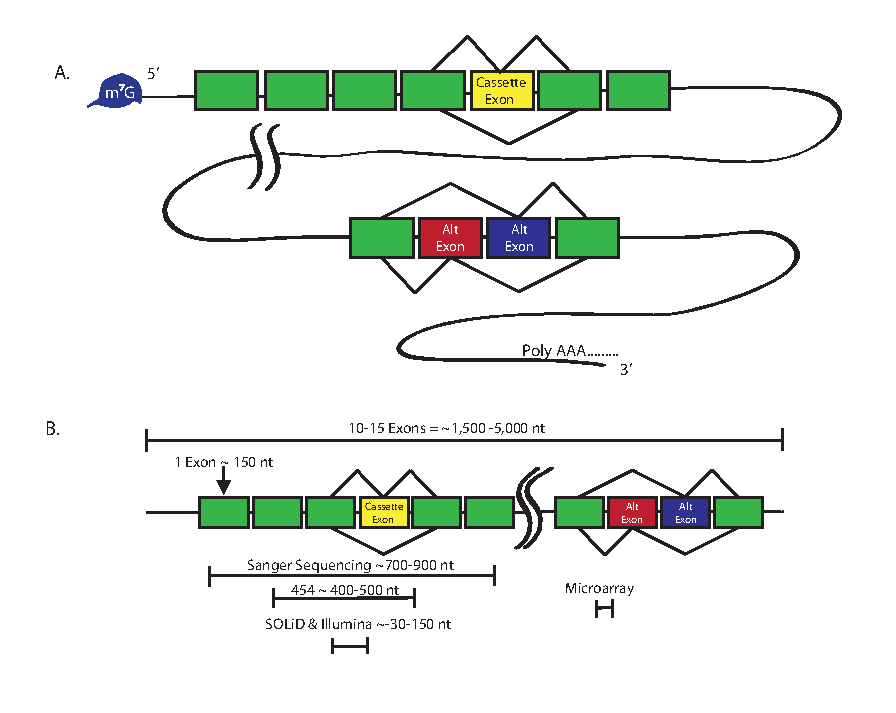
\includegraphics{Figures/Intro/SeqLengths_and_Connectivity.eps}
      \caption[HTS read lengths are not sufficient to maintain alternative splicing connectivity]
      {
        HTS read lengths are not sufficient to maintain alternative splicing connectivity\\[0.25cm]
        A) Long RNAs may have multiple sites of alternative splicing, separated by 1000's of nt; B) Most mRNAs have \textasciitilde10 exons of \textasciitilde150 nt each. Some have many more (and longer) exons. Read lengths of current sequencing technologies do not maintain connectivity between distant sites.
        }
      \label{Intro:fig:NoConnectivityInHTSMethods}
      \end{figure}

    Microarrays rely on hybridization of a target sequence to a known probe averaging 25--100 nt in length \citep{Southern2001}. Therefore, microarrays only report the presence of short sequences in the target sample and do not provide linkage information between the sequences. A hypothetical scenario can be used to describe this issue. The goal of this example is to investigate a transcript known to display two different regions of alternative splicing (Figure \ref{Intro:fig:NoConnectivityInHTSMethods}). Probes targeting these two regions demonstrate an increase in signal for both alternative splicing events. While probes designed to hybridize accross splice junctions could be used to report on splicing (i.e. ``splicing sensitive arrays''), combinations of independent splicing decisions potentially contained in the same transcript would not be known. Put another way - it is not known if we observe an increase in unique transcripts, each containing only one region of  alternative splicing, or an increase in production of a single transcript containing both regions \citep{Calarco2007}. This binary analysis is the heart of the ``connectivity problem.'' Microarrays have proven extremely informative and will continue to do so for targeted applications. However, this issue, combined with concerns of cross-hybridization, reproducibility, and a comparably small dynamic range, has hastened the displacement of microarray by RNA-Seq as the preferred method for comprehensive analysis of gene expression \citep{Shendure2008}.

    RNA-Seq is now the \textit{de facto} method for comprehensive transcriptome analysis. Additionally, RNA-Seq allows for \textit{de novo} identification of isoforms, and is quantitative over a larger dynamic range \citep{Mortazavi2008}. Techniques exist to enrich samples for low-abundance isoforms, making the complete cataloging of alternative splicing events a possibility \citep{Djebali2008, Salehi-Ashtiani2008}. Unfortunately, current read-lengths (Figure \ref{Intro:fig:NoConnectivityInHTSMethods}) of all 2nd generation sequencing platforms do not solve the connectivity problem. Excluding single-molecule read lengths of sufficient length (i.e. ``third generation platforms'') \citep{Shendure2004}, other approaches proposed to solve the connectivity problem include traditional cloning and sequencing or hybridization of query oligos to single-molecule transcripts \citep{Zhu2003, Calarco2007, Emerick2007}. While these approaches can determine exon sequence connectivity, they scale poorly and are not feasible for large-scale applications.
    % MO Comment: "Aren't there some the statistical approaches that can be used to infer connectivity from RNA Seq data? Can you talk about those and their benefits and limitations?"

  \subsection{A Splicing Code}
    \label{Intro:subsec:Splicing Code}

    Beyond RNA-Seq isoform quantification and annotation, a major area of effort in alternative splicing research is decoding sequence regulatory elements (SREs) contained in pre-mRNA that define alternative splicing site selection. In contrast to core splicing signals, there exists limited knowledge of the SREs that serve to increase and decrease the strength of a particular splice site. SREs serve as \textit{cis}-acting sequences and binding sites for \textit{trans}-acting factors. Some of the best-studied SREs include Exon Splicing Enhancers and Silencers (ESEs and ESSs). Members of the Serine-Arginine (SR) protein family typically bind to ESEs located in an exon, promoting exon definition and thereby increasing the probability that the exon will be included in the final transcript \citep{Graveley2000,Long2009,Nilsen2010}. In contrast, ESS recognition reduces inclusion through binding trans-acting heterogeneous ribonucleoprotein particles (hnRNPs) \citep{Martinez-Contreras2007}. Therefore, trans-acting factor SRE binding can either promote or inhibit splicing machinery::pre-mRNA interactions. The current working hypothesis is that a finely tuned combination of these binding events, constituting a ``a splicing code'', determines the final exonic content of each isoform \citep{House2008}.

    Sequence motifs that compose the alternative splicing code have been teased out \citep{Ladd2002, Barash2010}. Assignment of binding motifs to tissue-specific trans-acting factors has also progressed \citep{Jin2003,Ule2005,Licatalosi2008}. Many of these binding motifs were identified using combined computational and biochemical approaches. Computational approaches involve searching for a comparative enrichment of sequences near splice sites. Biochemical approaches include gel shift assays, Systematic Evolution of Ligands by Exponential Enrichment (SELEX), and cross-linking. Many of these approaches are performed \textit{in vitro} and disregard the importance of cellular context on binding affinities. However, with increasing accessibility of HTS, many groups are extracting physiologically relevant, high-resolution data from traditional biochemical techniques \citep{Ingolia2009, Ingolia2011}. Deep-sequencing approaches are also being applied to questions involving mechanisms of alternative splicing. In addition to the RNA-Seq experiments, High-Throughput Sequencing [following] Cross-Linking Immunoprecipitation (HITS-CLIP) has confirmed SRE motif data predicted from computational and microarray experiments \citep{Licatalosi2008,Hafner2010}. Using HITS-CLIP, researchers can now enrich their samples for sequences that bind trans-acting factors of interest.

    Identification of proximally-acting SREs is progressing at a rapid pace. New and traditional biochemical methods, coupled with HTS, will undoubtedly fuel this progress. Unfortunately, a critical component of alternative splicing regulation currently neglected by the field is that of SREs acting across a considerable distance (>800 nt). One observation that may lead to the identification of long-range SREs is intramolecular coordination between distal splicing decisions. Figure \ref{Intro:fig:NoConnectivityInHTSMethods} shows a model transcript that may exhibit coordinated distal regions of alternative splicing. In this model, the 5\textprime~region of alternative splicing contains a cassette exon, which may or may not be included. This region is separated from the 3\textprime~region of alternative splicing by many thousands of nucleotides. Does the decision to include the cassette exon have an effect on which of the mutually exclusive exons is included? This type of alternative splicing regulation may represent a general and pervasive phenomenon.

  \subsection{Coordinated Splicing}
    \label{Intro:subsec:Coordination in splicing}

    The ``Miller Spread'' showing spliceosomes associated with nascent RNA transcripts suggested transcription and splicing are intricately linked \citep{Osheim1985}. Twelve years later, the observation that polymerase speed can affect downstream splicing decisions was reported \citep{Cramer1997}, spawning new research into co-transcriptional splicing.

    One way that linked splicing decisions (coordinated splicing) could manifest is dependence of a splicing decision in the 3\textprime~portion of a transcript on a splicing event in the 5\textprime~portion, especially if seperated by other non-dependant splicing events. One of the clearest examples of such regulation is mouse \textit{Fibronectin} (\fn{}) (Figure \ref{Intro:fig:mouseFn1}) \citep{Schwarzbauer1983, White2011a}. In this gene, inclusion of the alternatively spliced Extra Domain A (aka ``EDI'' or ``EDA'') region promotes splicing from one of three alternative 3\textprime~Splice Sites (3\textprime~SS) in the type III homology connecting segment (IIICS) region, resulting in more frequent production of shorter transcripts \citep{Fededa2005}. This effect occurs over six constitutively expressed exons and 800 nt of sequence (5,400 nt if introns are considered). \citet{Fededa2005} also analyzed EST databases, concluding that approximately 25\% of human genes contain multiple regions of alternative splicing. How many of these regions could show a coordinated effect similar to that observed in \fn{}? Providing some insight into this question, \citep{Fagnani2007} used microarrays designed to report on inclusion levels of cassette exons in mammalian central nervous system tissues \citep{Fagnani2007}. The results produced a set of 38 pairs of exons mapping to the same gene that showed a coordinated increase or decrease of inclusion levels. 

    \begin{figure} % Fibronectin Architecture Figure 
      \centering 
      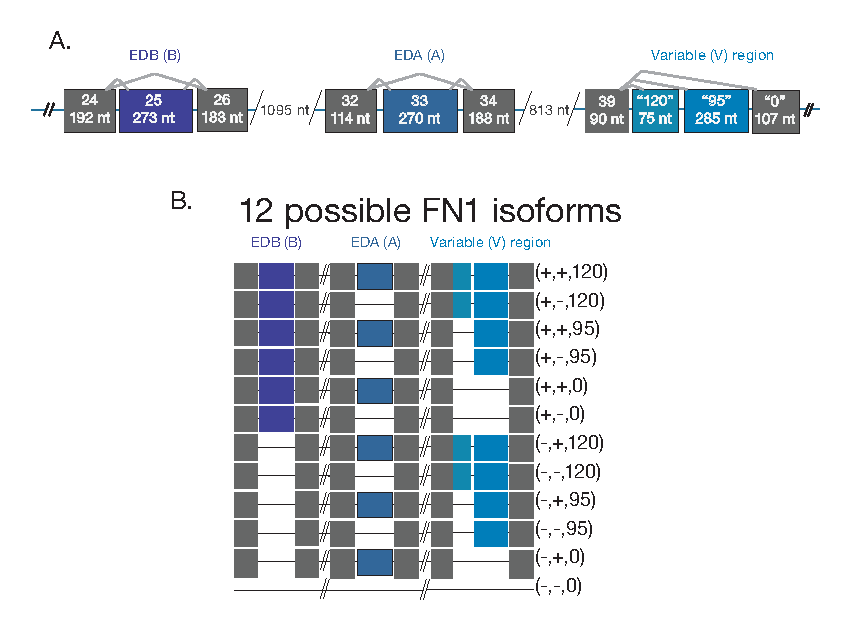
\includegraphics{Figures/Intro/Fibronectin.eps}
      \caption[Mouse \fn{} contains multiple sites of Alternative Splicing]
      {
        Mouse \fn{} contains multiple sites of Alternative Splicing\\[0.25cm]
        A) There are three highly-studied regions of alternative splicing in mouse \fn{}: Cassette exons EDB and EDA and the Variable(V)-region exon, which displays multiple 3\textprime~splice sites.  Each of these sites is separated by multiple constitutive exons. B) Considering simplistic splicing of these three exons, there are 12 different isoforms of mouse \fn{}.
        }
      \label{Intro:fig:mouseFn1}
      \end{figure}

    Some studies have investigated coordinated splicing between adjacent exons present in mRNA. The vertebrate genes \textit{4.1B} and \textit{4.1R} are members of the protein 4.1 family which encode cytoskeletal adaptor proteins. Both genes undergo splicing of a 5\textprime~first exon to distal second exons, skipping a stronger proximal 3\textprime~second exon \citep{Parra2008, Parra2012}. This is accomplished through ``intrasplicing'' involving an intronic sequence element (``intraexon'') only present when transcription begins at the upstream 5\textprime~exon. This allows the exon to ligate to the weaker distal 3\textprime~second exon via an intermediate splicing event.

    \textit{Cis}-acting sequences contained in intronic regions of a gene, a so-called Intronic Recognition Elements (IRE), has also been reported for the equine \textit{$\beta$-casin} gene. In this gene, an IRE bound to the exit channel of the elongating polymerase \citep{Lenasi2006}. IRE binding of the nascent RNA promotes inclusion of downstream cassette exons.

    Taking a more genome-wide approach \citet{Peng2008} examined human and mouse EST data looking for correlations between inclusion and exclusion of adjacent alternative splicing cassette exons. The authors note that positively correlated pairs of adjacent cassette exons typically resemble constitutive exons in similarity to the consensus splice sequences. Negatively and weakly correlated pairs are likely to be newly evolving exons whose sites have not evolved enough to be constitutively included.

    The most current and thorough study of intra-gene splicing coordination involves the \worms{} gene \slo{} \citep{Glauser2011, Johnson2011}. \slo{} is the \worms{} orthologue of the human BK channel gene \kcnma{}, which undergoes extensive alternative splicing \citep{Nilsen2010} via 13 cassette exons, potentially coding for over 1,000 different isoforms. \kcnma{} is developmentally, spatially, and tissue regulated and is involved in a diverse range of cellular processes, including hearing, circadian rhythms, urinary function, and vasoregulation \citep{Fodor2009a}.

    In worms, \slo{} can produce up to 12 different isoforms. \citet{Glauser2011} used TaqMan qPCR to demonstrate that individual alternative region inclusion frequencies do not correspond to complete isoform frequencies, suggesting an interdependent-splicing model. Interdependence was supported when mutations at one site altered both upstream and downstream sites of alternative splicing, separated by at least one other splicing event. After measuring the biophysical properties of the resulting protein isoforms \citep{Johnson2011} \citet{Glauser2011} conclude that coordinated alternative splicing is critical for proper BK channel function \textit{in vivo}. This study also identified an IRE that displayed some type of coordinated (or co-regulated effect) on alternative splicing.

    Indeed the Miller Spread was an early glimpse into another aspect of Nature's complexity. Described here are only a few examples of coordinated splicing. Genes like \fn{} and \slo{} have been carefully studied for decades. Yet each was done on a small, targeted scale. Increasing resolution of genome-wide data, better transcriptome assembly, and more rigorous analysis may reveal more examples of coordinated splicing decisions.

  \subsection{One Gene. Many Isoforms}
    \label{Intro:subsec:IsoformsPerGene}

    Researchers often uncouple evolutionarily intertwined processes such as transcription and splicing. A similar reductionist approach is to think of alternative splicing as a binary process: isoform A or B is produced by picking either exon A or B. What quickly becomes evident (to the detriment of researchers building transcriptome assembly algorithms) is that the combinatorial nature of alternative splicing makes it both a powerful means of generating isoform diversity \textit{and} a difficult problem to study \citep{Trapnell2012a}.

    \begin{figure} % alternative splicing Events per type barchart
      \centering 
      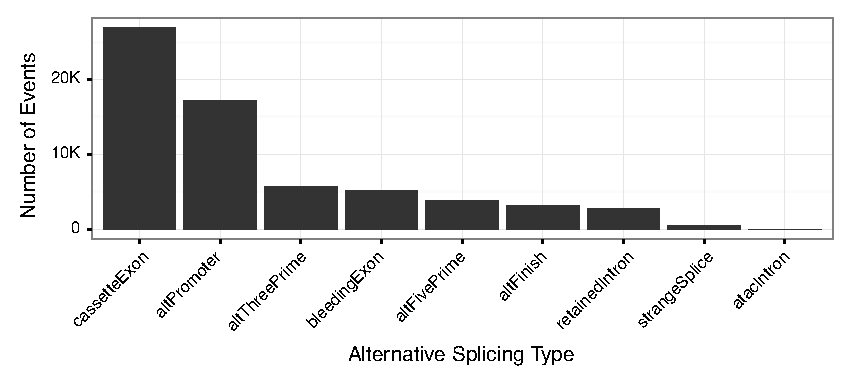
\includegraphics{Figures/Intro/ASEventTypesPlot.eps}
      \caption[Number of hg19 Alternative Event types]
      {
        Number of hg19 Alternative event types per gene\\[0.25cm]
        Alternative Event types per gene. ``cassetteExon'''s are complete exons that are either included or not. ``altPromoter'' indicates a different transcriptional start site, and thus typically a different first exon identity. ``alt[Five|Three]Prime'' refers to different use of 5\textprime~ and 3\textprime~ splice site use for a given exon. ``retainedIntron'' refers to including an intronic region of a gene in the final mRNA. ``atacIntron'' refers to an intron whose remove of which is performed via the minor spliceosome. ``strangeSplice'' according to UCSC is ``An intron with ends that are not GT/AG, GC/AG, or AT/AC. These are usually artifacts of some sort due to sequencing error or polymorphism.'' For complete list of definitions refer here: \url{http://genome.ucsc.edu/cgi-bin/hgTables} and refer to hg19:UCSC Genes:Alt Events schema. Accessed from RefSeq on 2014-03-24.
        }
      \label{Intro:fig:asEventsBarChart}
      \end{figure}

    A current attempt to investigate the breadth of combinations produced by alternative splicing is the ENCODE project \citep{Birney2007,Dunham2012}. The transcriptional annotation arm of the ENCODE project \citep{Djebali2012,Derrien2012} used data from 15 human cancerous cell lines and found genes produce \textasciitilde10 isoforms.

    The ENCODE project builds on prior evidence for the combinational quality of isoform expression \citep{Wang2008,Pan2008}. Most genes undergo multiple forms of alternative splicing (Figure \ref{Intro:fig:asEventsBarChart}). Despite the prevalence of complex alternative spliced genes, just a few genes are routinely used as examples to illustrate numerical possibilities and biological significance. For example, the human immune system relies heavily on alternative splicing for plastic antigen recognition and response \citep{Lynch2004}. Modulation of extracellular signaling proteins such as \textit{CD44} and cellular adhesion protein \textit{CD45} have been well-studied \citep{Zikherman2008,Ponta2003}.

    Alternative splicing in humans, however, does not seem to produce the extreme number of unique isoforms as alternative splicing of genes in some simpler animals, such as \flies{} (Figure \ref{Intro:fig:txPerFlyGene} and Table \ref{Intro:fig:txPerFlyGene}). Perhaps this reduced alternative splicing \textit{per gene} is due to gene specialization, with transcripts from different genes working in combination, as oppose to unique transcripts from \textit{same} gene \citep{Park2007}. For example, \flies{} have a single muscle myosin heavy chain gene (\textit{Mhc}) capable of producing up to 480 different isoforms through alternative splicing of 17 different cassette exons \citep{Bernstein1983a}. In contrast, mammalian genomes encode whole families of \textit{Mhc} genes that have duplicated, diversified, and specialized in function \citep{Weiss1996}. The use of gene families reduces the necessity for alternative splicing to generate molecular diversity. Section \ref{Intro:subsec:Dscam} discusses another example of \flies{} generating isoform diversity from a single gene, while the comparable human gene does not---the extracellular binding protein DSCAM.

    \begin{figure} % Number of transcripts per gene
      \centering 
      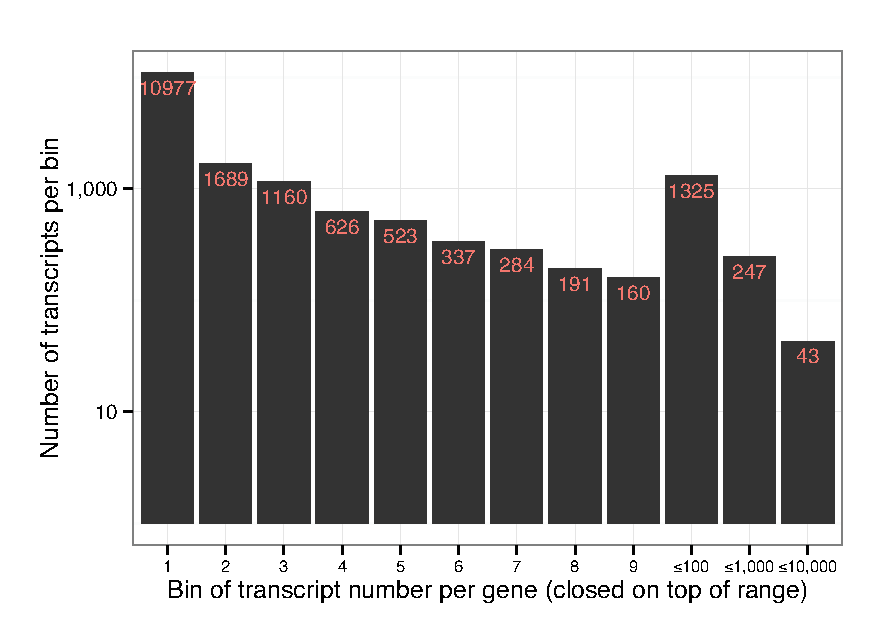
\includegraphics{Figures/Intro/NumberOFTranscriptsPerFlyGene.eps}
      \caption[Number of transcripts per \flies{} gene]
      {
        Number of transcripts per \flies{} gene\\[0.25cm]
        Data from \citep{Brown2014}, Supplemental Table 3. Number of transcript per bin, with bin sizes ``closed'' on the upper part of range.
        }
      \label{Intro:fig:txPerFlyGene}
      \end{figure}

    \begin{table} % Fly genes with 1000's of Tx
      \caption{Fly genes with >2,000 assembled transcripts according to \citep{Brown2014}.}
      \label{Intro:tab:FlyGenesWithManyTx}
      \renewcommand{\arraystretch}{0.5}
\small
\begin{tabular}[c]{l|r|r|r}
	\hline
	\textbf{Gene Name} & \textbf{\# Introns} & \textbf{\# Transcripts} & \textbf{\# Proteins}\\
	\hline
	Mhc & 60 &  2040 & 511\\
	\hline
	slo & 49 &  2070 & 279\\
	\hline
	ps & 30 &  2099 &  27\\
	\hline
	rg & 45 &  2178 &  23\\
	\hline
	shot & 60 &  2478 & 886\\
	\hline
	scrib & 53 &  2555 & 259\\
	\hline
	heph & 75 &  2876 &  52\\
	\hline
	CG42748 & 26 &  2876 &  51\\
	\hline
	rdgA & 35 &  3003 &  89\\
	\hline
	Mbs & 39 &  3080 & 119\\
	\hline
	CaMKI & 41 &  3992 &   7\\
	\hline
	par-1 & 48 &  4410 & 142\\
	\hline
	GluClalpha & 27 &  4945 & 188\\
	\hline
	Sap47 & 24 &  5011 &  49\\
	\hline
	Patronin & 50 &  5615 & 590\\
	\hline
	CG17838 & 37 &  8333 & 147\\
	\hline
	unc-13 & 52 &  8391 & 279\\
	\hline
	A2bp1 & 29 &  9055 &  58\\
	\hline
	Imp & 33 &  9131 &  12\\
	\hline
	pan & 38 &  9432 &  72\\
	\hline
	Sh & 40 & 15995 &  66\\
	\hline
	gish & 48 & 18972 & 142\\
	\hline
  \end{tabular}
      \end{table}

  \subsection{\flies{} \dscam{}}
    \label{Intro:subsec:Dscam}

    The gene most frequently used to demonstrate the combinatorial power of alternative splicing is \flies{} \dscam{}. The ``architecture'' of \dscam{} is rather unique, but as we see in Figure \ref{Intro:fig:txPerFlyGene} and Table \ref{Intro:tab:FlyGenesWithManyTx}, \flies{} contain numerous genes that generate tremendous isoform diversity \citep{Brown2014}. The basic structure of \dscam{} is shown in Figure \ref{Intro:fig:DscamArch}.

    Human \textit{Dscam} (Down Syndrome Cellular Adhesion Molecule) was identified while looking for genes on chromosome 21, specifically band 21q22, where extra copies are expressed in Down syndrome patients \citep{Yamakawa1998a}. \textit{Dscam} is a member of the immunoglobulin super family of proteins with extracellular adhesion functions. Human \textit{Dscam} undergoes some alternative splicing and is broadly expressed in the developing nervous system. Yet, it does not contain the same impressive number of cassette exons as \flies{} \dscam{}.

    \begin{figure} % Dscam Architecture
      \centering 
      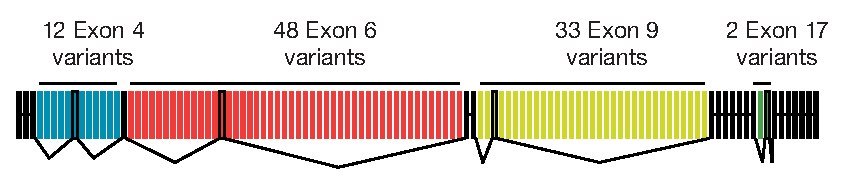
\includegraphics{Figures/Intro/DscamArch.eps}
      \caption[The architecture of the \flies{} gene \dscam{}]
      {
        The architecture of the \flies{} gene \dscam{}\\[0.25cm]
        \dscam{} has three \textit{clusters} or ``banks'' of alternative cassette exons that are included in a mutually-exclusive manner. The first bank, ``Exon 4'', contains 12 different variants, of which only one is ever included into the mRNA. Similarly, banks 6 \& 9 each contain 48 and 33 different variants, respectively. These three banks code for extracellular IgG domains, while the final region of alternative splicing, exon 17, encodes two different trans-membrane domains, again only one of which is included in the final mRNA.
          }
        \label{Intro:fig:DscamArch}
        \end{figure}

    Complex alternative splicing of \dscam{} was first noticed by the Zipursky lab in 2000 \citep{Schmucker2000}. While looking for proteins associated with \textit{dock} and \textit{pak}, two proteins important for neuronal growth cone guidance, they biochemically co-purified DSCAM1. Sequencing of \dscam{} clones revealed that all clones contained different combinations of exons 4,6, and 9. These three exons are chosen from three clusters of mutually-exclusive cassette exons, containing 12, 48, and 33 exons (Figure \ref{Intro:fig:DscamArch}). The initial report kicked off an exciting period of research into \dscam{} structure and function.

    Before the highlights of \dscam{} research are reviewed, it is illustrative to discuss some basic \flies{} anatomy. There are four anatomic regions where \dscam{} expression has been highly-studied:

    \begin{itemize} \itemsep0.5pt \parskip0pt \parsep0pt % Dscam expression regions
      \singlespacing
      \item Hemocyte cells of the immune system
      \item Larva Class IV da Neurons 
      \item Pupal Mushroom-body neurons in the developing brain
      \item Tetrad synapses of the eye
      \end{itemize}

    During larval development, \dscam{} is expressed in the da neurons of the larval body wall (Figure \ref{Intro:fig:DscamAnatomy}). The da neurons create a uniform sensory field that allow larva to respond to mechanical stimulus. Morphologically, da neurons resemble oak trees with broadly dispersed branches. In order to maximize coverage of the field, every \{cell::cell\} interaction (i.e. every synapse) must be a productive one. Molecularly, this is accomplished via an extracellular handshake between copies of DSCAM1. If this handshake feels too familiar, a stable, lasting, and \textit{productive} synapse is not encouraged \citep{Wojtowicz2004}. 

    The use of DSCAM1 to discern self from non-self is not unique to da neurons. It is also essential in the developing pupal brain. Here, \dscam{} is expressed in both axonal projections of neurons as they extend from Kenyon cell bodies and bifurcate into the two different mushroom body lobes \citep{Zhan2004}. 

    Finally, the involvement of \dscam{} in the innate immune system of insects has been demonstrated \citep{Watson2005,Dong2006}. DSCAM1 recognizes antigen via similar self vs non-self interactions.

    \begin{figure} % Dscam Anatomy
      \centering 
      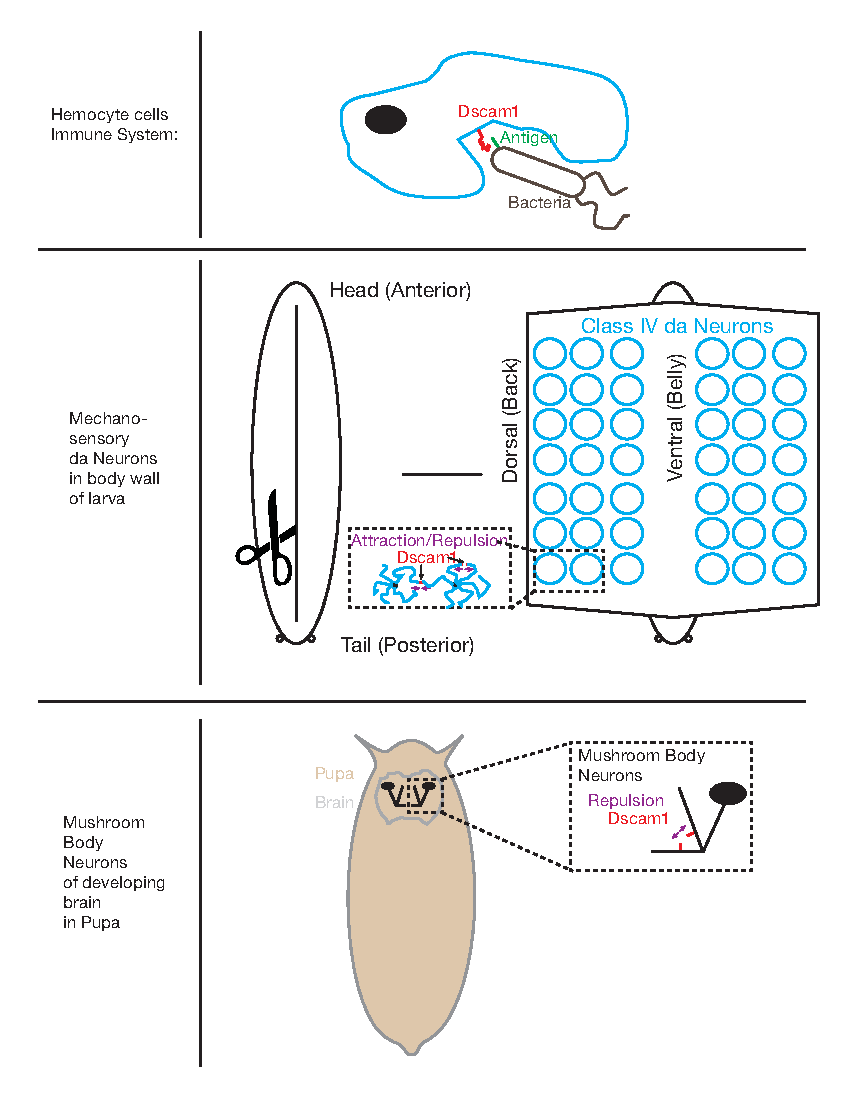
\includegraphics{Figures/Intro/DscamAnatomy.eps}
      \caption[Important sites of \dscam{} expression in \flies{}]
      {
        Important sites of \dscam{} expression in \flies{} \\[0.25cm]
        \dscam{} has been high-studied in four different regions/cell types. (1) Hemocytes of the immune system, where DSCAM1 is involved in antigen recognition; (2) In Class IV da neurons, which sense mechanical stimulation of the larval body wall; (3) In mushroom body neurons of the pupal developing brain; and (4) (not shown) in Tetrad neurons of the eyes.
        }
      \label{Intro:fig:DscamAnatomy}
      \end{figure}

    How diverse are \dscam{} isoforms? Are isoforms different between cells? How is diversity generated? Are isoforms different among tissues or in individual cells? These are the questions that research into \dscam{} has sought to answer over the last 14 years.

    Soon after the initial \dscam{} report \citet{Celotto2001} investigated \dscam{} developmental regulation. They focused on the 12 variants of cluster 4 and observed regulation of exon 4.2. Embryonic transcripts show little inclusion of this exon while adult transcripts show frequent inclusion. Exon 4.8 displayed the opposite behavior. Similar regulation of cluster 4 exons was also observed in a closely related species, \textit{Drosophila yakuba}.

    In 2004, \citet{Neves2004} used a specially designed microarray to robustly characterize \dscam{} molecular diversity. They observed inclusion of virtually all alternative exons from clusters 4, 6, and 9. Additionally, they examined \dscam{} transcripts obtained from single-cell originating colonies and reported that multiple \dscam{} transcripts were expressed per cell. They estimated that each cell, depending on type, contained between 7--50 different combinations. As discussed above, the use of microarrays to perform this analysis precluded observing any potential coordination between variant exons.

    Quickly after \citet{Neves2004} published their results, the Zipursky lab also published a microarray study of \dscam{} isoforms \citep{Zhan2004}. They focused their analysis on neurons of the developing mushroom body (Figure \ref{Intro:fig:DscamAnatomy}). Not only did they also show that most \dscam{} combinations are likely produced at some level, but that diversity of isoforms is required for bifurcation of neurons into different lobes of the developing mushroom body. These results highlighted a critical function for self vs non-self determination via DSCAM1-mediating extracellular interaction.

    How is mutually-exclusive exon usage among 48 different options possible? \citet{Graveley2005b} observed a single ``Docking site'' within the intronic sequence just 5\textprime~to exon 6.1. This docking site was conserved among 15 insect species examined, from closely-related \textit{Drosophila simulans} to a distantly-related \textit{Tribolium castaneum} (Red flour beetle). Astonishingly, the docking site was complementary to ``selector sites'' within intronic regions just 5\textprime~of each of the 48 variant exons. A model was proposed where \{docking::selector\} interaction is required to choose which variant exons is included, while a splicing regulator protein, likely an hnRNP due to the repressive nature of the interaction, binds to unused selector sites contained in the pre-mRNA \citep{Graveley2000}. Additional mechanisms have been reported for other clusters, including the \textit{iStem} \citep{Kreahling2005} in cluster 4, and the hnRNP protein hrp36 \citep{Olson2007}.

    \citep{Neves2004} examined \dscam{} expression in hemocyte cells, and their results clearly show reduced variability in cluster 9 inclusion. Virtually all of the signal obtained from hemocyte cells for cluster 9 was seen in variants 9.[6,9,13,30,and 31]. \citep{Watson2005} also examined \dscam{} expression in hemocyte cells, comparing it to that of neuronal cells. They propose that secreted forms of \dscam{} are essential for a robust innate immune system in insects, a finding that has also been observed in mosquitoes \citep{Dong2006}. Involvement of \dscam{} in the insect innate immune system highlights how nature has applied one gene that produces extreme molecular diversity to multiple problems involving determining self from non-self \citep{Hemani2012,Shi2012a, Hattori2008}.

    In 2007 the Zipersky lab published \citep{Hattori2007} the first in a series of genetic reports describing the function and diversity of \dscam{}. Using homologous recombination, \citet{Hattori2007} showed that \dscam{} diversity is required for proper neural wiring but that individual neuronal-isoform identity is not important. Two years later, \citet{Hattori2009} observed that flies capable of expressing at least 4,752 different \dscam{} isoforms were indistinguishable from wild-type controls. This series was recently advanced with another tour-de-force of genetic manipulation. \citet{Miura2013b} used a collection of \dscam{} mutants allowing for visualization via GFP of specific cluster 4.X variant expression in real time. They concluded that a single neuron expresses multiple \dscam{} isoforms over time, and \dscam{} is expressed via ``stochastic and probabilistic'' mechanisms.

    Research into \flies{} \dscam{} has provided major advancements to our understanding of multiple aspects of transcription, including: 1) exon definition; 2) alternative splicing of cassette exons; 3) neuronal and cellular recognition; and finally 4) allows comparisons between how points 1--3 are accomplished among model organisms. See sections \ref{SeqZipPaper:sec:Results} for more information concerning \dscam{}.

\section{Nucleic Acid Ligation}
  \label{Intro:sec:Nucleic Acid Ligation}

  Section \ref{Intro:sec:Nucleic Acid Sequencing} discusses implications of cheap DNA and RNA sequencing to biomedical research. This section discusses how the ability to \textit{join} pieces of nucleic acid has also advanced our understanding of biology. A particular focus is placed on an enzyme with relevance to Chapters \ref{SeqZipPaper} and \ref{SeqZipMethod}---T4 RNA Ligase 2.

  \subsection{RNA-templated DNA-DNA ligation}
    \label{Intro:subsec:Ligation}

    In the late 1960's and early 1970's, the Lehman and Richardson labs characterized two workhorse-enzymes of molecular biology. Robert Lehman and colleagues, working at Stanford Medical School, first described the activity of \textit{polynucleotide-joining enzyme} from \textit{Escherichia coli} (now known as \textit{E. coli} DNA Ligase) \citep{Olivera1967b}. Work on this enzyme paralleled that from the Richardson lab at Harvard Medical School, where they focused on \textit{polynucleotide ligase} from \textit{Escherichia coli} infected with T4 bacteriophage (now known as T4 DNA ligase) \citep{Weiss1967a}. It became clear that while these two enzyme's shared a common mechanism---later elucidated by \citet{Modrich1973a}---they had important differences. First, T4 DNA ligase required ATP as a cofactor, which \textit{E. coli} DNA Ligase did not (it was later discovered that DNA ligase required NAD as a cofactor). Second, only T4 DNA ligase could catalyze ligation of blunt-ended DNA \citep{Tabor1987a}.

    \begin{figure}% Ligation Mechanism
      \centering 
      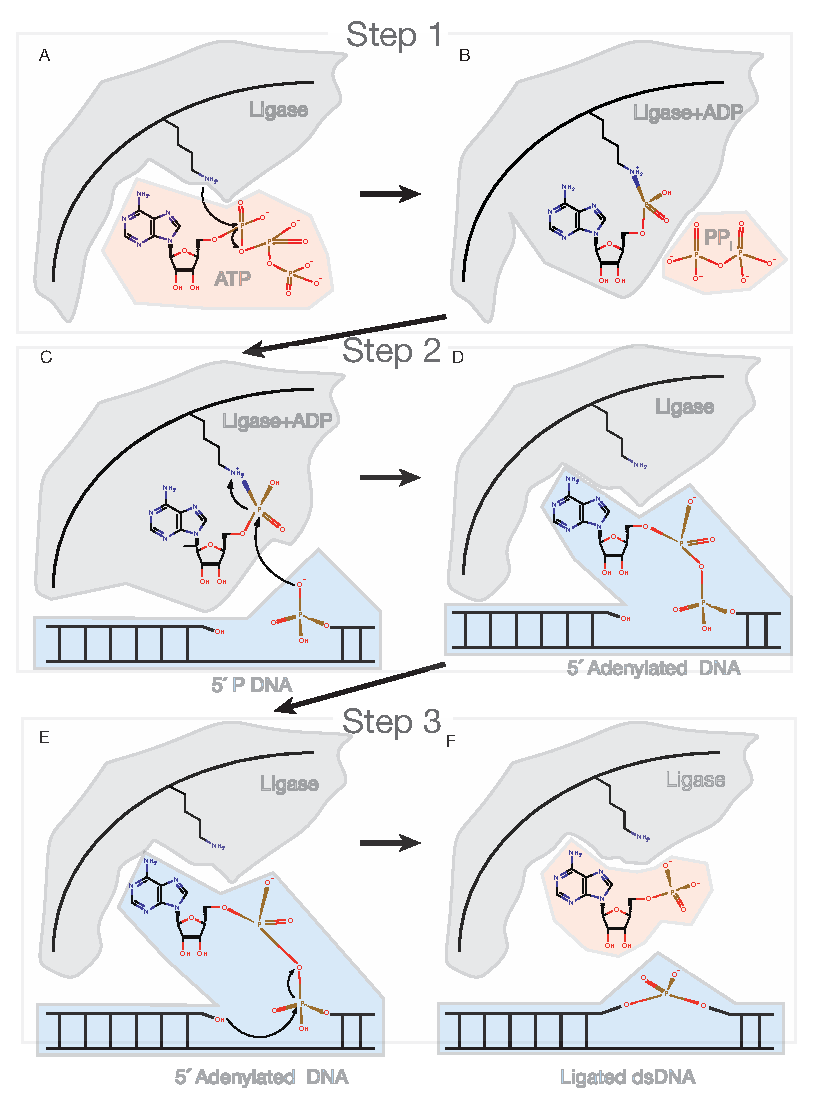
\includegraphics{Figures/Intro/LigationMechanism.eps}
      \caption[Mechanism of Rnl2 ATP-dependent ligation]
      {
        Mechanism of ATP-dependent ligation\\[0.25cm]
        Adapted from \citep{Nandakumar2006} and specifically for that of T4 RNA ligase 2.
        }
      \label{Intro:fig:Ligation Mechanism}
      \end{figure}

    The general mechanism of ligation (Figure \ref{Intro:fig:Ligation Mechanism}) involves three steps: Step 1 (A) the $\epsilon$-amino group from the active site lysine performs a nucleophilic attack on the $\alpha$-phosphate of ATP in solution. B) The ligase is now charged with AMP and inorganic phosphate (PPi) is freed into solution. C) Step 2: Nucleophilic attack by the 5\textprime~DNA phosphate on the 3\textprime~side of the nick to the AMP:ligase phosphate. D) Adenylated DNA is now competent for DNA ligation. E) Step 3: the 3\textprime~OH on the 5\textprime~side of the nick performs a nucleophilic attack on the 5\textprime~PO$_{4}$ across the nick, liberating AMP into solution. F) Sealed nick resulting in: Ligase, AMP, and dsDNA.

    In addition to elucidating the general mechanism of ligation, it was also discovered that T4 DNA ligase lacks a preference for terminal polynucleotide structures. The Khorana and Richardson labs both reported the activity of this enzyme on combinations of RNA and DNA duplexes \citep{Fareed1971, Kleppe1970b}. Both described an activity of T4 DNA ligase, RNA-templated DNA-DNA ligation, that is of particular relevance to this thesis work. Unlike T4 DNA ligase, \textit{E. coli} DNA Ligase, will not join DNA strands on an RNA template \citep{Bullard2006}. Soon after demonstrating these activities \textit{in vitro}, the Khorana lab reported detection of DNA generated \textit{in vivo} (i.e. by and organism) \citep{Besmer1972b}, setting up an orthogonal field (respective to PCR) of nucleic acid sequence characterization \citep{Conze2009c}.

    An enzyme that can catalyze an RNA-templated DNA-DNA ligation is a very useful molecular biology tool for two main reasons. First, using RNA as a ligation guide means no modification is made to the template. This contrasts cDNA analysis, where the RNA has been enzymatically converted by reverse transcription, potentially losing valuable RNA-coded information, such as modified bases. Second, synthesis of the DNA probes used in ligation is inherently easier and cheaper compared to synthesis of RNA probes (see section \ref{Disc:subsec:LNA-Containing ligamers and T39A Rnk2}). In addition to being cheaper, synthesis of DNA probes has become high-throughput since the adoption of microarrays as a standard gene expression measurement tool \citep{Schena1995a}. 

    A pair of papers from the Landegren lab first reported the utility of RNA-templated DNA-DNA ligation for analysis of RNA transcripts \citep{Nilsson2000,Nilsson2001}. The Fu lab applied this approach in a multiplex experimental design in collaboration with Illumina \citep{Li2012c,Yeakley2002}, while the Nilsson and Landegren labs developed a single molecule application \citep{Conze2010}. It is important to note that \textit{all} of these studies used T4 DNA ligase. Clearly, there is interest and utility in analyzing RNA in both high-throughput and multiplex experimental designs, using cheap DNA probes, and without cDNA conversion.
    % ER Comment:"It is still not clear how the used RNA-templated DNA-DNA ligation to analyse RNA without cDNA conversion. Maybe you could say a little bit more so that the reader does not have to read the papers to understand how they did it). "

    For more than 40 years after its first description, T4 DNA ligase was the only choice for RNA-templated DNA-DNA ligation. However, a recent publication from New England Biolabs (NEB) describes this activity by another well-studied ligase, Chlorella Virus PBCV-1 DNA ligase (herein Chlorella DNA ligase) \citep{Lohman2013c}. Chlorella DNA ligase is a long-studied enzyme and had been reported to \textit{not} display RNA-templated DNA:DNA ligation activity \citep{Ho1997b,Sriskanda1998c}. However, at high enough concentrations and under special buffer conditions (specifically a critical concentration of ATP), \citet{Lohman2013c} have shown that Chlorella DNA ligase will join two DNA strands hybridized to an RNA template. They further demonstrated that it performs no worse in this activity than traditional T4 DNA ligase \citep{Nilsson2001,Yeakley2002}.

    Building on the list of available enzymes that join hybrid polymer substrates Chapter \ref{SeqZipPaper} presents data supporting RNA-templated DNA-DNA ligation activity for another enzyme, T4 RNA Ligase 2.

  \subsection{T4 RNA Ligase 2}
    \label{Intro:subsec:Rnl2}

    Proteins of the T4 and T7 bacteriophages have been a boon for molecular biology. Without enzymes like polynucleotide kinase \citep{Richardson1965a}, T7 RNA polymerase \citep{Summers1970b}, and T4 DNA ligase \citep{Weiss1967a}, many essential manipulations of nucleic acids would have been impossible for decades. Obviously, these enzymes also have essential phage functions. T7 RNA polymerase is responsible for late stage replication of T7 phage transcripts, while T4 PNK works in concert with T4 DNA and RNA ligases to repair cleaved nucleic acids resulting from bacterial pathogen defense systems \citep{Wang2002b}. Specifically, T4 RNA ligase 1 (herein ``Rnl1'', also known as \textit{gene 63}) maintains phage replication by repairing tRNAs cleaved by an anticodon nuclease produced from the \textit{prr} locus \citep{Amitsur1987d}.

    Given the utility and importance of these enzymes, novel enzyme discovery is a fruitful area of research. The Shuman lab has a distinguished record of discovering and characterizing numerous such enzymes, including many involved in nucleic acid synthesis, modification, and repair. Through a BLAST search looking for novel ligases with sequences related to \textit{Trypanosoma brucei} RNA-editing ligases TbMP52 and TbMP48 \citep{Ho2002b}, they identified a gene in the T4 genome (\textit{gp24.1}) with motifs in correct arrangement, spacing, and number indicative of an RNA ligase.

    Initial biochemical purification and characterization of \textit{gp24.1} \citep{Ho2002b} revealed that it indeed codes for an RNA ligase, which was renamed T4 RNA ligase 2 (herein ``Rnl2''). Rnl2 is a 374 amino acid monomeric protein composed of 2 distinct domains initially purified as a 42-kDA His-tagged recombinant protein. The N-terminal domain (1--243) is responsible for steps (1) and (3) of the general ligation mechanisms (Figure \ref{Intro:fig:Ligation Mechanism}), while the C-terminal domain (244--329) is responsible for adenylation of the 5\textprime~PO$_{4}$ on the 5\textprime~residue at the 3\textprime~side of the nick, as shown in step (2). Rnl2 is routinely purified pre-adenylated and immediately poised for its first ligation. 

    In contrast to the N-terminal domain, which is composed of motifs typical to main ligases, the C-terminal domain is not contained in other DNA ligases. While the biological function of Rnl1 is known, the biological function of Rnl2 remains a mystery more than 12 years after its discovery \citep{Chauleau2013b}. However, there is some speculation that the flurry of research into bacterial CRISPR phage defense may reveal a role for Rnl2 \citep{Barrangou2007c,Chauleau2013b}.

    \begin{figure} % Rnl2 structure
      \centering 
      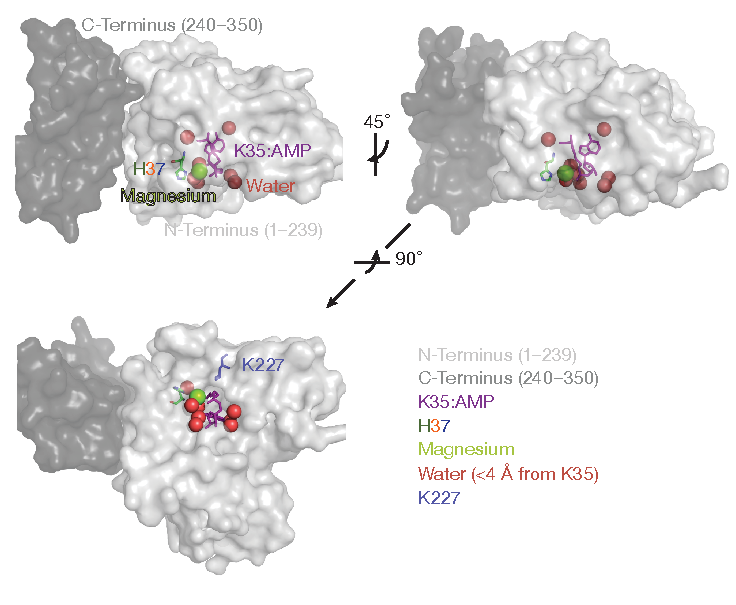
\includegraphics{Figures/Intro/Rnl2_Structure.eps}
      \caption[Structure and active site of pre-adenylated Rnl2]
      {
        Structure and active site of pre-adenylated of Rnl2\\[0.25cm]
        Rnl2 as crystalized and described by \citep{Nandakumar2006}. Structures from \{PDB:2HVQ\} were generated with PyMol. Top left) Rnl2 is composed of a C-terminal and N-terminal domain. Top Right) The active site of Rnl2 is highlighted. Bottom left) Active site of Rnl2 as shown from bottom. This face interacts with substrate.
        }
      \label{Intro:fig:Rnl2 General Structure}
      \end{figure}

    Mutational analysis crystal structure analysis of Rnl2 have identified key functional residues \citep{Ho2004, Nandakumar2006,Nandakumar2004a,Yin2003d}. The lysine residue at position 35 (K35) receives the AMP in Step 1. The K227 residue in the C-terminal domain is essential for both forward and reverse adenylation of the 5\textprime~PO$_4$ at the nick \citep{Viollet2011}. Mutation of H37 results in an \textasciitilde102 reduced ligation rate, indicating the important nature of this residue. Finally, T39 has been shown to interact with the 2\textprime~OH on the 3\textprime~side of the nick, preferring a C3\textprime~endo sugar pucker conformation (Figure \ref{Intro:fig:Rnl2 Active Site Residues}).

    Rnl2 has a minimal footprint of 13 nt, centered on the nick, and only requires magnesium for transfer of AMP to the 5\textprime~phosphate. Work done in the Shuman lab \citep{Nandakumar2006} observed that 2\textprime~deoxyribose residues on the 5\textprime~side of the nick (i.e. DNA) adopt an RNA-like sugar pucker, leading to the correct orientation of the 3\textprime~OH relative to the AMP leaving group and resulting in ligation. This conformation is of particular importance to results presented in Chapters \ref{SeqZipPaper} and \ref{SeqZipMethod}.

    \begin{figure} % Rnl2 Active site residues
      \centering 
      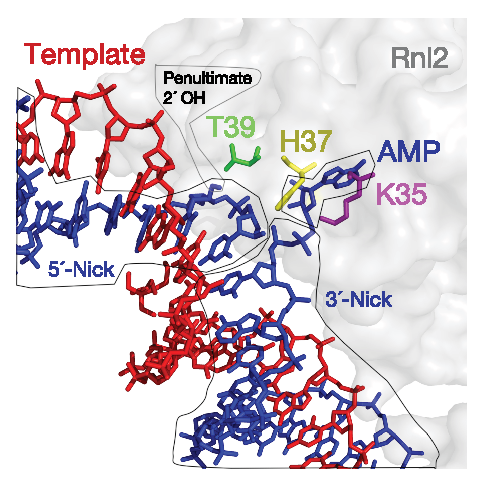
\includegraphics{Figures/Intro/Rnl2_Active_Site_Residues.eps}
      \caption[Active site of T4 RNA Ligase 2 with highlighted residues]
      {
        Active site of T4 RNA Ligase 2 with highlighted residues\\[0.25cm]
        Rnl2 complexed with nicked dsDNA as crystallized and described by \citep{Nandakumar2006}. Structures from \{PDB:2HVR\} and images generated with PyMol.
        }
      \label{Intro:fig:Rnl2 Active Site Residues}
      \end{figure}

    A modified version of Rnl2 containing only the N-terminal domain and a K227A point mutation (``Truncated mutant'') has no adenyltransferase activity \citep{Viollet2011}. In this case, adenyltransferase refers to the ligase transferring AMP from an adenylated substrate to itself; reverse chemistry of step 2 in Figure \ref{Intro:fig:Ligation Mechanism}). This mutant has been used in specialized cloning applications \citep{Ghildiyal2008, Hafner2008a, Viollet2011} that take advantage of this activity. In these reactions, the use of pre-adenylated 3\textprime~DNA adapters allows for selective ligation among already phosphorylated species by limiting the enzyme-catalyzed transfer of AMP from the adapter to other phosphorylated species. Use of this truncated mutant to create a hybrid RNA/DNA molecule has greatly improved high-throughput sequencing work-flows.

    Ligation of hybrid substrates (e.g.. DNA-templated RNA-DNA vs. DNA-templated DNA-DNA) have revealed general ligase substrate preferences. DNA ligases appear to prefer the residue bearing the 5\textprime~phosphate on the 3\textprime~side of the nick to be 2\textprime~deoxyribose, and have a relaxed requirement for the sugar on the 5\textprime~side of the nick. RNA ligases have the reverse preference, demonstrating higher activities when the 5\textprime~strand, 3\textprime~OH residue also bears a 2\textprime~OH. Rnl2 has an additional preference for an RNA residue at the penultimate 3\textprime~side of a residue \citep{Ho2002b,Ho2004, Nandakumar2004a, Nandakumar2006}. The two base requirement for RNA at the 5\textprime~side of the double stranded nick biases Rnl2 to join RNA:[RNA/DNA] strands. 

    Independent labs have measured that RNA-templated DNA-DNA joining activity of Rnl2 is below assay limits of detection \citep{Bullard2006}. However, results discussed Chapters \ref{SeqZipPaper} and \ref{SeqZipMethod} show that with enough enzyme and sensitive downstream measurements, Rnl2 will catalyze RNA-templated DNA-DNA ligation. Previous reports of Rnl2 lacking this activity are likely due to a single turnover mechanism in this reaction imposed by a non-typical sugar pucker of the ligated DNA trapping the enzyme on the duplex.

  \subsection{Ligases as molecular tools}

    Section \ref{Intro:subsec:Ligation} describes the identification and development of ligases as tools in molecular biology. Ligation of templated duplexes has multiple uses in cloning and sequence characterization. The following section (\ref{Intro:sec:Nucleic Acid Polymers}) discusses long nucleic acid polymers, specifically mammalian piRNA precursor transcripts. Little biology is known concerning these long transcripts. Chapters \ref{SeqZipPaper} and \ref{SeqZipMethod} discuss the application of Rnl2 to characterize long nucleic acid polymers.

\section{Nucleic Acid Polymers}
  \label{Intro:sec:Nucleic Acid Polymers}

  \citet{Fire1998} brought small RNAs to the forefront of research. Recently lncRNA research has been in similarly exciting period \citep{Khalil2009,Guttman2009}. Whether ``small'' or ``long'' all classes of RNA are polymers of ribonucleotides. This section will focus on an interesting class of nucleic acid polymer---mammalian piRNA precursor transcripts. These transcripts, which share similarities to traditional mRNAs, are processed into piRNAs. The section ends with a history of transcript assembly using HTS data.

  \subsection{It Started Small: Mammalian piRNAs}
  
    piRNAs are small RNAs that are 23--35 nt long. They are slightly longer than other small RNAs (e.g. miRNAs or siRNAs, which are 21 to 25 nt long). Contrary to other small RNAs, piRNA biogenesis does not require the double-stranded RNA-specific ribonuclease Dicer \citep{Vagin2006, Houwing2007} and it is believed they originate from single-stranded RNA precursor transcripts. Yet, similar to other small RNAs, they do bind a subgroup of the Argonaute family of proteins, PIWI proteins, from which their name is derived (\textit{PIWI Interacting RNAs}). 

    \citet{Aravin2001} first identified piRNAs in \flies{} originating from the \textit{Su(Ste)} locus as heterogeneous 25--27 RNAs essential for silencing of \textit{Stellate} and, more importantly, male fertility. In the few years since the initial report, piRNAs have been cataloged, characterized, manipulated and mutated, especially in \flies{} \citep{Siomi2011,Luteijn2013,Hirose2014}. The most famous function for piRNAs in \flies{} is suppression of transposon transcripts during gametogenesis \citep{Malone2009}. The Ping-Pong model elegantly explains how this might be accomplished: cyclic cleavage of transposon transcripts and piRNA precursor transcripts \citep{Brennecke2007,Gunawardane2007}. Yet, it appears that piRNAs have diversified beyond transposon silencing.

    Four reports in 2006 defined the beginning of mammalian piRNA research \citep{Aravin2006,Grivna2006,Girard2006,Lau2006}. Each observed small 23--35 nt RNA species that bound PIWI proteins. They also noticed that when aligned to the genome, most mapped to ``clusters'' of discrete genomic loci, similar to flies.

    Overtime, it became clear that mammalian piRNAs can divided into three major classes (Figure \ref{Intro:fig:Mammalian piRNA classes}). There are also three PIWI proteins in mice, each displaying a distinct expression profile during development and an association with piRNAs of a specific length.

    \begin{landscape}
      \begin{figure} % Mammalian piRNA classes
        \centering 
        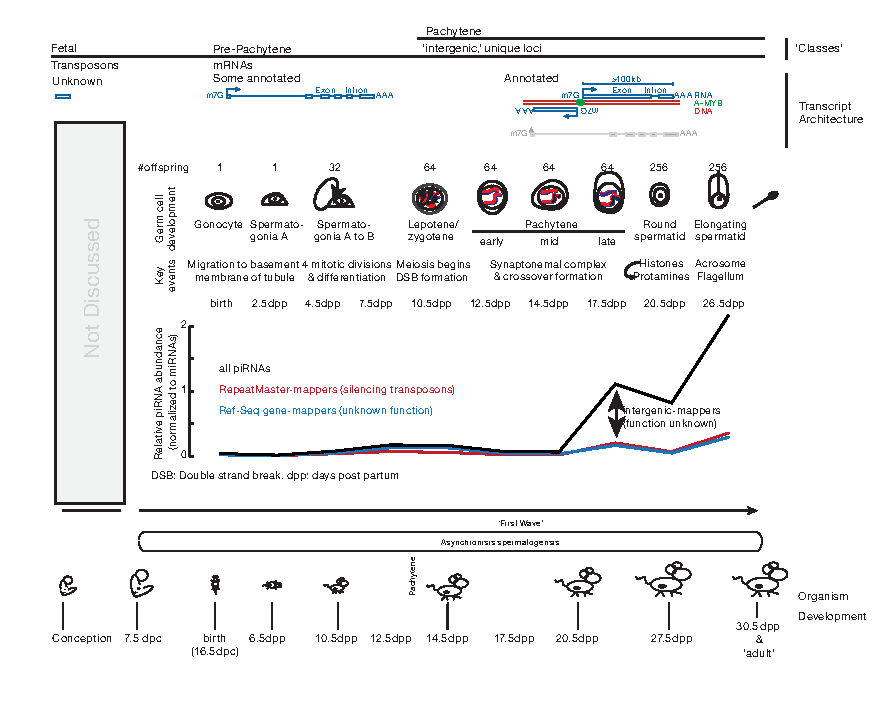
\includegraphics{Figures/Intro/MammalianPiRNAClassesOverTime.eps}
        \caption[Different Classes of mammalian piRNAs]
        {
          Overall view of the three classes of mammalian piRNAs. Figure design assisted by \href{mailto:xin.li@umassmed.edu}{Xin Zhiguo Li}.
          } \label{Intro:fig:Mammalian piRNA classes}
        \end{figure}
      \end{landscape}

    \textit{Fetal piRNAs} (or ``prenatal'') are present before birth. These piRNAs tend to be short, bind the PIWI protein MIWI2 (PIWIL4) in mice, and have sequences found in transposable elements \citep{Carmell2007}. Quickly following MIWI2 in expression is the PIWI protein MILI (PIWIL2). It is during the ``fetal'' stage of piRNA biogenesis in mice that, in order to silence expression of transposons during germ line formation, MIWI2 and MILI undergo ping-pong amplification, similar to that observed in flies \citep{Kuramochi-Miyagawa2004, Aravin2006, Aravin2008a,Aravin2008}. Importantly, this activity has not been observed in adult testes.

    During the first three weeks of a male mouse's life the process of spermatogensis is in its ``first wave'' and sperm cells are synchronized \citep{Oakberg1956b, Laiho2013a}. After the first wave and for the rest of the adult lifespan, sperm in the testes are not synchronized. Instead there is a continuum of sperm production. Therefore, it is during the first wave that specific stages of can be easily isolated and studied. The next two classes of piRNAs are named according to their expression respective to an important milestone in gametogensis---the pachytene stage of meiosis I when chromosomes pair up, cross over, and exchange genetic material. 

    \textit{Pre-pachytene piRNAs}, historically but confusingly grouped with fetal piRNAs, are expressed just before birth and continue to be expressed throughout the mouse lifespan. These piRNAs tend to map to traditional, annotated, protein-coding genes. During the ``neonatal stage'' pre-pachytene piRNAs are bound by the only PIWI protein expressed at that time, MILI. Also, piRNA expressed during the pre-pachytene stage shift from mostly transposon-mapping to protein coding gene 3\textprime~UTR mapping \citep{Robine2009}.

    The last class, \textit{pachytene piRNAs}, are extremely abundant compared to pre-pachytene piRNAs in adult testes \citep{Girard2006, Lau2006, Li2013h}. They bind another Piwi protein MIWI (PIWIL1). The genomic origin of pachytene piRNAs, often unique in terms of genomic sequence, often fall within ``gene deserts.'' Pachytene piRNA clusters are actually genes (aka: ``piRNA-producing loci'') encoding very long single-stranded transcripts devoid of introns (see section \ref{SeqZipMethod}) \citep{Li2013h}. This gene architecture makes the pachytene piRNA loci some of the most interesting RNA-producing regions of the mammalian genome. 

    Except for the uniquely-mapping quality of pachytene piRNA loci, their transcripts are comparable to piRNA clusters in flies, such as \textit{flamenco}. \textit{Flamenco} transcripts can be abolished by inserting a P-element into a putative promoter, as measured by northern blot looking for piRNAs generated 168 kb downstream (Figure \ref{Intro:fig:flamenco} \citep{Brennecke2007,Goriaux2014}. Similarly, transcription of pachytene piRNA loci requires \amyb{}, and piRNAs hundreds of thousands of nt downstream from annotated 5\textprime~ ends are not seen in \amyb{} mutant mice (see Chapter \ref{MolCel}).

    \begin{figure} % Flemenco Locus
      \centering 
      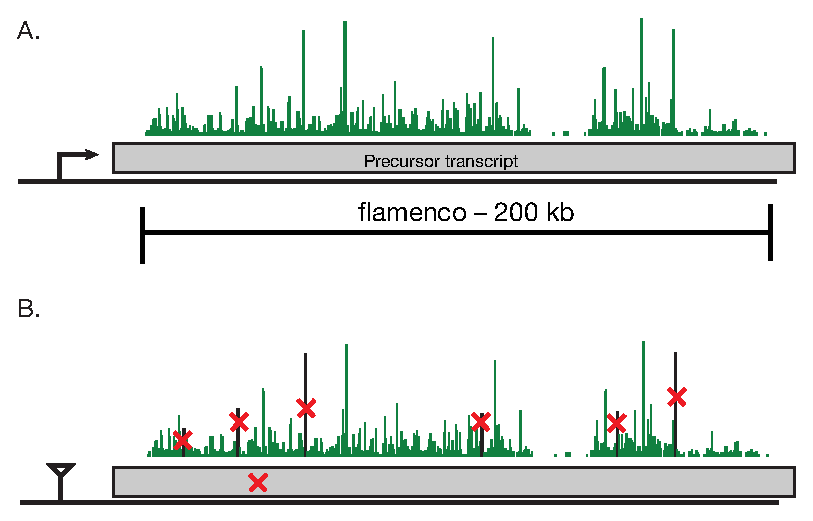
\includegraphics{Figures/Intro/FlamencoLocus.eps}
      \caption[Genetic evidence for long, continuous fly piRNA precursor transcripts]
      {
        A the \flies{} gene \textit{flamenco} is a graveyard for transposon sequences \citep{Pelisson1994}. Evidence for expression of a single-contiguous RNA transcript from \textit{flamenco} (A) is provided by a P-element insertion into the suspected promoter region (B). \citep{Brennecke2007} could not detect specific piRNAs (red X's) by northern blot in the P-element mutant.
        }
      \label{Intro:fig:flamenco}
      \end{figure}

  \subsection{From Long to Small: Precursor processing to mature piRNAs}
    \label{Intro:subsec:Processing of piRNAs in mice}

    The process by which a long, single-stranded piRNA precursor transcript become small mature piRNA is full of black boxes and question marks \citep{Li2013e}. Indeed, we are very unsure of many steps between transcription and terminal function of \{piRNA::PIWI\} complexes (PIWI-piRISC).

    For example, how do piRNA precursor transcripts exit the nucleus? This is not known in mice, but there are clues from \flies{}, where some piRNA clusters are bidirectionally transcribed and bound by the HP1 homologue Rhino \citep{Klattenhoff2009}. Rhino co-localizes with the DEAD box protein UAP56 near the perinuclear compartment known as nuage \citep{Zhang2012}. It is believed that Rhino and UAP56 assist in a hand off of large precursor transcripts across the nuclear envelope where they are bound by the nuage protein VASA \citep{Zhang2012}.

    Once precursor transcripts exit the nucleus they may enter chromatoid bodies (comparable to nuage in flies) \citep{Lim2007,Meikar2011,Zhang2012,Meikar2014} where they are proposed to be ``fragmented'' into shorter \textit{piRNA intermediates} \citep{Saito2010,Li2013}. However, the location of fragmentation is currently unknown in mice. In mice, the protein MitoPLD (aka: PLD6, or \textit{Zucchini} in \flies{}) is the proposed enzyme that catalyzes fragmentation, but this has only been studied in 10.5 dpp mice and therefore only for pre-pachytene piRNAs \citep{Watanabe2011a}.

    Slicing activity for \textit{Zucchini} has been observed \textit{in vitro} and is supported structurally \citep{Nishimasu2012,Ipsaro2012}. Its activity has yet to be shown \textit{in vivo} \citep{Luteijn2013}. Fragmentation may, or may not, impart the 5\textprime~U preference seen in mature piRNAs \citep{Gunawardane2007,Brennecke2007} and indeed Zucchini does not show a 5\textprime~U bias \textit{in vitro} \citep{Nishimasu2012,Ipsaro2012}. However, this preference may result from downstream sequence preference of PIWI-protein binding \citep{Cora2014}.

    Once fragmented into shorter RNAs, piRNA intermediates seem to be ``loaded,'' into a specific time- and expression-appropriate PIWI proteins (Figure \ref{Intro:fig:Mammalian piRNA classes}). Following ``loading,'' piRNA intermediates are trimmed down to the length characteristic of bound Piwi by the appropriately named, but \textit{hypothetical}, enzyme ``Trimmer'' \citep{Li2013}. Both ``Loading'' and ``Trimmer'' activity have not been shown in mammalian systems but are inferred from Silk worm (\textit{Bombyx mori}) cellular extracts of ovary-derived BmN4 cells \citep{Kawaoka2009}. Once trimmed, piRNAs are methylated on the 2\textprime~OH position by the enzyme HEN1 \citep{Horwich2007,Kirino2007,Ohara2007,Kawaoka2011}, but again this activity is not well-studied in mice. At this point, a mature piRNA, complexed with a PIWI protein (PIWI-piRISC), is poised to perform cellular function(s).

    \begin{figure}\small % Mammalian piRNA Pathway
     \centering 
     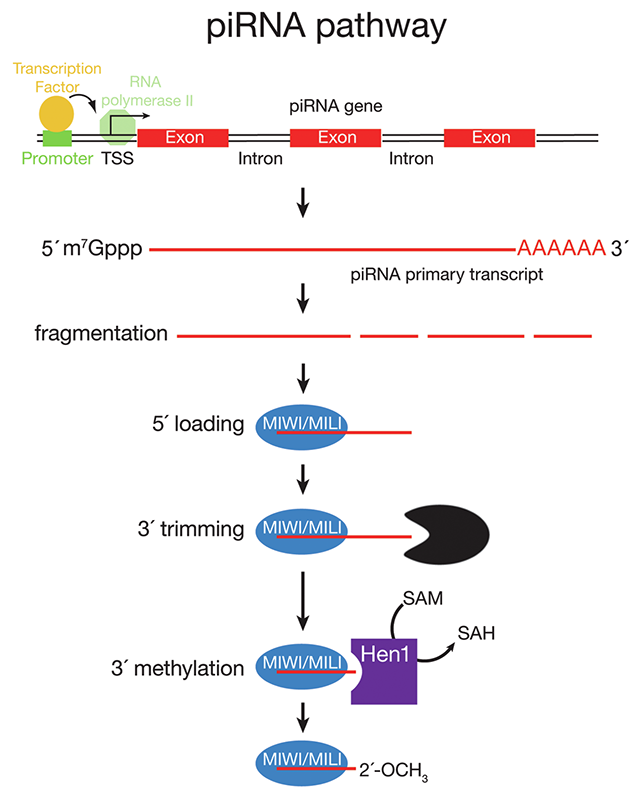
\includegraphics{Figures/Intro/mammalian_piRNA_pathway.png}
     \caption[A model for Mammalian piRNA biogenesis]
     {
       Figure taken from \citep{Li2013e}: A model for piRNA biogenesis. Primary piRNA transcripts are transcribed by RNA polymerase II and contain 5\textprime~caps, exons, introns, and poly(A) tails. The transcription of pachytene piRNA genes is controlled by A-MYB; transcription factor(s) (TF) controlling pre-pachytene piRNA genes remain to be discovered. Current models of piRNA biogenesis propose that PLD6 determines the 5\textprime~end of piRNA intermediates with lengths >30 nt. These intermediates are proposed to then be loaded into PIWI proteins. After PIWI binding, a nuclease is thought to trim the 3\textprime~end of the piRNA to the length characteristic of the particular bound PIWI protein. Finally, further trimming is prevented by addition of a 2\textprime~O-methyl group to the 3\textprime~end of the mature piRNA by the S--adenosylmethionine-dependent methyltransferase HEN1. Figure adapted from \citep{Li2013}.
       }
     \label{Intro:fig:Mammalian piRNA BioGensis}
     \end{figure}

    What are the cellular activities of PIWI-piRISC? MILI and MIWI2 have been shown to direct epigenetic LINE1 and IAP transposon silencing in the embryonic male germline \citep{Aravin2007,Carmell2007,Kuramochi2008}. Two studies \citep{DeFazio2011,Reuter2011} used point mutations in the catalytic triad of MIWI, MIWI2, and MILI to remove slicer activity. \citet{DeFazio2011} found that MIWI2-deficient mice are fertile, silence transposons, and display all signs of secondary piRNA biogenesis and concluded that MILI (which is sterile) was required for transposon silencing. This finding was later elaborated upon by \citet{DiGiacomo2013} to work in concert with other forms of epigenetic silencing to repress LINE1 expression. \citet{Reuter2011} focused on MIWI and found that it required for silencing of LINE1 transcripts long after they were epigenetically silenced (i.e. in the adolescent mouse).

    The above studies point to a familiar scenario of piRNA-mediated target cleavage and/or transcriptional silencing by PIWI-piRISC \citep{Meister2013}. Yet confusingly, HITS-CLIP of MIWI revealed that MIWI binds spermiogenic mRNAs without a piRNA guide \citep{Vourekas2012} and \citet{Reuter2011} demonstrated that slicing of target by MIWI RISC requires near perfect binding.

    How does does one reconcile these findings with the extremely uniquely-mapping quality of virtually all pachytene piRNAs? Put another way, if MIWI requires near perfect pairing between guide and target, and pachytene piRNAs perfectly pair with nothing else in the genome but antisense transcripts from their own loci, what is the mechanism of target recognition?

    Taken together, frustratingly little is known or internally consistent concerning biogenesis or function of mouse piRNAs. Indeed, even the catalytic nature of PIWI proteins is a debated topic \citep{Luteijn2013,Meister2013}. A recent report that the DNA modification 5hmC is high in piRNA intergenic gene bodies \citep{Gan2013}, combined with known functions of fetal PIWI-piRISC alludes to a function for self-mapping pachytene piRNAs.

    Perhaps the site of PIWI-piRISC function is not cytoplasmic. Fly PIWI is localized in the nucleus, and MILI and MIWI2 have been shown in induce DNA methylation \citep{Cox2000,Aravin2008}. This is a potentially misleading course of logic. Localization does not confirm interaction \citep{North2006} or function and inferring such from localization can be as dangerous as assuming cars function in parking lots. Finally, a extremely tantalizing additional potential function for mammalian piRNAs is that of genomic imprinting \citep{Watanabe2011}. This function is in good agreement with germ line-specific and developmentally timed nature of Piwi protein expression.

    In summary, there are many holes and black boxes in the story of mammalian piRNAs. Continued study is easily justified by the sterile phenotypes of all pathway mutants. Time will tell if mammalian piRNAs are involved in a satisfying process of biology or are crude side quest of Nature.

  \subsection{From Short to Long: Transcript Assembly}
    \label{Intro:subsec:Tx Assembly}

    Initial genome-wide HTS of piRNAs revealed a tremendous amount of biology \citep{Gunawardane2007,Brennecke2007}, but could provide little information as to the original transcriptional unit. The ability to reconstruct piRNA precursors had to wait for technological improvements in HTS read length and alignment algorithms.

    Working backwards from small RNA-Seq data to original transcription units was impossible. Mammalian piRNAs are too short (\textasciitilde30 nt) to allow for quality assembly using even the most current algorithms. They simply do not provide the sequence overlap necessary to build scaffolds. Also, repeat elements are extremely abundant in mice \citep{Nellaker2012}, and combined with short reads further reduce the ability to assemble full-length sequences. Therefore, it was necessary to sequence RNAs prior to mature piRNA formation.

    Even with longer read lengths and the best assembly algorithms, the 5\textprime~ and 3\textprime~ ends of long and diverse transcripts like piRNA precursors often requires a combination of multiple HTS datatypes \citep{Blower2013,Li2013e}. Tailored versions of RNA-Seq, such as CAP-Seq (see section \ref{Intro:subsec: History of HTS}), are not sufficient for accurate 5\textprime~end determination, and require orthogonal datasets to verify TSSs. Taking a page from lncRNA transcript discovery, complementary data sets such as ChIP-Seq of H3K4 methylated histones, a marker for transcriptional initiation can supplement RNA expression data \citep{Khalil2009}. More information about how multiple HTS datasets can be---and were used---to define the transcriptional unit of piRNA precursors transcripts is provided in Chapter \ref{MolCel}.

    General assembly of full length transcripts (not just piRNA precursor transcripts) is difficult for at least 3 reasons: (1) The transcriptome is expressed across 5 orders of magnitude and a typical RNA-Seq library contains many reads from a few highly-expressed genes and many fewer reads from lowly-expressed genes \citep{Blencowe2009}; (2) RNA-Seq libraries are often not created from a completely pure source of mRNA and can contain reads from other RNA classes (e.g. tRNAs) or intronic reads from pre-mRNAs; and (3) Reads are often much shorter than a typical mRNA, making it difficult to assign which read goes to which isoform of a given gene (see the ``connectivity problem'' discussed in section \ref{Intro:sec:Isoform Problem}. With these challenges in mind, what is the current state of transcript reconstruction (herein \textit{transcript assembly})?

    Computational transcriptome assembly of short reads is currently performed in one of two modes: genome-guided and genome-independent \citep{Garber2011a}. The difference between these two approaches is use of a high-quality genome during the assembly process. Popular assembly programs such as Cufflinks \citep{Trapnell2010} and Scripture \citep{Guttman2010} use genome-aligned short reads as the bases for calling transcripts. Genome-independent methods include Trinity, Oasis, and Velvet \citep{Haas2013c,Schulz2012,Zerbino2008}.

    As mentioned previously, constraints imposed by the dynamic range of RNA expression is the major complicating factor with current transcript assembly programs. These programs frequently generate short transcript fragments (``contigs'') due to poor coverage of long and lowly-expressed transcripts \citep{Rehrauer2013,Steijger2013}. Merging contigs into  continuous transcripts is a major goal. Improvements will surely come from greater sequencing depth, longer reads, and mRNA enrichment schemes, albeit with diminishing returns \citep{Chang2014c}. See section \ref{Disc:subsec:need for Tx assembly} for more thoughts concerning transcript assembly. Longer-term barriers include repetitive sequences, transcript secondary structure \citep{Wan2014}, and mRNA processing including hydrolysis and RT processivity \citep{Sharon2013}. Finally, multiple forms of mRNA enrichment and purification, specifically combining poly(A)+ tail and 5\textprime~CAP selection, can be used to increase the accuracy of mRNA transcript assembly \citep{Blower2013}. 

\section{Nucleic Acid 'Omics}
  \label{Intro:sec:Unique Time in Omics}

  Biomedical science has just taken a very sharp step (Figure \ref{Intro:fig:SeqCosts}) into an era of cheap genomics. Most questions, including those of gene expression, molecular interactions, and evolution no longer need be investigated on a small scale. Indeed formulating questions and hypothesis on a ``big scale'' should be considered from the very onset of a project. Combined broad and focused approaches will allow for maximal gains in knowledge. Yet much of the work required to reap maximal benefits from genome-wide approaches falls squarely on our own education and experience. See section \ref{Disc:sec:Final Thoughts} for concluding thoughts.

\cleardoublepage % Finish the chapter

  \chapter{SeqZip Publication} \label{SeqZipPaper} 
\lhead{Chapter 2. \emph{SeqZip Publication}} 
%----------------------------------------------------------------------------------------
\section{Abstract}\label{c1sec: Abstract}

\section{Introduction}\label{c2sec: Introduction}

	\begin{figure}[htbp] % Figure 1
		\centering 
		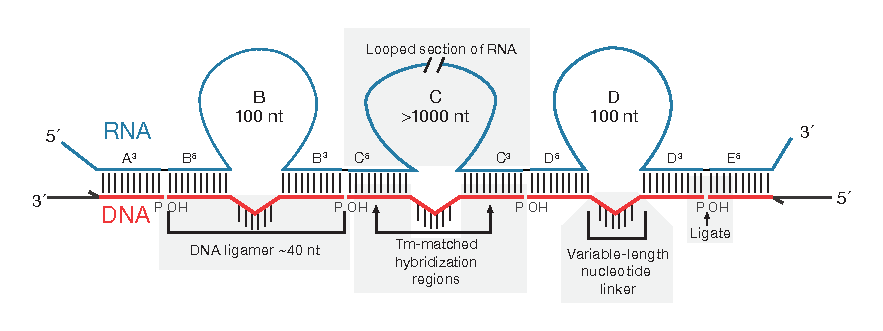
\includegraphics{Figures/SeqZipPaper/Roy2014Fig1.eps}
		\caption[SeqZip Diagram]
		{
			SeqZip Diagram\\
			\hl{Insert Figure Text}
			}
		\label{fig:Roy2014 F1}
		\end{figure}

\section{Results}\label{c2sec: Results}

	\subsection{Subsection 2}

		\begin{figure}[htbp] % Figure 2
			\centering 
			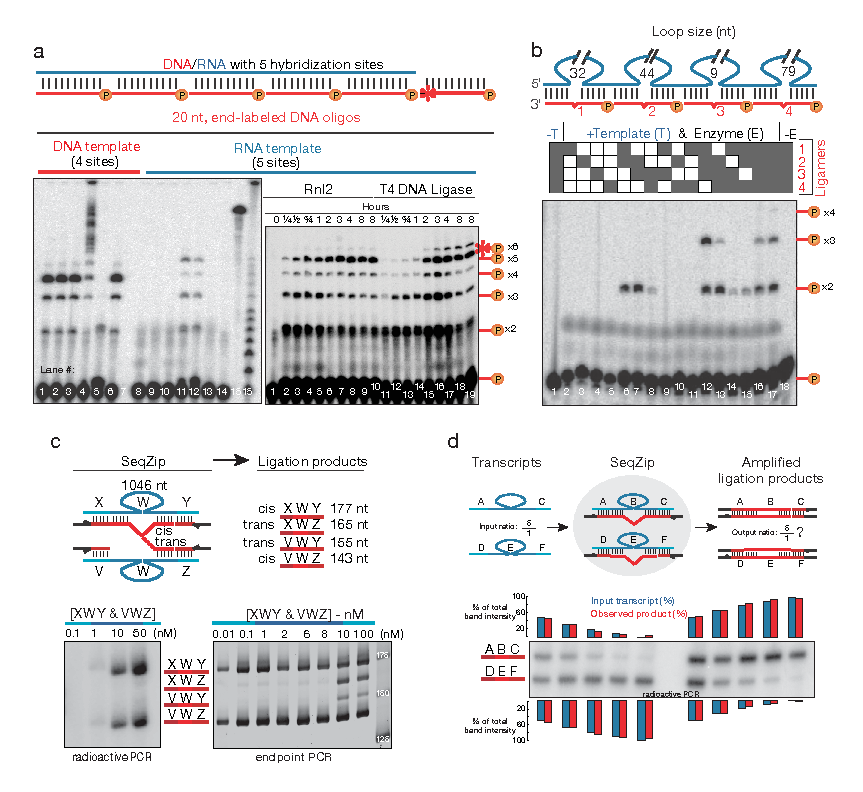
\includegraphics{Figures/SeqZipPaper/Roy2014Fig2.eps}
			\caption[SeqZip Diagram]
			{
				Roy et al Figure 2\\
				\hl{Insert Figure Text}
				}
			\label{fig:Roy2014 F2}
			\end{figure}

		\begin{figure}[htbp] % Figure 3
			\centering 
			\includegraphics{Figures/SeqZipPaper/Roy2014Fig3.eps}
			\caption[SeqZip Diagram]
			{
				Roy et al Figure 3\\
				\hl{Insert Figure Text}
				}
			\label{fig:Roy2014 F3}
			\end{figure}

		\begin{figure}[htbp] % Figure 4
			\centering 
			\includegraphics{Figures/SeqZipPaper/Roy2014Fig4.eps}
			\caption[SeqZip Diagram]
			{
				Rnl2 Panel\\
				\hl{Insert Figure Text}
				}
			\label{fig:Roy2014 F4}
			\end{figure}

		\begin{figure}[htbp] % Figure 5
			\centering 
			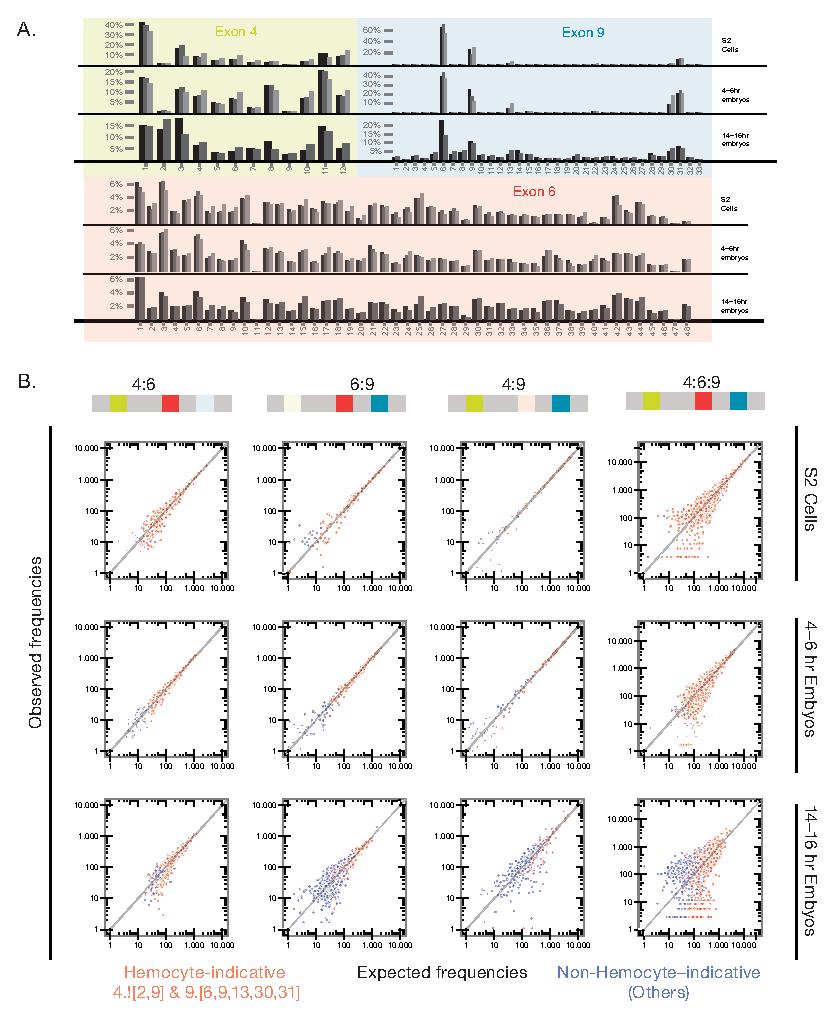
\includegraphics{Figures/SeqZipPaper/Roy2014Fig5.eps}
			\caption[SeqZip Diagram]
			{
				Roy et al Figure 5\\
				\hl{Insert Figure Text}
				}
			\label{fig:Roy2014 F5}
			\end{figure}

		\begin{figure}[htbp] % Figure 6
			\centering 
			\includegraphics{Figures/SeqZipPaper/Roy2014Fig6.eps}
			\caption[SeqZip Diagram]
			{
				Roy et al Figure 6\\
				\hl{Insert Figure Text}
				}
			\label{fig:Roy2014 F6}
			\end{figure}

		\begin{figure}[htbp] % Figure 7
			\centering 
			\includegraphics{Figures/SeqZipPaper/Roy2014Fig7.eps}
			\caption[SeqZip Diagram]
			{
				Roy et al Figure 7
				\hl{Insert Figure Text}
				}
			\label{fig:Roy2014 F7}
			\end{figure}]
			
\section{Discussion}\label{c2sec: Discussion}

\section{Methods}\label{c2sec: Methods}

\section{Supplemental Text}\label{c1sec: Supplemental Text}



  % !TEX root = /Users/royc/Google_Drive/Thesis/RoyC_Umass_Thesis.tex
\chapter{An Ancient Transcription Factor Initiates the Burst of piRNA Production during Early Meiosis in Mouse Testes} 
\label{MolCel} 
\lhead{Chapter 3. \emph{A-MYB Initiates Pachytene piRNA Production}}
%----------------------------------------------------------------------------------------
\section{Preface}
  \label{MolCel:sec:Preface}

  The contents of this have been published previously as:

  \begin{quote}
    \itshape 
    \singlespacing
    \bibentry{Li2013h}
    \end{quote}

  For information not contained in this chapter (mainly supplemental tables), please refer to the following locations: 

  NCBI: \url{http://www.ncbi.nlm.nih.gov/pubmed/23523368} \\
  Molecular Cell: \url{http://www.cell.com/molecular-cell/abstract/S1097-2765(13)00172-X}

  Supplemental tables can also be found on the Zamore Lab website: \url{http://www.sciencedirect.com/science/article/pii/S109727651300172X#appd003}

\section{Introduction}
  \label{MolCel:sec:Introduction}

  P-element induced wimpy testis (PIWI)-interacting RNAs (piRNAs) can be distinguished from other animal small silencing RNAs by their longer length (typically 23\textendash 35 nt), 2\textprime-O-methyl-modified 3\textprime~termini, and association with PIWI proteins, a distinct subgroup of Argonaute proteins, the small RNA-guided proteins responsible for RNA interference and related pathways \citep{Kumar1998,Farazi2008,Kim2009,Thomson2009,Cenik2011,Aravin2008}. piRNA production does not require Dicer, the double-stranded RNA endonuclease that makes microRNAs (miRNAs) and small interfering RNAs (siRNAs), and piRNAs are thought to derive from single-stranded rather than double-stranded RNA \citep{Vagin2006, Houwing2007}.

  In most bilateral animals, germline piRNAs protect the genome from transposon activation, but also have other functions \citep{Aravin2001, Aravin2007a, Aravin2008a, Vagin2004, Brennecke2007, Carmell2007, Hartig2007, Kuramochi-Miyagawa2008, Ashe2012, Lee2012, Shirayama2012}. A few days after birth, the majority of piRNAs in the mouse testis are pre-pachytene piRNAs; 25\% of these piRNA species map to more than one location in the genome. A second class of piRNAs, typically derived from intergenic regions, has been reported to emerge in the mouse testis 14.5 days postpartum (dpp), when the developing spermatocytes synchronously enter the pachytene phase of meiotic prophase I. These pachytene piRNAs compose >95\% of piRNAs in the adult mouse testis. Loss of genes required to make pachytene piRNAs blocks production of mature sperm \citep{Deng2002c, Aravin2001, Reuter2011, Vourekas2012}. What triggers the accumulation of pachytene piRNAs when spermatocytes enter the pachynema is unknown.

  In Caenorhabditis elegans, each piRNA is processed from its own short RNA polymerase II (Pol II) transcript \citep{Gu2012}. In contrast, insect and mouse piRNAs are thought to be processed from long RNAs transcribed from large piRNA loci. Supporting this view, a transposon inserted into the 5\textprime~end of the flamenco piRNA cluster in flies reduces the production of flamenco piRNAs 168 kbp 3\textprime~to the insertion, suggesting that it disrupts transcription of the entire locus \citep{Brennecke2007}. High-throughput sequencing and chromatin immunoprecipitation (ChIP) has been used to define the genomic structure of the piRNA-producing genes of immortalized, cultured silk moth BmN4 cells \citep{Kawaoka2012}. However, for flies and mice, we do not know the structure of piRNA-producing genes, their transcripts, or the nature of the promoters that control their expression.

  Instead, piRNA loci have been defined as clusters: regions of the genome with a high density of mapping piRNA sequences \citep{Aravin2006,Girard2006, Grivna2006,Lau2006,Brennecke2007,Ro2007}. In reality, piRNA-producing loci correspond to discrete transcription units that include both intergenic loci believed to encode no protein \citep{Brennecke2007,Brennecke2008, Vourekas2012} and protein-coding genes that also produce piRNAs \citep{Aravin2007, Robine2009, Saito2009}.

  We used high-throughput sequencing data to define the genes and transcripts that produce piRNAs in the juvenile and adult mouse testis. Using these data, we identified the factor that initiates transcription of pachytene piRNA genes: A-MYB (MYBL1), a spermatocyte protein that serves as a master regulator of genes encoding proteins required for cell-cycle progression through the pachytene stage of meiosis \citep{Trauth1994, Bolcun-Filas2011}. A-MYB also initiates transcription of the genes encoding many piRNA biogenesis factors. The combined action of A-MYB at the promoters of genes producing pachytene piRNA precursor transcripts and genes encoding piRNA biogenesis proteins creates a coherent feedforward loop that triggers a >6,000-fold increase in pachytene piRNA abundance during the \textasciitilde5 days between the early and late phases of the pachytene stage of male meiosis. A-MYB also promotes its own transcription through a positive feedback loop. The A-MYB-regulated feedforward loop is evolutionarily conserved: A-MYB is bound to the promoters of both piRNA clusters and PIWIL1, TDRD1, and TDRD3 in the rooster (Gallus gallus) testis.

\section{Results}

  \subsection{Defining piRNA-Producing Transcripts in the Mouse Testis}
    \label{MolCel:subsec:Defining piRNA transcripts}

    To define the structure of piRNA-producing loci in the testis of wild-type adult mice, we assembled the transcripts detected by three biological replicates of strand-specific, paired-end, rRNA-depleted, total RNA sequencing (RNA-seq; Figure \ref{MolCel:fig:MolCelF1}A). We mapped reads to the mouse genome using TopHat \citep{Trapnell2009} and performed de novo transcriptome assembly using Trinity \citep{Grabherr2011} to identify unannotated exon-exon junctions. We used all mapped reads, including reads corresponding to unannotated exon-exon junctions, to perform reference-based transcript assembly (Cufflinks; \citep{Trapnell2010}.

    \begin{figure} % Figure 1
      \centering 
      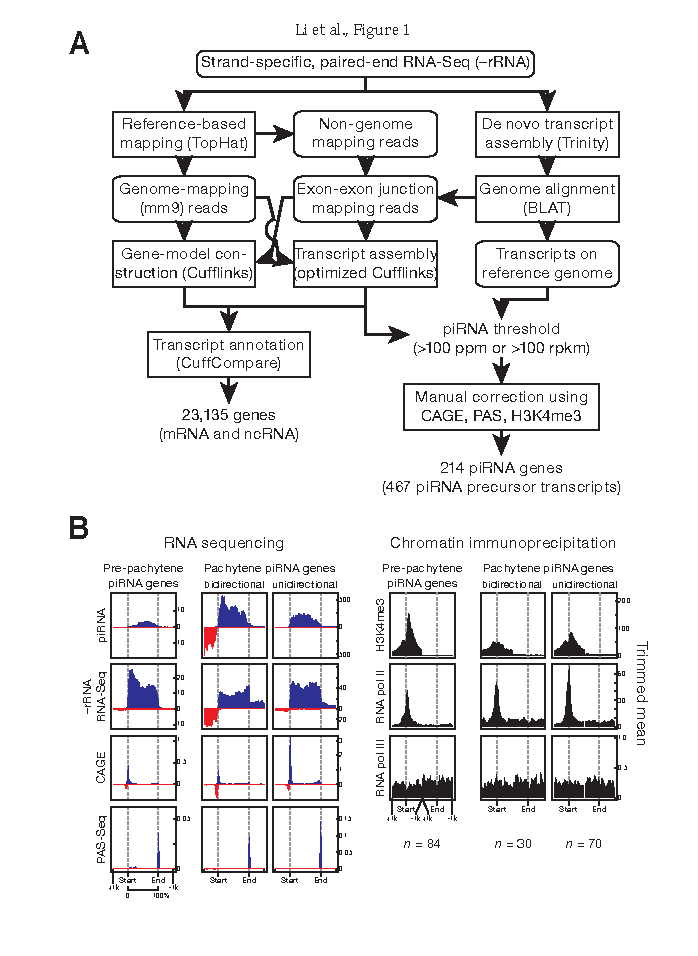
\includegraphics{Figures/MolCel/MolCel2013_Fig1.eps}
      \caption[piRNA Precursors are RNA Pol II Transcripts]
      {
        piRNA Precursors are RNA Pol II Transcripts\\[0.25cm]
        (A) Strategy to assemble the mouse testis transcriptome. Rectangles with rounded corners, input or output data; rectangles, processes. Decisions are shown without boxing.(B) Aggregated data for piRNA-producing transcripts (5\% trimmed mean). Oxidized small RNA (>23 nt) sequencing data were used to detect piRNAs; transcript abundance was measured using total RNA depleted of rRNA (RNA-seq). RNA Pol III data were from SRA001030. Dotted lines show the transcriptional start site (Start) and site of polyadenylation (End). See also Figure \ref{MolCel:fig:MolCelS1}.
        }
      \label{MolCel:fig:MolCelF1}
      \end{figure}
    \begin{figure} % Figure S1
      \centering 
      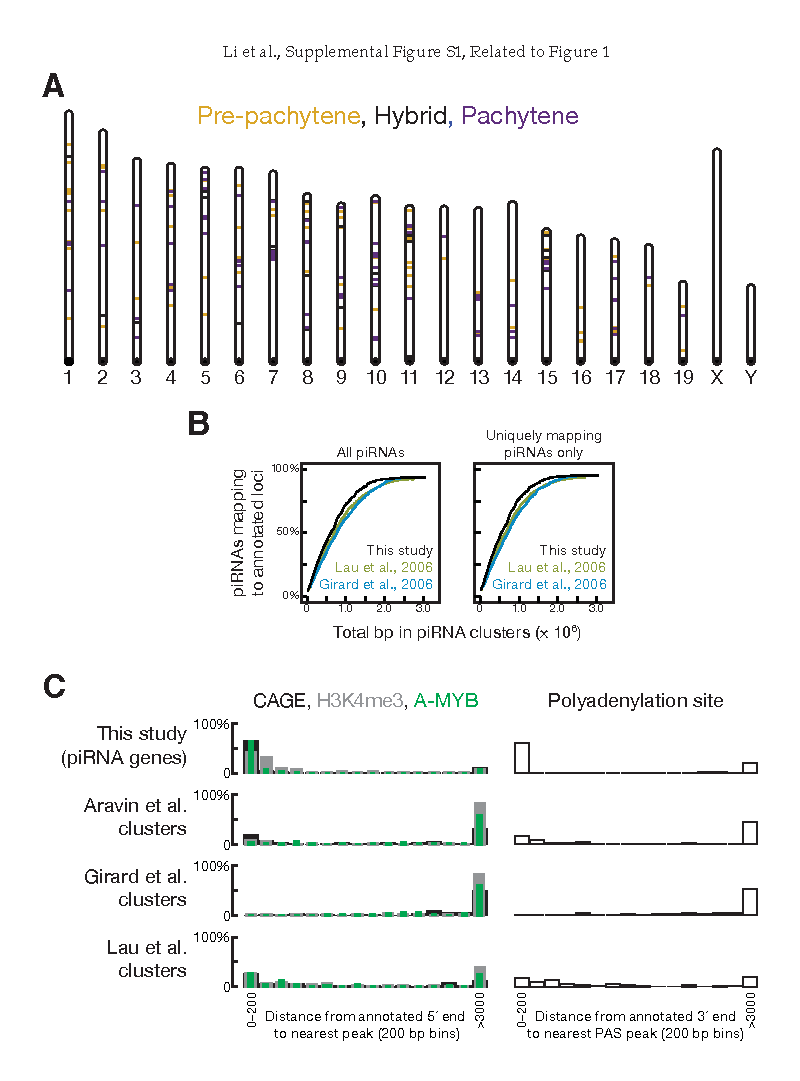
\includegraphics{Figures/MolCel/MolCel2013_FigS1.eps}
      \caption[The Major piRNA-Producing Genes of the Post-Partum Mouse Testis]
      {
        See subsection \ref{MolCel:subsubsec:cap:Figure S1} for full figure caption.
        }
      \label{MolCel:fig:MolCelS1}
      \end{figure}

    To identify the transcripts that produce piRNAs, we sequenced piRNAs from six developmental stages of mouse testes (10.5 dpp, 12.5 dpp, 14.5 dpp, 17.5 dpp, 20.5 dpp, and adult) and mapped them to the assembled transcripts. The first round of spermatogenesis proceeds synchronously among the tubules of the testis: mouse testes at 10.5 dpp advance no further than the zygotene stage (staging according to \citep{NEBEL1961}; 12.5 dpp to the early pachytene; 14.5 dpp to the middle pachytene; 17.5 to the late pachytene; and 20.5 dpp to the round spermatid stage. For each stage, we prepared two sequencing libraries: one comprising all small RNAs and one in which oxidation was used to enrich for piRNAs by virtue of their 2\textprime-O-methyl-modified 3\textprime~termini \citep{Ghildiyal2008}.

    To qualify as a piRNA-producing transcript, an assembled RNA was required to produce either a sufficiently high piRNA abundance (>100 ppm; parts per million uniquely mapped reads) or density (>100 rpkm; reads per kilobase of transcript per million uniquely mapped reads). These criteria retained both long transcripts producing an abundance of piRNAs and short transcripts generating many piRNAs per unit of length. To refine the termini of each piRNA-producing transcript, we supplemented the RNA-seq data with high-throughput sequencing of the 5\textprime~ends of RNAs bearing an N(5\textprime~)ppp(5\textprime~)N cap structure (cap analysis of gene expression; CAGE) and the 3\textprime~ends of transcripts preceding the poly(A) tail (polyadenylation site sequencing; PAS-seq). The assembled piRNA-producing transcripts likely correspond to continuous RNAs in vivo because the CAGE library used to annotate transcript 5\textprime~ends was constructed after two rounds of poly(A) selection. Thus, the RNA molecules in the library derive from complete transcripts extending from the 5\textprime~cap to the poly(A) tail (Figure \ref{MolCel:fig:MolCelF1}B). Conventional 5\textprime~and 3\textprime~RACE (rapid amplification of cDNA ends) analysis of piRNA-producing transcripts confirmed the ends of 16 loci (data not shown). To provide additional confirmation of the 5\textprime~end of each piRNA-producing transcript, we also determined the locations of histone H3 bearing trimethylated lysine 4 (H3K4me3), a histone modification associated with RNA Pol II transcription start sites \cite{Guenther2007}.

    \subsubsection{Caption for Figure \ref{MolCel:fig:MolCelS1}}
      \label{MolCel:subsubsec:cap:Figure S1}
      (A) Positions of the 214 major piRNA-producing genes on the 19 autosomes of mice. We detected no loci on the X or Y chromosomes. (B) Cumulative distributions for all piRNAs and for uniquely mapping piRNAs comparing the piRNA loci defined by our methods and by previous approaches \citep{Girard2006, Lau2006}. (C) Histogram of distances (in 200 bp bins) from the annotated 5\textprime~or 3\textprime~end of a piRNA gene (this study) or cluster to the nearest peak of reads from high-throughput sequencing for transcript 5\textprime~(CAGE-seq) or 3\textprime~(PAS-seq) ends, transcription start sites (H3K4me3) or A-MYB binding.

  \subsection{piRNA Precursor RNAs are Canonical RNA Pol II Transcripts}
    \label{MolCel:subsec:Precursors are Pol II Txs}

    The presence of 5\textprime~caps and poly(A) tails and the binding of histone H3K4me3 to the genomic DNA immediately upstream of the transcription start site of each piRNA locus suggest that piRNA transcripts are produced by RNA pol II \ref{MolCel:fig:MolCelF1}. Moreover, using antibodies to RNA pol II but not RNA pol III, ChIP-seq showed a peak at the transcription start site as well as polymerase occupancy across the entire piRNA gene (Figure \ref{MolCel:fig:MolCelF1}B; \citep{Kutter2011}. We conclude that piRNA transcripts are conventional RNA pol II transcripts bearing 5\textprime~caps and 3\textprime~poly(A) tails.

  \subsection{A Transcript-based Set of piRNA Loci}
    \label{MolCel:subsec:A TX-based set of piRNA loci}

    Our transcriptome assembly yielded 467 piRNA-producing transcripts that define 214 genomic loci (Figure \ref{MolCel:fig:MolCelS1}A and Table S1). Among the \textasciitilde2.2 million distinct piRNA species and \textasciitilde8.8 million piRNA reads from the adult mouse testis, the 214 genomic loci account for 95\% of all piRNAs.

    Previous studies defined piRNA clusters based solely on small RNA sequencing data \citep{Girard2006, Lau2006, Aravin2007a}. Our approach differs in that it (1) uses RNA-seq data, whose greater read length facilitates the identification of introns, allowing us to define the architecture of piRNA precursor transcripts and (2) uses CAGE, PAS-seq, and H3K4me3 ChIP-seq data to refine the 5\textprime~and 3\textprime~ends of the piRNA transcripts. Consequently, the piRNA loci presented here account for more piRNAs using fewer genomic base pairs than those previously defined (Figures \ref{MolCel:fig:MolCelS1}B and \ref{MolCel:fig:MolCelS1}C; \citep{Lau2006, Girard2006}. Our piRNA-producing loci include 41 piRNA loci that escaped previous detection \citep{Girard2006, Lau2006, Aravin2007a}, 37 of which contain introns. The 41 loci account for 2\% of piRNAs at 10.5 dpp and 0.36\% in the adult testis.

  \subsection{Three Classes of piRNAs During Post-Natal Spermatogenesis}
    \label{MolCel:subsec:Three Classes of piRNAs in testes}

    Mice produce three PIWI proteins: MIWI2 (PIWIL4), which binds piRNAs in perinatal testis \citep{Carmell2007, Aravin2008a}; MILI (PIWIL2), which binds piRNAs at least until the round spermatid stage of spermatogenesis \citep{Kuramochi-Miyagawa2004, Aravin2006, Aravin2007a}; and MIWI (PIWILl), which is first produced during the pachytene stage of meiosis \citep{Deng2002c}. From 10.5 to 20.5 dpp, piRNA abundance increases and longer piRNAs appear, reflecting a switch from MILI-bound piRNAs, which have a 26-27 nt modal length \citep{Montgomery1998, Aravin2006, Aravin2008a, Robine2009}, to MIWI-bound piRNAs, which have a 30 nt modal length (Figure \ref{MolCel:fig:MolCelS2}A; \citep{Reuter2009, Robine2009}. This switch occurs at the pachytene phase of meiosis. MILI-bound pre-pachytene piRNAs predominate before the onset of pachynema; at the pachytene and round spermatid stages, most piRNAs are MIWI-bound pachytene piRNAs.

    We used hierarchical clustering to analyze the change in piRNA abundance from 10.5 to 20.5 dpp for the 214 genes defined by our data (Figures \ref{MolCel:fig:MolCelF2}A and \ref{MolCel:fig:MolCelS2}A and Table S2). Three types of piRNA-producing genes were identified according to when their piRNAs first accumulate and how their expression changes during spermatogenesis: 84 pre-pachytene, 100 pachytene, and 30 hybrid loci. At 10.5 dpp, the earliest time we evaluated, 84 genes dominate piRNA production (median piRNA abundance per gene = 16 rpkm; Figure \ref{MolCel:fig:MolCelF2}B). Nearly all (81 out of 84) were congruent with protein-coding genes. The 84 pre-pachytene piRNA genes account for 13\% of piRNAs at 10.5 dpp, but only 0.31\% of piRNAs in the adult testis. Of the pre-pachytene piRNAs accounted for by the 84 loci, 15\% derive from 31 piRNA-producing genes that, to our knowledge, have not previously been described.

    \begin{figure} % Figure 2
      \centering 
      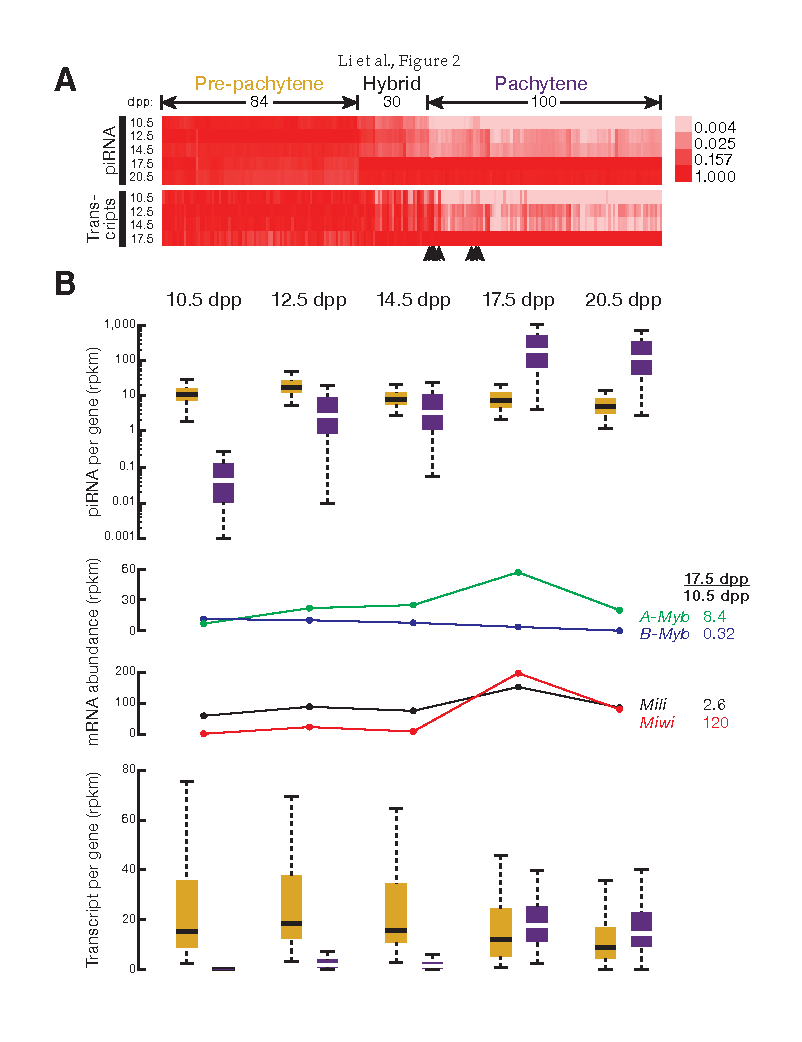
\includegraphics{Figures/MolCel/MolCel2013_Fig2.eps}
      \caption[Three Classes of piRNA-Generating Loci]
      {
        See subsection \ref{MolCel:subsubsection:cap:Figure F2} for full figure caption.
        }
      \label{MolCel:fig:MolCelF2}
      \end{figure}
    \begin{figure}\tiny % Figure S2
      \centering 
      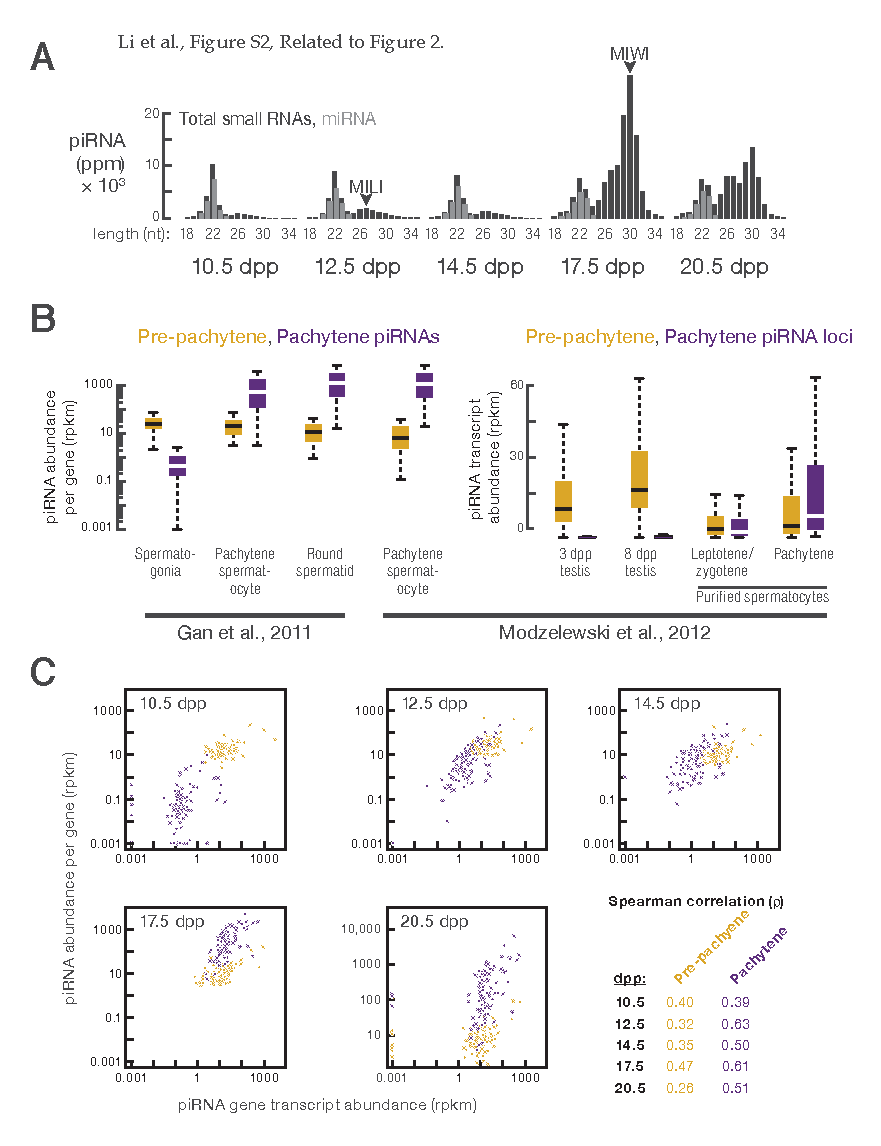
\includegraphics{Figures/MolCel/MolCel2013_FigS2.eps}
      \caption[Pre-pachytene piRNAs Persist in Pachytene Spermatocytes]
      {
        See subsection \ref{MolCel:subsubsection:cap:Figure S2} for full figure caption.
     	  }
      \label{MolCel:fig:MolCelS2}
      \end{figure}

    A parallel analysis of piRNA precursor transcription using RNA-seq (>100 nt) corroborated the classification based on piRNA abundance; of the 100 piRNA genes classified as pachytene based on the developmental expression profile of their piRNAs, 93 were grouped as pachytene according to the developmental expression profile of their transcripts. Of these 93, 89 are intergenic. All 84 piRNA genes designated pre-pachytene using piRNA data were classified as pre-pachytene according to their transcript abundance.

    Despite their name, pre-pachytene piRNAs were readily detected in >90\% and \textasciitilde95\% pure pachytene spermatocytes, as well as round spermatids (Figure \ref{MolCel:fig:MolCelS2}B; \citep{Gan2011,Modzelewski2012}. Transcript abundance from the 84 pre-pachytene loci was high at 3 dpp (median abundance = 11 rpkm), higher by 8 dpp (18 rpkm), and lower in purified leptotene/zygotene spermatocytes (3.3 rpkm; \ref{MolCel:fig:MolCelS2}B). Yet piRNA precursor transcripts were readily detectable in purified pachytene spermatocytes at a level (4.6 rpkm) comparable to that in purified leptotene/zygotene spermatocytes (Figure \ref{MolCel:fig:MolCelS2}B);  \citep{Gan2011,Modzelewski2012}. From 10.5 to 20.5 dpp, the steady-state level of pre-pachytene piRNA precursor transcripts remained constant (Figure \ref{MolCel:fig:MolCelS2}B).

    Finally, the abundance of pre-pachytene piRNA precursor transcripts was better correlated with pre-pachytene piRNA abundance at 17.5 dpp ($\rho$ = 0.47), when pachytene spermatocytes compose a larger fraction of the testis, than at 10.5, 12.5, or 14.5 dpp (0.32 $\ge \rho \le$ 0.40; Figure \ref{MolCel:fig:MolCelS2}C). Our data suggest that the pre-pachytene loci continue to be transcribed and processed into piRNAs long after spermatocytes enter the pachytene stage of meiosis. Thus, the name pre-pachytene piRNA is a misnomer that should be retained only for historical reasons.

    Hierarchical clustering identified 100 pachytene genes whose piRNAs emerge at 12.5 dpp, 2 days earlier than previously reported \citep{Girard2006}. Nearly all the pachytene genes are intergenic (93 out of 100). piRNA expression from pachytene piRNA genes peaks at 17.5 dpp (Figure \ref{MolCel:fig:MolCelF2}B). Overall, the median abundance of piRNAs from these 100 loci increased >6,000-fold from 10.5 to 17.5 dpp. Transcripts from pachytene genes were low at 10.5 dpp (median abundance = 0.15 rpkm) and increased 116-fold from 10.5 to 17.5 dpp. From 10.5 to 20.5 dpp, the dynamics of pachytene piRNA abundance from each piRNA gene correlated with the increase in abundance of its precursor transcripts (0.39 $\ge \rho \le$  0.63; $\rho value \le 7.3 x 10-5$; Figure \ref{MolCel:fig:MolCelS2}C). The 100 pachytene genes account for 92\% of piRNAs in the adult testis, making it unlikely that biologically functional pachytene piRNAs originate from thousands of genomic loci \citep{Gan2011}. Figures \ref{MolCel:fig:MolCelF3} and \ref{MolCel:fig:MolCelS3} provide examples of pachytene and pre-pachytene piRNA genes defined by our data.

    \begin{landscape}
    \begin{figure} % Figure 3
      \centering 
      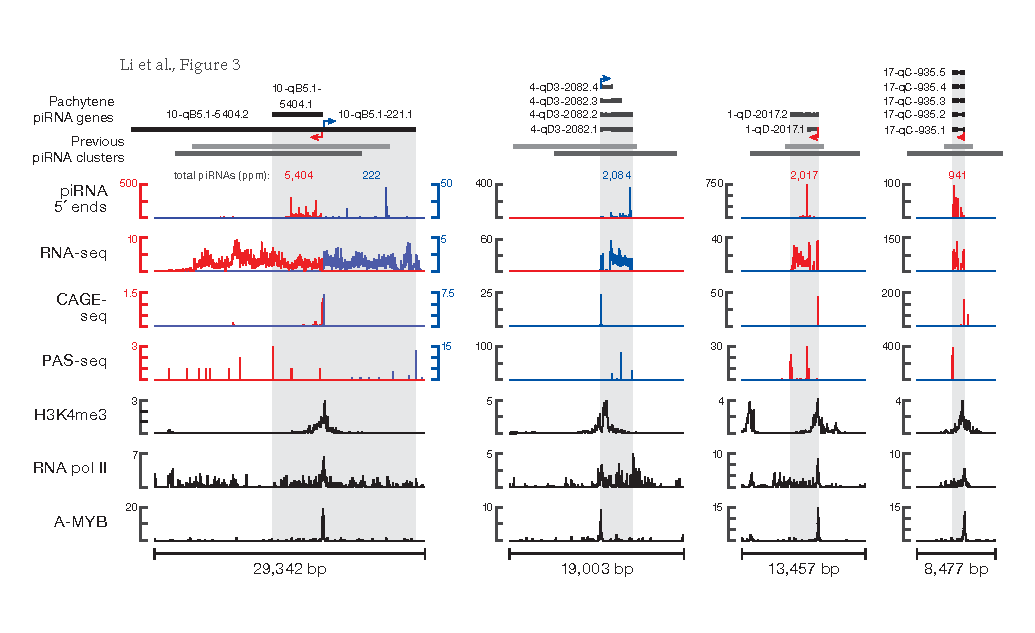
\includegraphics{Figures/MolCel/MolCel2013_Fig3.eps}
      \caption[Examples of Pachytene piRNA Genes]
      {
	      Previous cluster boundaries are from \citet{Lau2006} in gray and \citet{Girard2006} in  dark gray).
      	}
     	\label{MolCel:fig:MolCelF3}
   		\end{figure}

    \begin{figure} % Figure S3
      \centering 
      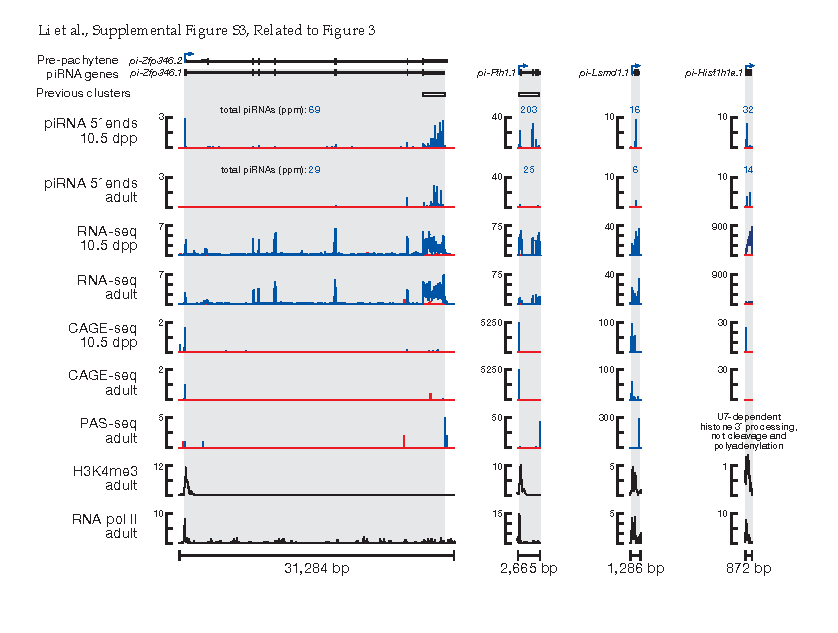
\includegraphics{Figures/MolCel/MolCel2013_FigS3.eps}
      \caption[Examples of Pre-Pachytene piRNA Genes]
      {
      	Previous cluster boundaries are from \citet{Lau2006} in gray and \citet{Girard2006} in  dark gray).
      	}
      \label{MolCel:fig:MolCelS3}
    	\end{figure}
    \end{landscape}

    Hierarchical clustering detected a third class, hybrid piRNAs, which derives from 30 genes with characteristics of both pre-pachytene and pachytene piRNA loci. Like pre-pachytene, hybrid piRNAs were detected at 10.5 dpp (median abundance = 3.7 rpkm) and in purified spermatogonia \citep{Gan2011}. Like pachytene piRNAs, hybrid piRNA abundance increased during the pachytene stage of meiosis, but the increase was delayed until late (17.5 dpp) rather than early pachynema (14.5 dpp). Overall, piRNAs from hybrid genes increased >10-fold from 14.5 to 17.5 dpp. The median abundance of piRNAs from hybrid piRNA genes ranged from 90-120 rpkm in purified pachytene spermatocytes, >20-fold greater than their median abundance in spermatogonia \citep{Gan2011,Modzelewski2012}. Moreover, hybrid piRNA precursor transcripts were readily detected in purified pachytene spermatocytes (median abundance = 9.0 rpkm; \citep{Modzelewski2012}).

    \subsubsection{Caption for Figure \ref{MolCel:fig:MolCelF2}}
      \label{MolCel:subsubsection:cap:Figure F2}
      (A) Normalized piRNA density (rpkm) for each piRNA-producing gene is shown as a heatmap across the developmental stages. Hierarchical clustering divided the genes into three classes. Arrowheads mark seven pachytene piRNA genes that were not classified as pachytene according to the change in the abundance of their precursor RNAs from 10.5 to 17.5 dpp.(B) Top: box plots present piRNA density per gene as spermatogenesis progresses (here and elsewhere, pre-pachytene in yellow and pachytene in purple). Middle: expression of \amyb{}, \bmyb{}, \mili{}, and \miwi{} was measured by RNA-seq. Bottom: box plots present piRNA precursor expression per gene, measured by RNA-seq, from 10.5 to 20.5 dpp. See also Figure \ref{MolCel:fig:MolCelS2} and Table S2.

    \subsubsection{Caption for Figure \ref{MolCel:fig:MolCelS2}}
      \label{MolCel:subsubsection:cap:Figure S2}
      (A) As shown previously by others using lower temporal resolution, the modal length of piRNAs increases as spermatogenesis proceeds to more advanced stages. (B) Total piRNA rpkm abundance and piRNA transcript abundance per locus by class, from purified spermatogonia, spermatocytes, round spermatids, and 3 dpp and 8 dpp testis \citep{Gan2011, Modzelewski2012}. (C) Correlation between piRNA abundance per locus and piRNA precursor transcription from 10.5 to 20.5 dpp. Throughout the Figures, gold indicates pre-pachytene and purple indicates pachytene piRNA loci.

  \subsection{\amyb{} Regulates Pachytene piRNA Precursor Transcription}
    \label{MolCel:subsec:A-Myb controls Pachytene precursor Tx}

    The coordinated increase in pachytene piRNA precursor transcripts suggests their regulation by a common transcription factor or factors. Among the 100 pachytene piRNA genes, 15 pairs (30 genes) are divergently transcribed. The 5\textprime~ends of the piRNA precursor RNAs from each pair are close in genomic distance (median = 127 bp), suggesting that a shared promoter lies between the two transcription start sites.
     
    We took advantage of the unique genomic organization of these 15 pairs of divergently transcribed piRNA genes to search for sequence motifs common to their promoters. The MEME algorithm \citep{Bailey1994} revealed a motif highly enriched in these bidirectional promoters (E = 8.3 x 10$^{12}$; Figure \ref{MolCel:fig:MolCelF4}A). This motif matches the binding site of the Myb family of transcription factors (Figure \ref{MolCel:fig:MolCelF4}A; \citep{Gupta2007, Newburger2009}. The Myb motif is not restricted to bidirectional promoters; MEME identified the same motif using the promoters of all pachytene piRNA genes (E = 9.1 x 10$^{-28}$; Figure \ref{MolCel:fig:MolCelF4}B).

    \begin{figure} % Figure 4
      \centering 
      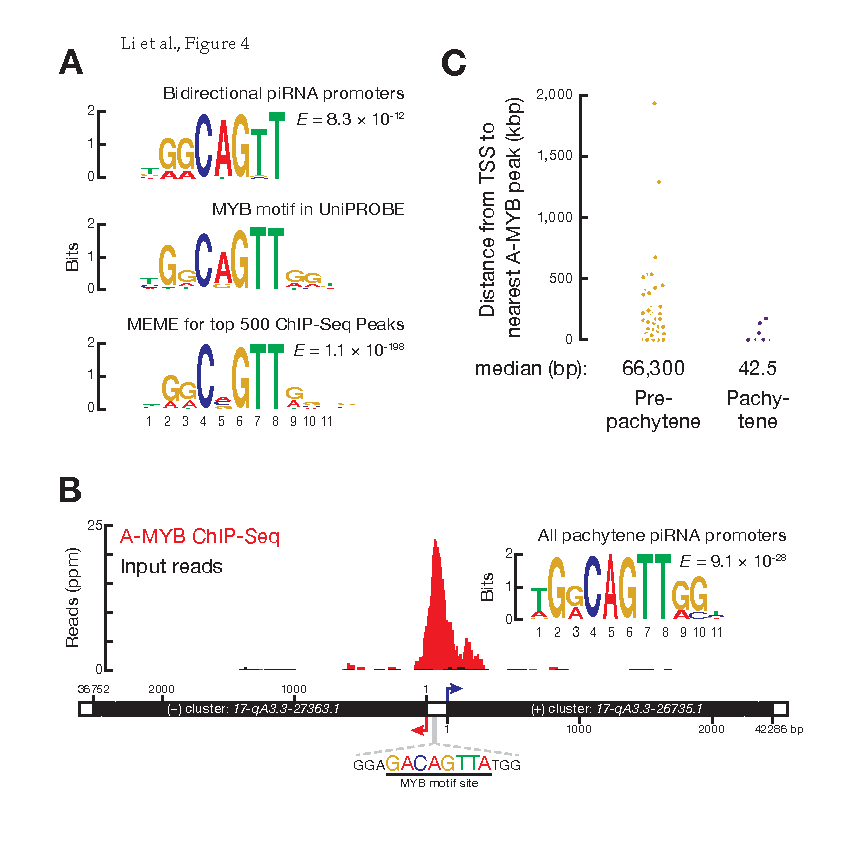
\includegraphics{Figures/MolCel/MolCel2013_Fig4.eps}
      \caption[A-MYB Binds the Promoters of Pachytene piRNA Genes]
      {
       (A) Top: MEME identified a sequence motif in the bidirectional promoters of the 15 pairs of divergently transcribed pachytene piRNA genes. E value computed by MEME measures the statistical significance of the motif. Middle: Myb motif from the mouse UniPROBE database. Bottom: MEME-reported motif for the top 500 (by peak score) A-MYB ChIP-seq peaks from adult mouse testes.(B) A-MYB ChIP-seq data for the common promoter of the divergently transcribed pachytene piRNA genes \textit{17-qA3.3-27363.1} and \textit{17-qA3.3-26735.1}.(C) The distance from the annotated transcription start site (TSS) of each piRNA gene to the nearest A-MYB peak. See also Figure \ref{MolCel:fig:MolCelS4}.
      	}
      \label{MolCel:fig:MolCelF4}
    	\end{figure}
    \begin{figure} % Figure S4
      \centering 
      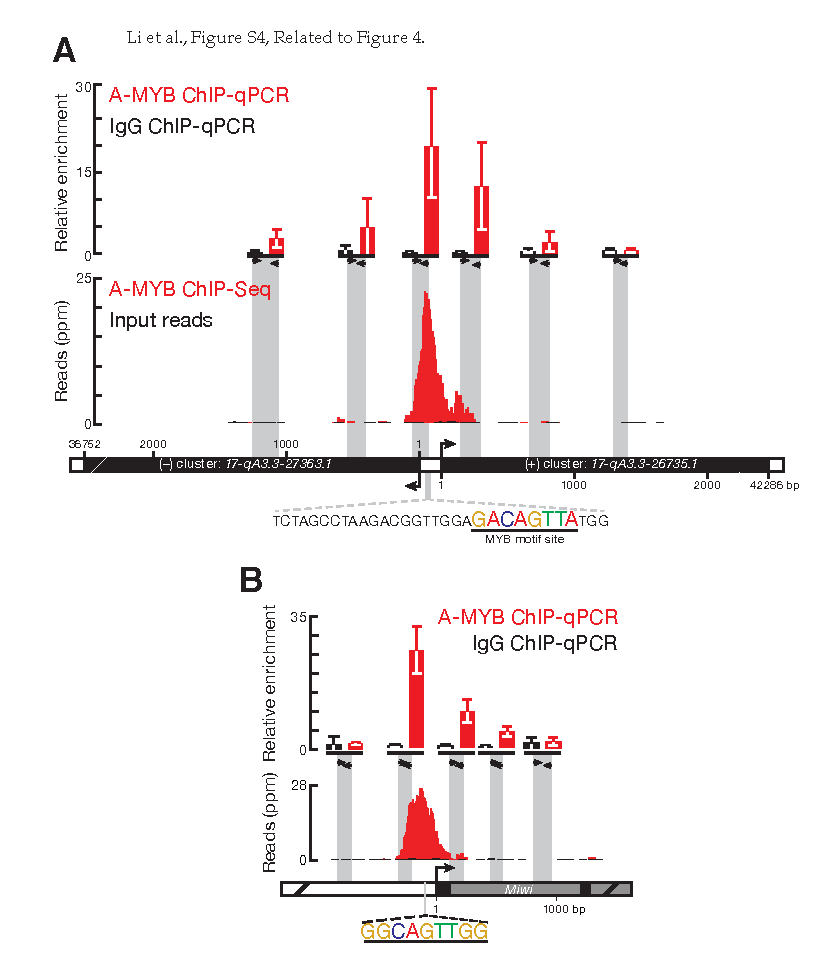
\includegraphics{Figures/MolCel/MolCel2013_FigS4.eps}
      \caption[ChIP-qPCR Confirms ChIP-seq Data]
      {
     	 (A) A-MYB binds to the common promoter of divergently transcribed pachytene piRNA loci \textit{17-qA3.3-27363.1} and \textit{17-qA3.3-26735.1}. The abundance of DNA fragments at the amplified region relative to a control region (mean $\pm$ standard deviation; n = 3) was measured by qPCR (top). The A-MYB ChIP-seq (red) and input (black) data for this pair of genes is presented as in Figure \ref{MolCel:fig:MolCelF4}B. (B) ChIP-seq and qPCR were as in (A), but for the promoter region of \miwi{} (Piwil1). Also shown is the RefSeq gene model. Exons, black; introns, gray.
     	 }
      \label{MolCel:fig:MolCelS4}
    	\end{figure}

    The Myb transcription factor family is conserved among eukaryotes. Like other vertebrates, mice produce three Myb proteins, A-MYB (MYBL1), B-MYB (MYBL2), and C-MYB (MYB), each with a distinct tissue distribution \citep{Mettus1994, Trauth1994, Latham1996, Oh1999}. Testes produce both A- and B-MYB proteins. Multiple lines of evidence implicate A-MYB, rather than B-MYB, as a candidate for regulating pachytene piRNA transcription. First, the expression of \amyb{} during spermatogenesis resembles that of pachytene piRNAs: \amyb{} transcripts appear at \textasciitilde12.5 dpp and peak at 17.5 dpp (Figure \ref{MolCel:fig:MolCelF2}B; \citep{Bolcun-Filas2011}. The expression of \amyb{} messenger RNA (mRNA) increases \textasciitilde15-fold from 8 dpp to 19 dpp, whereas \bmyb{} mRNA expression remains constant and low during the same time frame and into adulthood \citep{Horvath2009}. Our RNA-seq data (Figure \ref{MolCel:fig:MolCelF2}B) corroborate these findings. Indeed, in our RNA-seq analysis of adult testes, \amyb{} mRNA was 24-fold more abundant than \bmyb{}. Second, a testis-specific \amyb{} point-mutant allele, \mybrepro, which is caused by a cytosine-to-adenine transversion that changes alanine 213 to glutamic acid, leads to meiotic arrest at the pachytene stage with subtle defects in autosome synapsis; \amyb{} null mutant mice have defects in multiple tissues, including the testis and the mammary gland \citep{Toscani1997, Bolcun-Filas2011}. Third, our RNA-seq analysis of \amyb{} mutant testes shows that there is no significant change in \bmyb{} expression in the mutant, compared to the heterozygous controls, at 14.5 or 17.5 dpp. Finally, B-MYB protein is not detectable in pachytene spermatocytes \citep{Horvath2009}.

    To assess more directly the role of A-MYB in pachytene piRNA precursor transcription, we used anti-A-MYB antibody to perform ChIP followed by high-throughput sequencing of the A-MYB-bound DNA. The anti-A-MYB antibody is specific for A-MYB, and the peptide used to raise the antibody is not present in B-MYB. The model-based analysis of ChIP-seq (MACS) algorithm \citep{Zhang2008} reported 3,815 genomic regions with significant A-MYB binding (false discovery rate, FDR < 10$^{25}$); we call these regions A-MYB peaks or peaks. Among the 500 peaks with the lowest FDR values, 394 (80\%) contained at least one significant site ($\rho < 10^{4}$) for the MYB binding motif (Figure \ref{MolCel:fig:MolCelF4}A). Figure \ref{MolCel:fig:MolCelF4}B shows an example of such an A-MYB peak at the bidirectional promoter of the divergently transcribed pair of pachytene piRNA genes \textit{17-qA3.3-27363.1} and \textit{17-qA3.3-26735.1}. A-MYB occupancy of this genomic site was confirmed by ChIP and quantitative PCR (ChIP-qPCR) (Figure \ref{MolCel:fig:MolCelS4}A).

    The median distance from the transcription start site to the nearest A-MYB peak was \textasciitilde43 bp for the 100 pachytene piRNA genes but >66,000 bp for the 84 pre-pachytene genes (Figure \ref{MolCel:fig:MolCelF4}C). Our data suggest that during mouse spermatogenesis A-MYB binds to the promoters of both divergently and unidirectionally transcribed pachytene piRNA genes.

    To test the idea that A-MYB promotes transcription of pachytene, but not pre-pachytene, piRNA genes, we used RNA-seq to measure the abundance of RNA > 100 nt long from the testes of \amyb{} point-mutant (\mybrepro) mice and their heterozygous littermates (Figure \ref{MolCel:fig:MolCelF5}). Pachytene piRNA precursor transcripts—both divergently and unidirectionally transcribed—were significantly depleted in \amyb{} mutant testes compared to the heterozygotes: the median decrease was 45-fold at 14.5 dpp (q = 1.1 x 10$^{-13}$) and 248-fold at 17.5 dpp (q = 3.9 x 10$^{-23}$). The abundance of pre-pachytene piRNA transcripts was not significantly changed (q $\ge $ 0.34). The binding of A-MYB to the promoters of pachytene piRNA genes, together with the depletion of pachytene piRNA transcripts in the \amyb{} mutant, further supports the view that A-MYB directly regulates transcription of pachytene piRNA genes.

  \subsection{\amyb{} Regulates Pachytene piRNA Production}
    \label{MolCel:subsec:A-Myb regulates pachytene piRNA production}

    To test the consequences of the loss of piRNA precursor transcripts, we measured piRNA abundance in the \amyb{} mutant. Like pachytene piRNA precursor transcription, pachytene piRNA abundance significantly decreased in mutant testes. At 14.5 dpp, median piRNA abundance per pachytene gene decreased 87-fold in \amyb{} homozygous mutant testes compared to heterozygotes ($\rho < 2.2 X 10^{-16}$; Figure \ref{MolCel:fig:MolCelF5}. By 17.5 dpp, median pachytene piRNA abundance was >9,000 times lower in the \amyb{} mutant than the heterozygotes (P < 2.2 x 10$^{-16}$). In contrast, pre-pachytene piRNA levels were essentially unaltered. Figure 6 presents examples of the effect at 14.5 and 17.5 dpp of the \amyb{} mutant on piRNA precursor transcript and mature piRNA abundance for one pre-pachytene and three pachytene piRNA genes.

    \begin{figure} % Figure 5
      \centering 
      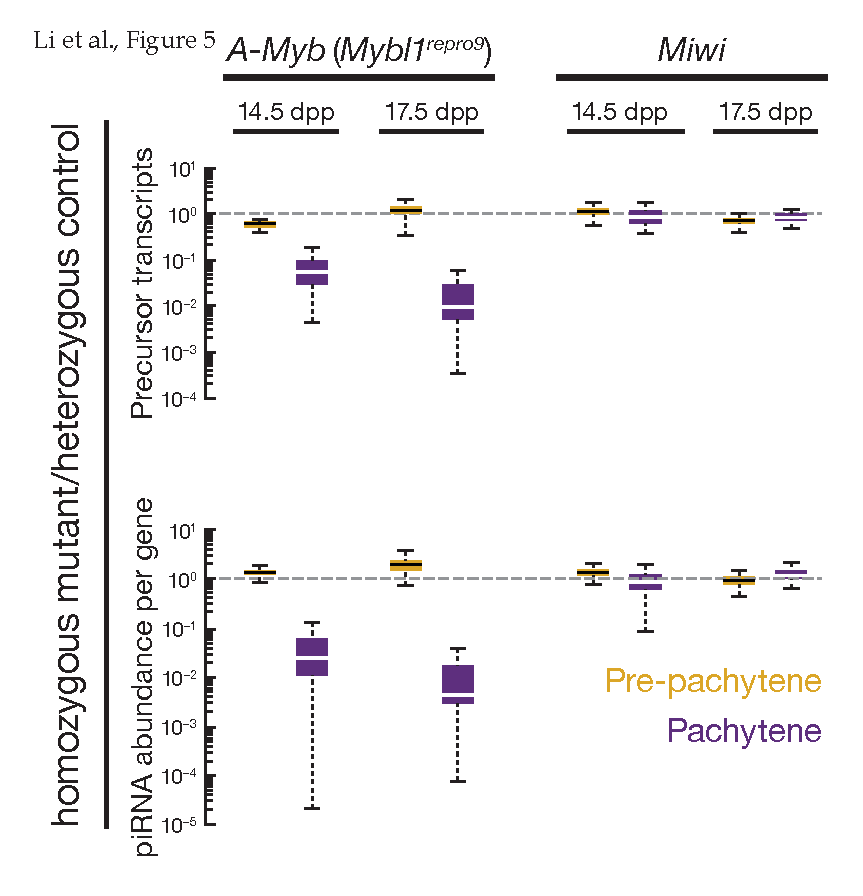
\includegraphics{Figures/MolCel/MolCel2013_Fig5.eps}
      \caption[Pachytene piRNAs and Precursors Decrease in \amyb{} Mutant Testes]
      {
     	 The change in transcript or piRNA abundance per gene in \amyb{} (n = 3) and \miwi{} (n = 1) mutants compared to heterozygotes in testes isolated at 14.5 and 17.5 dpp. See also Figure \ref{MolCel:fig:MolCelS5}.
     	 }
      \label{MolCel:fig:MolCelF5}
   	  \end{figure}
    \begin{figure} % Figure S5
      \centering 
      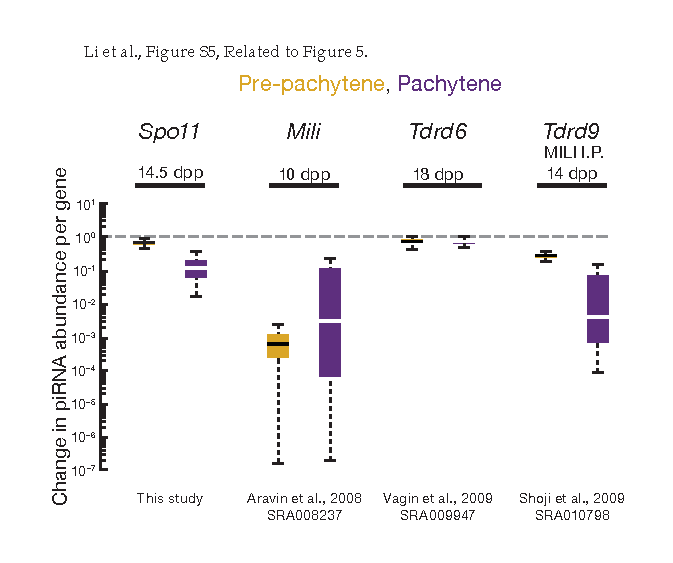
\includegraphics{Figures/MolCel/MolCel2013_FigS5.eps}
      \caption[Change in piRNA Expression in \spo{}, \miwi{}, \textit{Tdrd6}, and \textit{Tdrd9} Mutants]
      {
      Change in piRNA abundance per locus (rpkm) for \spo{} (14.5 dpp), \miwi{} (\textit{Piwil2}; 10.5 dpp), \textit{Tdrd6} (18 dpp), and \textit{Tdrd9} (14 dpp) mutants compared to heterozygous controls.
      }
      \label{MolCel:fig:MolCelS5}
 	   \end{figure}

    Our data show that A-MYB binds to the promoters of pachytene piRNA genes; \amyb{}, \miwi{}, and pachytene piRNA precursor transcription begins at 12.5 dpp; and \amyb{} mutant spermatocytes reach pachynema with subtle defects in autosome synapsis \citep{Bolcun-Filas2011}. Could pachytene piRNA depletion nonetheless be an indirect consequence of the meiotic arrest caused by the \amyb{} mutant? To test this possibility, we sequenced small RNAs from \spo{} mutant testes, which failed to generate double-stranded DNA breaks at the leptotene stage and display a meiotic arrest \citep{Baudat2000c,Romanienko2000}. The median abundance of piRNAs from pre-pachytene genes did not decrease at 14.5 dpp. By 17.5 dpp, piRNA from pachytene genes decreased just 5.9-fold in the \spo{} mutant testes compared to the heterozygotes (Figure \ref{MolCel:fig:MolCelS5}). We note that A-MYB protein abundance is reduced in the \spo{} mutant \citep{Bolcun-Filas2011}.

    \textit{Trip13} is required to complete the repair of double-strand DNA breaks on fully synapsed chromosomes. \textit{Trip13} mutants display a meiotic arrest similar to that in \amyb{} mutant testes \citep{Li2007}: pachytene arrest with synapsed chromosomes. To further test whether the loss of pachytene piRNA precursor transcripts in \amyb{} mutants reflects a general effect of meiotic arrest, we measured piRNA precursor transcript abundance in \textit{Trip13} mutant testes at 17.5 dpp. Unlike \amyb{}, piRNA precursor transcripts were readily detectable in the \textit{Trip13} mutant (Figure \ref{MolCel:fig:MolCelS6}). We conclude that the loss of pachytene piRNA precursor transcripts and piRNAs in \amyb{} mutant testes is a direct consequence of the requirement for A-MYB to transcribe pachytene piRNA genes and not a general feature of meiotic arrest at the pachytene stage.

  \subsection{\amyb{} Regulates Expression of piRNA Biogenesis Factors}
    \label{MolCel:subsec:A-Myb regulations piRNA machinery}

    The \amyb{} mutant more strongly affected pachytene piRNA accumulation than it did the steady-state abundance of the corresponding piRNA precursor transcripts (Figure \ref{MolCel:fig:MolCelF5}; the median decrease in pachytene piRNA abundance was 2-fold greater at 14.5 dpp and 38-fold greater at 17.5 dpp than the decrease in the steady-state abundance of pachytene precursor transcripts (Table S1). These data suggest that A-MYB exerts a layer of control on piRNA accumulation beyond its role in promoting pachytene piRNA precursor transcription.

    \miwi{} has previously been proposed to be a direct target of A-MYB; \miwi{} mRNA abundance is reduced in A-MYB mutant testes, and ChIP microarray data place A-MYB on the \miwi{} promoter \citep{Bolcun-Filas2011}. Our RNA-seq data confirm that accumulation of \miwi{} mRNA requires A-MYB: \miwi{} mRNA decreased more than 50-fold in testes isolated from \amyb{} mutant mice at 14.5 dpp compared to their heterozygous littermates (Figures \ref{MolCel:fig:MolCelF7}A and \ref{MolCel:fig:MolCelS7} and Table S3). Furthermore, our ChIP data confirm that A-MYB binds the \miwi{} promoter in vivo (Figures \ref{MolCel:fig:MolCelF7}B, \ref{MolCel:fig:MolCelS4}B, and \ref{MolCel:fig:MolCelS7}). Like pachytene piRNAs, \miwi{} transcripts first appear at 12.5 dpp (Figure \ref{MolCel:fig:MolCelF2}B), and MIWI protein is first detected in testes at 14.5 dpp \citep{Deng2002c}. Loss of MIWI arrests spermatogenesis at the round spermatid stage \citep{Deng2002c}.

    A previous study reported that piRNAs fail to accumulate to wild-type levels in \miwi{} mutant testes \citep{Grivna2006}. However, our data suggest that the overall change in piRNA abundance caused by loss of MIWI is quite small: RNA-seq detected no change at 14.5 dpp (change in total piRNA abundance = 1.1; n = 2) and only a modest decrease at 17.5 dpp (change in total piRNA abundance = 0.58; n = 1). piRNAs from pachytene loci decreased just 2.7-fold at 14.5 dpp (p = 0.0046) and 3.5-fold at 17.5 dpp (p = 1.8 x 10-6) in \miwi{} mutant testes (Figure \ref{MolCel:fig:MolCelF5}). By comparison, pachytene piRNAs declined 87-fold at 14.5 dpp and 9,400-fold at 17.5 dpp in the \amyb{} mutant.

    Does the loss of MIWI affect piRNA precursor transcription? We measured transcript abundance and piRNA expression in \miwi{} null mutant testes at 14.5 and 17.5 dpp. In \miwi{}$^{-/-}$ testes, pachytene piRNA precursor transcripts were present at levels indistinguishable from \miwi{} heterozygotes (median change = 1.0- to 1.4-fold; q = 1; Figure \ref{MolCel:fig:MolCelF5}). Thus, loss of MIWI does not explain loss of pachytene piRNA precursor transcripts in \amyb{} mutant testes.

    \begin{figure} % Figure 6
      \centering 
      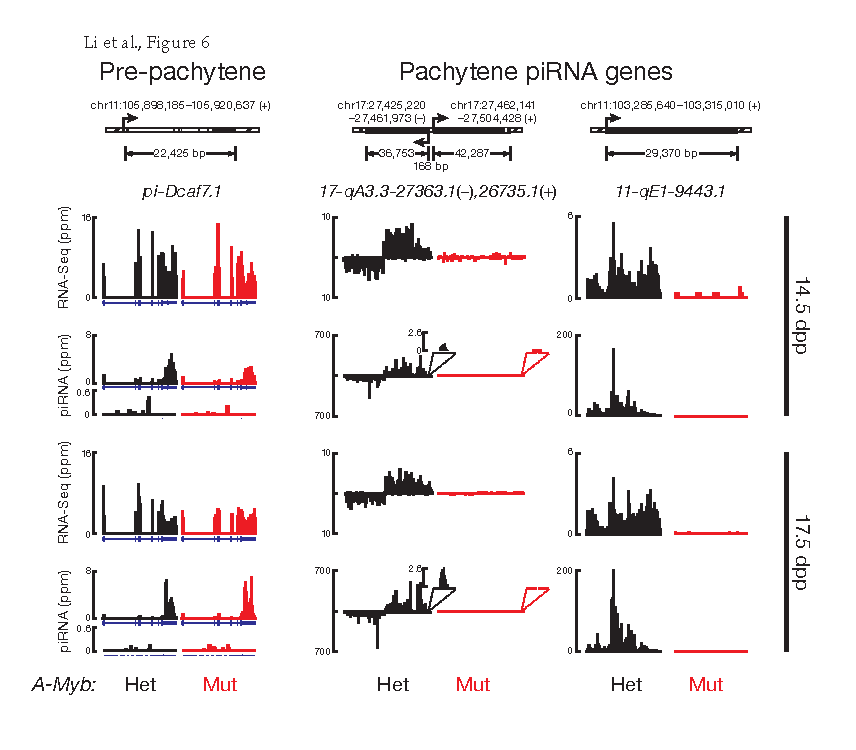
\includegraphics{Figures/MolCel/MolCel2013_Fig6.eps}
      \caption[Examples of the Effect of the \amyb{} Mutation on piRNA Expression]
      {
     	 Transcript and piRNA abundance in heterozygous (Het) and homozygous \amyb{} (Mut) point-mutant testes is shown for four illustrative examples at 14.5 and 17.5 dpp. Also shown is the abundance of piRNA sequencing reads that map to the exon-exon junctions. Gene \textit{11-qE1-9443} does not have an intron. Exons, blue boxes; splice junctions, gaps; the last exon is compressed and not to scale. See also Figure \ref{MolCel:fig:MolCelS6}.
     	 }
      \label{MolCel:fig:MolCelF6}
    	\end{figure}
    \begin{figure} % Figure S6
      \centering 
      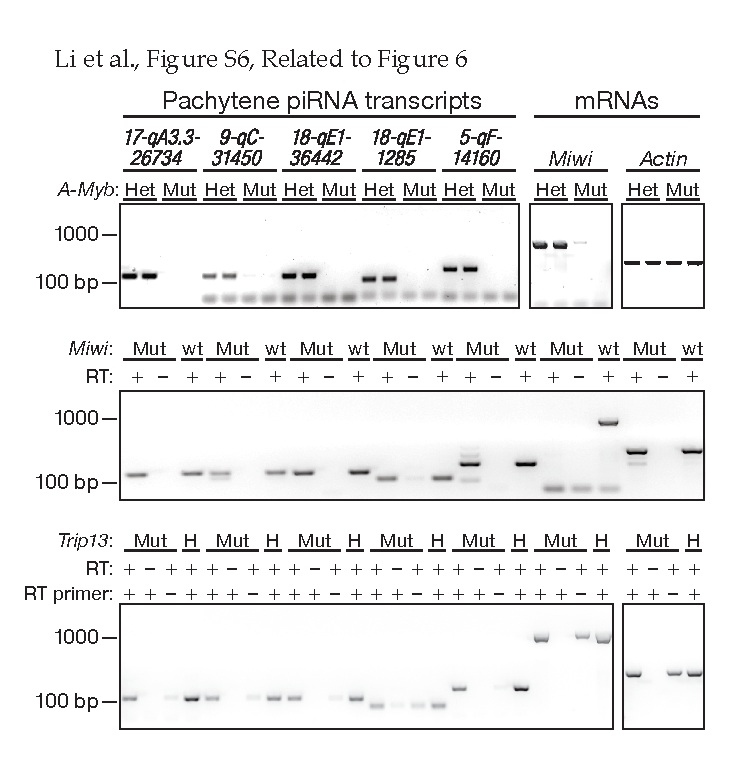
\includegraphics{Figures/MolCel/MolCel2013_FigS6.eps}
      \caption[Pachytene piRNA Precursor Abundance in \amyb{}, \miwi{}, and \textit{Trip13} Mutants]
      {
      Transcripts were detected in total RNA from adult testes by RT-PCR (using random primers) for five pachytene piRNA loci as well as \miwi{} and \textit{Actin}. Mut, mutant; Het or H, heterozygote; wt, wild type.
      }
      \label{MolCel:fig:MolCelS6}
   	  \end{figure}

    In addition to \miwi{}, ChIP-seq detected A-MYB bound to the promoters of 12 other RNA-silencing-pathway genes (Figure \ref{MolCel:fig:MolCelF7}B and Table S3). Of these, the mRNA abundance—measured by three biologically independent RNA-seq experiments—of \textit{Ago2}, \textit{Ddx39} (uap56 in flies), \textit{Mael}, \mili{}, \textit{Mov10l1}, \textit{Tdrd9}, and \textit{Vasa} did not change significantly at 14.5 dpp in \amyb{} mutant testes compared to heterozygotes (q > 0.05); except for \textit{Ago2}, all decreased significantly in the mutant at 17.5 dpp. In contrast, the abundance of the mRNAs encoding Tudor domain proteins decreased significantly in \amyb{} mutant testes: \textit{Tdrd6} (64-fold decrease; q = 3.1 x 10-5) and \textit{Tdrd5} (7.5-fold decrease; q = 1.0 x 10-5). \textit{Tdrd5} is expressed in embryonic testes then decreases around birth \citep{Yabuta2011}. \textit{TDRD5} protein reappears at 12 dpp, increasing throughout the pachynema \citep{Smith2004, Yabuta2011}. Our data indicate that A-MYB activates \textit{Tdrd5} transcription at the onset of the pachytene stage of meiosis. Similarly, \textit{Tdrd6} mRNA can be detected at the middle pachytene, but not the zygotene stage, and peaks after late pachytene; TDRD6 protein can be detected at 17 dpp and continues to increase until 21 dpp \citep{Vasileva2009}. The findings that TDRD5 and TDRD6 colocalize with MIWI in pachytene spermatocytes \citep{Hosokawa2007, Vasileva2009, Yabuta2011} and that TDRD6 binds MIWI \citep{Chen2009a, Vagin2009, Vasileva2009} suggest a role for these Tudor domain proteins in pachytene piRNA production or function. As in \miwi{}-/- testes, spermatogenesis arrests at the round spermatid stage in \textit{Tdrd5}$^{-/-}$ and \textit{Tdrd6}$^{-/-}$ mutant testes \citep{Vasileva2009, Yabuta2011}. Loss of \textit{Tdrd6} expression has little effect on piRNA levels (Figure \ref{MolCel:fig:MolCelS3}; \citep{Vagin2009}, perhaps because the functions of Tudor domain proteins overlap.

    Other genes encoding piRNA pathway proteins whose promoters are bound by A-MYB and whose expression decreased significantly in \amyb{} mutant testes include \textit{MitoPld} (\textit{Pld6}; 3.9-fold decrease; q = 0.0095) and \textit{Tdrd12} (5.3-fold decrease; q = 0.0046). \textit{MitoPld} encodes an endoribonuclease implicated in an early step in piRNA biogenesis in mice and flies \citep{Houwing2007, Pane2007, Haase2010, Huang2011, Watanabe2011a, Ipsaro2012, Nishimasu2012}. The function of Tdrd12 is not known, but its fly homologs (Yb, Brother of Yb, and Sister of Yb) are all required for piRNA production \citep{Handler2011}. \textit{Tdrd1} decreased 3.4-fold, but with q value = 0.015. \textit{Tdrd1} is first expressed in fetal prospermatogonia, then re-expressed in pachytene spermatocytes \citep{Chuma2006a}. In Tdrd1 mutant testes, spermatogenesis fails, with no spermatocytes progressing past the round spermatid stage \citep{Chuma2006a}. TDRD1 binds MILI and MIWI \citep{Chen2009a, Kojima2009} and colocalizes with TDRD5 and TDRD6 in the chromatoid body \citep{Hosokawa2007}.

    Together, these data support the idea that at the onset of the pachytene phase of meiosis, A-MYB coordinately activates transcription of many genes encoding piRNA pathway proteins.

  \subsection{A-MYB and the Pachytene piRNA Regulatory Circuitry}
    \label{MolCel:subsec:A-MYB and piRNA regulatory circuitry}

    A number of genes encoding known and suspected piRNA pathway proteins are bound and regulated by A-MYB (Figures \ref{MolCel:fig:MolCelF7}B and \ref{MolCel:fig:MolCelS7}C). Our data support a model in which A-MYB drives both the transcription of pachytene piRNA genes and the mRNAs encoding genes required for piRNA production including \miwi{}, \textit{MitoPld}, and \textit{Tdrd9}. Regulation by A-MYB of both the sources of pachytene piRNAs and the piRNA biogenesis machinery creates a coherent feedforward loop (Figure \ref{MolCel:fig:MolCelF7}C). Feedforward loops amplify initiating signals to increase target gene expression. Furthermore, they function as switches that are sensitive to sustained signals; they reject transient signals \citep{Shen-Orr2002, Osella2011}. 

    A-MYB also bound to the \amyb{} promoter (Figure \ref{MolCel:fig:MolCelF7}B), and \amyb{} transcripts decreased 4.2-fold in testes from an \amyb{} point mutant (\mybrepro{}; Figure \ref{MolCel:fig:MolCelF7}B). The \amyb{} mutant fails to produce the high level of A-MYB protein observed in wild-type testes at the late pachytene stage of meiosis \citep{Bolcun-Filas2011}. Instead, A-MYB protein never becomes more abundant than the level achieved in wild-type testes by the beginning of the pachytene stage. While the lower level of A-MYB in the \amyb{} mutant may reflect instability of the mutant protein, a simpler explanation is that mutant A-MYB cannot activate \amyb{} transcription.

    \begin{figure} % Figure 7
      \centering
      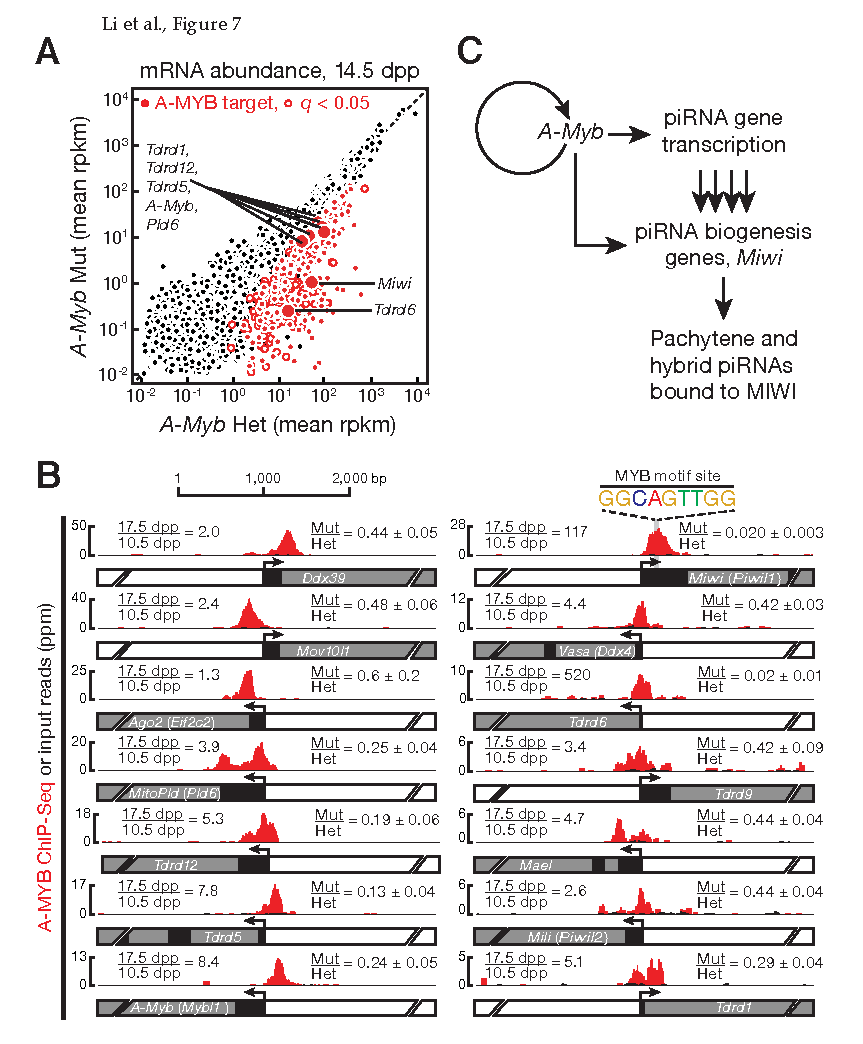
\includegraphics{Figures/MolCel/MolCel2013_Fig7.eps}
      \caption[A-MYB Regulates Expression of mRNAs Encoding piRNA Pathway Proteins]
      {
        See subsubsection \ref{MolCel:subsubsection:cap:Figure F7} for full figure caption.
      	}
      \label{MolCel:fig:MolCelF7}
    	\end{figure}

    \begin{figure} % Figure S7
      \centering 
      \includegraphics{Figures/MolCel/MolCel2013_FigS7.eps}
      \caption[\amyb{} mutants, but Not \miwi{} Mutants, Change the Expression of RNA Silencing Pathway Genes]
      {
      	See subsubsection \ref{MolCel:subsubsection:cap:Figure S7} for full figure caption.
      	}
      \label{MolCel:fig:MolCelS7}
    	\end{figure}

      \subsubsection{Caption for Figure \ref{MolCel:fig:MolCelF7}}
        \label{MolCel:subsubsection:cap:Figure F7}
        (A) mRNA abundance in \amyb{} mutant versus heterozygous testes. The 407 genes with a significant (q < 0.05) change in steady-state mRNA levels are shown as red circles. The 203 with A-MYB peaks within 500 bp of their transcription start site are filled.
        (B) A-MYB ChIP-seq signal at the transcription start sites of \amyb{} and genes implicated in RNA silencing pathways. For each, the figure reports the change in mRNA abundance between 17.5 and 10.5 dpp in wild-type testes and the mean change between \amyb{} mutant and heterozygous testes at 14.5 dpp (mean $\pm$ SD; n = 3).
        (C) A model for the regulation of pachytene piRNA biogenesis by A-MYB. See also Figure \ref{MolCel:fig:MolCelS7} and Table S3.

      \subsubsection{Caption for Figure \ref{MolCel:fig:MolCelS7}}
        \label{MolCel:subsubsection:cap:Figure S7}
        A) mRNA abundance in 17.5 dpp \amyb{} versus heterozygous testes. The 2,853 genes with a significant (q < 0.051) change in steady-state mRNA abundance are shown as open red circles. Among them, 8721,009 genes also had A-MYB peaks within 500 bp of their transcription start sites. These ``A-MYB targets'' are marked with filled red circles. (B) Same as (A) but in 14.5 dpp \miwi{} mutant versus heterozygous testes. The genes encoding proteins implicated in RNA silencing pathways that were labeled in (A) and that showed no change in expression in \miwi{} mutant testes are highlighted as green filled circles. As expected, \miwi{}, showed a significant decrease in mRNA abundance in \miwi{}-/- testes. (C) The change in mRNA abundance (rpkm) in \amyb{} and \miwi{} mutant testes versus heterozygous controls for the RNA silencing genes highlighted in (A) and (B).

  \subsection{Feed-Forward Regulation of piRNA Production is Evolutionarily Conserved}
    \label{MolCel:subsec:A-MYB in Chickens}

    Is A-MYB-mediated, feedforward control a general feature of regulation of piRNA production among vertebrates? To test whether A-MYB control of piRNA precursor transcription is evolutionarily conserved, we used high-throughput sequencing to identify piRNAs in adult rooster testes. Birds and mammals diverged 330 million years ago \citep{Benton2007}. After removing the sequences of identifiable miRNAs \citep{Burnside2008} and annotated noncoding RNAs, total small RNA from the adult rooster testis showed peaks at both 23 and 25 nt (Figure \ref{MolCel:fig:MolCelF8}A). When the RNA was oxidized before being prepared for sequencing, only a single 25 nt peak remained, consistent with the 25 nt small RNAs corresponding to piRNAs containing 2\textprime-O-methyl-modified 3\textprime~termini. These longer, oxidation-resistant species typically began with uracil (62\% of species and 65\% of reads; Figure \ref{MolCel:fig:MolCelF8}B), and we detected a significant Ping-Pong amplification signature (Z score = 31; Figure \ref{MolCel:fig:MolCelF8}C). We conclude that the oxidation-resistant, 24-30 nt long small RNAs correspond to rooster piRNAs. Like piRNAs generally, rooster piRNAs are diverse, with 5,742,529 species present among 81,121,893 genome-mapping reads. Like mouse pachytene piRNAs, 70\% of piRNAs from adult rooster testes mapped to unannotated intergenic regions, 19\% mapped to transposons, and 14\% mapped to protein-coding genes. Of the piRNAs that map to protein-coding genes, >95\% derive from introns. Forty-two percent of piRNA species mapped uniquely to the Gallus gallus genome.

    Using 24-30 nt piRNAs from oxidized libraries, we identified 327 rooster piRNA clusters (Figure \ref{MolCel:fig:MolCelS8}). These account for 76\% of all uniquely mapping piRNAs. Of the 327 clusters, 25 overlapped with protein-coding genes. To begin to identify the transcription start sites for the rooster piRNA clusters, we analyzed adult rooster testes by H3K4me3 ChIP-seq. More than 81\% (268 out of 327) of the clusters contained a readily detectable H3K4me3 peak within 1 kbp of the piRNA cluster. In contrast, the median distance from a cluster to the nearest transcription start site of an annotated gene was 73 kbp, suggesting that the H3K4me3 peaks reflect the start sites for rooster piRNA precursor transcripts.

    Next, we asked where in the genome A-MYB bound in adult rooster testes. A-MYB ChIP-seq identified 5,509 significant peaks (FDR < 10-25). MEME analysis of the top 500 peaks with the lowest FDR values identified a motif (E = 2.6 x 10-201; Figure \ref{MolCel:fig:MolCelF8}D) similar to that found in the mouse (Figure \ref{MolCel:fig:MolCelF4}A). A-MYB is the only one of the three chicken MYB genes expressed in adult testis (X.Z.L. and P.D.Z., unpublished data), supporting the view that these peaks correspond to A-MYB binding. The core sequence motif associated with A-MYB binding in mouse differs at one position (CAGTT) from that in rooster (C C/G GTT). This difference between mammalian and chicken MYB proteins has been noted previously \citep{Weston1992, Deng1996}.


    \begin{figure} % Figure 8
      \centering 
      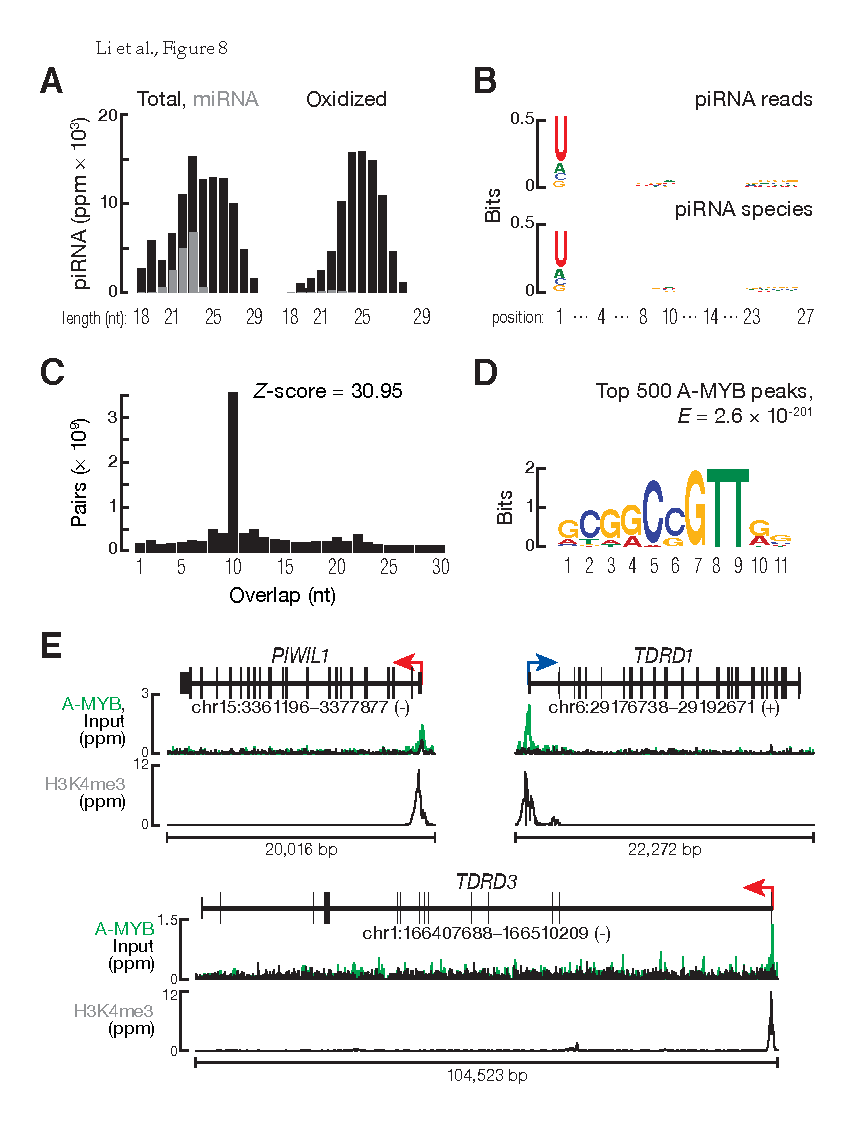
\includegraphics{Figures/MolCel/MolCel2013_Fig8.eps}
      \caption[Feed-Forward Regulation of piRNA Biogenesis by A-MYB is Conserved in Rooster]
      {
        See subsubsection \ref{MolCel:subsubsection:cap:Figure F8} for full figure caption.
      	}
      \label{MolCel:fig:MolCelF8}
    	\end{figure}
    \begin{figure} % Figure S8
      \centering 
      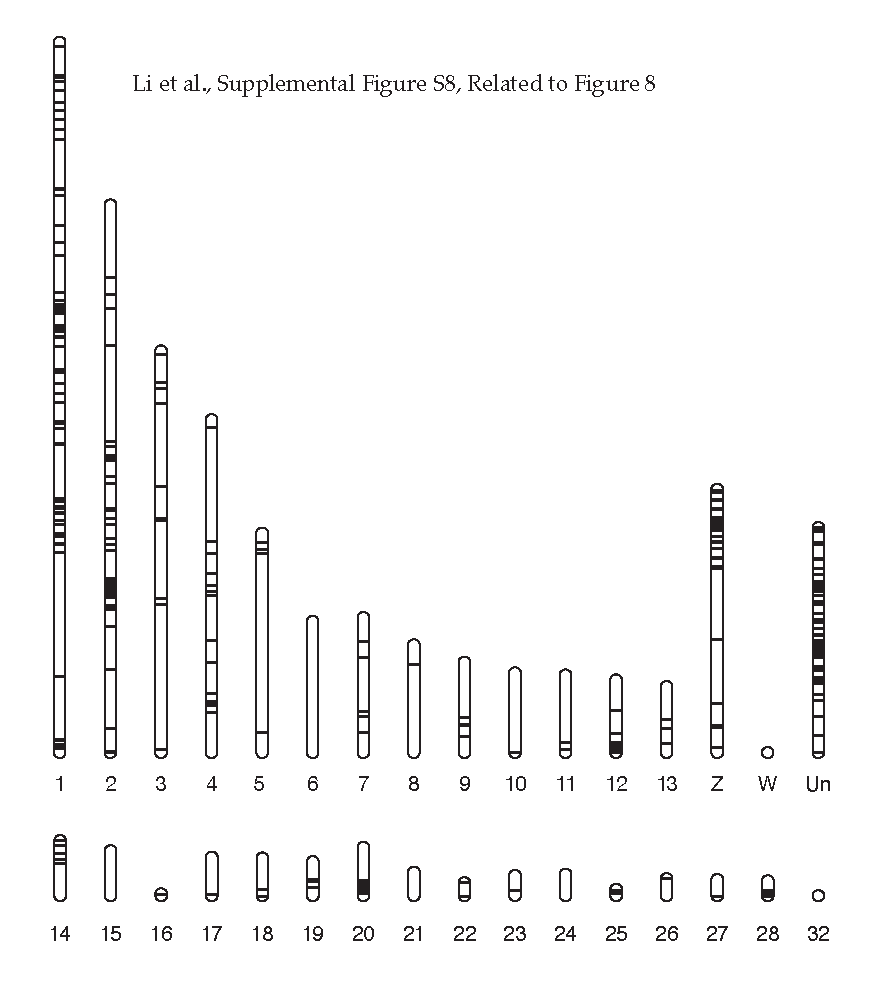
\includegraphics{Figures/MolCel/MolCel2013_FigS8.eps}
      \caption[Genomic Locations of piRNA Clusters in the Rooster (Gallus gallus) Testis.]
      {
     	 Black horizontal lines denote the locations on the Gallus gallus (galGal3) chromosomes of the piRNA clusters identified by small RNA sequencing. The figure shows 324 clusters; clusters on E64 (cluster 370) and E22C19W28_E50C23 (clusters 109 and 563) are not shown.
     	 }
      \label{MolCel:fig:MolCelS8}
    	\end{figure}

    To determine whether chicken A-MYB might regulate transcription of some piRNA clusters in the testis, we compared the A-MYB peak nearest to each piRNA cluster with the nearest H3K4me3 peak. Of the 327 rooster piRNA clusters, at least 104 were occupied by A-MYB at their promoters, as defined by an overlapping H3K4me3 peak. These 104 clusters account for 31\% of uniquely mapping rooster piRNAs.

    The chicken genome encodes at least two PIWI proteins: PIWIL1 and PIWIL2. Remarkably, the promoter of Gallus gallus PIWIL1, the homolog of mouse \miwi{}, contained a prominent A-MYB peak (Figure \ref{MolCel:fig:MolCelF8}E). TDRD1 and TDRD3 also showed A-MYB peaks (Figure \ref{MolCel:fig:MolCelF8}E). Thus, as in mice, Gallus gallus A-MYB controls the transcription of both piRNA clusters and genes encoding piRNA pathway proteins. We conclude that A-MYB-mediated feedforward regulation of piRNA production was likely present in the last common ancestor of birds and mammals.

    In mice, we found no piRNA-producing genes on the sex chromosomes (Figure \ref{MolCel:fig:MolCelS1}A), perhaps because mouse sex chromosomes are silenced during the pachytene stage \citep{Li2009d}. Birds use a ZW rather than an XY mechanism for sex determination, so roosters are homogametic (ZZ), allowing the sex chromosomes to remain transcriptionally active in males \citep{Namekawa2009, Schoenmakers2009}. Indeed, we find that 39 of the 327 rooster piRNA clusters are on the Z chromosome, accounting for 12\% of uniquely mapping piRNAs (Figure \ref{MolCel:fig:MolCelS8}). Of the 39 Z chromosome clusters, 18 had an A-MYB peak at their promoter.

    \subsubsection{Caption for figure \ref{MolCel:fig:MolCelF8}}
    \label{MolCel:subsubsection:cap:Figure F8}
      (A) Length distributions of total rooster testis small RNAs (black) and miRNAs (gray).(B) Sequence logo showing the nucleotide composition of piRNA reads and species.(C) The 5\textprime~-5\textprime~overlap between piRNAs from opposite strands was analyzed to determine if rooster piRNAs display Ping-Pong amplification. The number of pairs of piRNA reads at each position is reported. Z score indicates that a significant 10 nt overlap (Ping-Pong) was detected. Z score > 1.96 corresponds to p value < 0.05.(D) MEME-reported motif of the top 500 (by peak score) A-MYB ChIP-seq peaks from adult rooster testes.(E) A-MYB, H3K4me3, and input ChIP-seq signals at the transcription start sites of rooster PIWIL1, TDRD1, and TDRD3. See also Figure S8.

\section{Discussion}
  \label{MolCel:sec:Discussion}

  The data presented here provide strong support for the view that piRNAs in mammals begin as long, single-stranded precursors generated by testis-specific, RNA Pol II transcription of individual piRNA genes (see also \citet{Vourekas2012}. Transcription by RNA Pol II affords piRNA genes the same rich set of transcriptional controls available to regulate mRNA expression. Our data establish that developmentally regulated transcription of piRNA genes determines when specific classes of piRNAs emerge during spermatogenesis.

  During mouse spermatogenesis, transcription of pachytene piRNA genes begins at the onset of the pachytene stage of meiosis; pachytene piRNAs accumulate subsequently. The presence of the MYB binding motif near the transcription start sites of pachytene piRNA genes, the physical binding of A-MYB to those genes, and the loss of pachytene piRNA precursor transcripts and piRNAs in testes from \amyb{} mutant mice all argue that A-MYB regulates pachytene piRNA production.

  A-MYB also drives increased expression of piRNA pathway genes. Among these, \miwi{} expression shows the greatest dependence on A-MYB, but A-MYB also drives transcription of genes encoding other proteins in the piRNA pathway, including MitoPld, Mael, and five genes encoding Tudor domain proteins. For example, A-MYB increases expression of Tdrd6 more than 500-fold. Loss of A-MYB function more strongly depletes pachytene piRNAs than loss of MIWI, in part because pachytene piRNAs can still be loaded into MILI in \miwi{} mutant testes, although MILI-loaded pachytene piRNAs do not suffice to produce functional sperm. In the \amyb{} mutant, expression of mRNAs encoding multiple piRNA pathway proteins decreases. We speculate that in wild-type male mice, the increased expression of these mRNAs at the onset of the pachytene stage of meiosis ensures that sufficient piRNA-precursor-processing and MIWI-loading factors are available to cope with the large increase in pachytene piRNA precursor transcription.

  We propose that induction of A-MYB during the early pachytene stage of spermatogenesis initiates a feedforward loop that ensures the precisely timed production of these piRNAs. Coherent feedforward loops show delayed kinetics in order to reject background stimuli \citep{Mangan2003}. Indeed, we observed a delay from the early to middle pachytene in the accumulation of pachytene piRNAs, despite the continued increase in \amyb{} expression (Figure \ref{MolCel:fig:MolCelF2}A). Pachytene piRNA levels increase 75-fold (median for the 100 genes) from 10.5 to 12.5 dpp, coincident with increased expression of \amyb{}. However, from 12.5 to 14.5 dpp, pachytene piRNAs increase only 1.2-fold. Pachytene piRNAs subsequently resume their accumulation, increasing 65-fold from 14.5 to 17.5 dpp. We believe this delay is a consequence of a feedforward loop that ensures the production of pachytene piRNAs only at the pachytene stage of spermatogenesis. Regulation by a feedforward loop also predicts a rapid shutdown of pachytene piRNA pathways at round spermatid stage VIII, when A-MYB protein levels decrease \citep{Horvath2009}. Supporting this idea, the abundance of MIWI decreases sharply by the elongated spermatid stage of spermatogenesis \citep{Deng2002c}. Testing this proposal is a clear challenge for the future.

  In fruit flies and zebrafish \citep{Brennecke2007, Houwing2007}, most piRNAs map to repetitive regions, whereas in mammals, uniquely mapping intergenic piRNAs predominate in the adult testis. The discovery that 70\% of rooster piRNA reads map to intergenic regions suggests that the expansion of intergenic piRNAs controlled by A-MYB feedforward regulation arose before the divergence of birds and mammals. In the future, detailed analysis of piRNA production across avian spermatogenesis should provide insight into the evolutionary origins and functions of pachytene piRNAs, a class of piRNAs thus far only detected in mammals.

  In summary, we have shown that mouse piRNA genes are coregulated transcriptionally, establishing that A-MYB coordinately regulates the biogenesis of an entire piRNA class, the pachytene piRNAs. The discovery that a loss-of-function \amyb{} mutant, \mybrepro{}, disrupts piRNA precursor transcription in vertebrates provides a tool to understand the transformation of long, single-stranded piRNA precursors into mature piRNAs and to explore the functions and targets of the pachytene piRNAs.

\section{Experimental Procedures}
  \label{MolCel:sec:Experimental Procedures}

  \begin{description}
    \item[Mice] \hfill \\
    \mybrepro{}, \textit{\spo{}}$^{tm1Sky}$, and \textit{Piwil1}$^{tm1Hf}$ mice were maintained and used according to the guidelines of the Institutional Animal Care and Use Committee of the University of Massachusetts Medical School and genotyped as described \citep{Baudat2000c, Deng2002c, Bolcun-Filas2011}.

    \item[Sequencing] \hfill \\
    Small \citep{Ghildiyal2008, Seitz2008} and long RNA-seq \citep{Zhang2012a} and analysis \citep{Li2009a} were as described. Reads that did not map to mouse genome mm9 were mapped to piRNA precursor transcripts to obtain splice junction mapping small RNAs. Total small RNA libraries from different developmental stages and from mutants were normalized to the sum of all miRNA hairpin mapping reads. Oxidized samples were calibrated to the corresponding total small RNA library via the abundance of shared, uniquely mapped piRNA species. piRNA expression data were grouped with Cluster 3.0. Differential gene expression was analyzed with DESeq R \citep{Anders2010a}; ChIP-seq reads were aligned to the genome using Bowtie version 0.12.7 \citep{Langmead2009}, and peaks were identified using MACS \citep{Zhang2008}.

    \item[Acknowledgments] \hfill \\
    We thank K. Chase and K. Schimenti for help collecting tissues; C. Tipping for help with mouse husbandry; P. Johnson and B. Keagle for providing rooster testes; G. Farley for technical assistance; H. Lin for reagents; Xi Chen, Xiaotu Ma, Oliver Rando, and Benjamin Carone for advice on ChIP; and members of our laboratories for critical comments on the manuscript. X.Z.L. was supported by the Lalor Foundation and the Jane Coffin Childs Memorial Fund for Medical Research.

    \item[Accession Numbers] \hfill \\
    The Gene Expression Omnibus (GEO) accession number for the RNA-seq, ChIP-seq, and small RNA data reported in this paper is GSE44690.

    \item[Animals] \hfill \\
    Mice were maintained and used according to the guidelines of the Institutional Animal Care and Use Committee of the University of Massachusetts Medical School. C57BL/6J (Jackson Labs, Bar Harbor, ME, USA; stock number 664); \mybrepro{} in a mixed 129X1/SvJ x C57BL/6J background; Spo11tm1Sky in a C57BL/6J background; and Piwil$^{1tm1Hf}$ in a mixed 129X1/SvJ x C57BL/6J background (``\miwi{}'') mice were genotyped as described \citep{Baudat2000c, Deng2002c, Bolcun-Filas2011}. Rooster testes from White Leghorn of the Cornell Special C strain, about 15 months old, were used for small RNA analysis; and testes from the Brown Leghorn strain, about one year old, were used for ChIP analysis.

    \item[RNA Sequencing] \hfill \\
    Small RNA libraries were constructed and sequenced as described \citep{Ghildiyal2008, Seitz2008} except that 18-35 nt RNA was isolated and 2S rRNA depletion omitted. Sequencing was performed using either a Genome Analyzer GAII (36 or 76 nt reads) or HiSeq 2000 (50 nt) instrument (Illumina, San Diego, CA, USA). We analyzed published small RNA libraries from purified mouse spermatogonia (SRR069809), spermatocytes (SRR069810, GSE39652), or spermatids (SRR069811; \citep{Gan2011, Modzelewski2012}; from \mili{} mutant or heterozygous testes at 10 dpp (SRX003089 and SRX003088; \citep{Aravin2008a}; from Tdrd6 mutant or heterozygous testes at 18 dpp (SRX012165 and SRX012166; \citep{Vagin2009}; and MILI IP samples from Tdrd9 mutant or heterozygous testes at 14 dpp (SRX015795, SRX015796, SRX015797, and SRX015798; \citep{Shoji2009}.

    Strand-specific RNA-seq libraries \citep{Zhang2012} using Ribo-Zero Gold (Epicentre Biotechnologies, Madison, WI, USA) were sequenced using the paired-end protocol on a HiSeq 2000.
    
    \item[Small RNA Analysis] \hfill \\
    Small RNA sequence analysis was as described \citep{Li2009a} using mouse genome release mm9 and chicken genome release galGal3. Non-coding RNA annotations comprised data from ncRNAscan, the known tRNAs from UCSC, and 18S, 28S and 5.8S rRNAs. miRNA hairpin and mature miRNA annotation was from miRBase Release 19. Mouse and chicken transposons were annotated using Repeat Masker from UCSC. Reads that did not map to the mouse genome (mm9) were mapped to piRNA precursor transcripts to obtain splice junction-mapping small RNAs. Total small RNA libraries from different developmental stages and from mutants were normalized to the sum of all miRNA hairpin-mapping reads. Oxidized samples were calibrated to the corresponding total small RNA library via the abundance of shared, uniquely mapped piRNA species. Table S1 reports the statistics for high-throughput sequencing. For oxidized (i.e., piRNA-enriched) samples, uniquely mapping small RNAs >23 nt were mapped to each assembled piRNA precursor transcript and reported as reads per kilobase pair per million reads mapped to the genome (rpkm) using a pseudo count of 0.001.

    \item[Small RNA Analysis] \hfill \\
    RNA-seq reads were aligned to the genome (NCBI 37/mm9) using TopHat 2.0.4 \citep{Trapnell2009}. Reads were mapped uniquely using the ``-g 1'' switch. We assembled the mouse testes transcriptome (see below). For genes with multiple isoforms, the transcript with the highest average rpkm value among the three replicates of adult testes was selected for further analysis. Fragments with both reads mapped within a transcript, or to piRNA precursor transcripts, were counted using BEDTools \citep{Quinlan2010}. The sum of the reads aligning to the top quartile of expressed transcripts per library was used to calibrate the samples. The number of reads per transcript was normalized by length, divided by the library-specific calibration factor, and reported as rpkm with a pseudo count of 0.001. Table S1 presents the statistics for the RNA-seq data. Sequences mapping to five genes (Table S1) that overlapped with or were embedded within a piRNA gene were excluded when calculating piRNA precursor transcript abundance.

    \item[PAS-seq Library Construction and Analysis] \hfill \\
    PAS-seq libraries (Table S1) were prepared essentially as described \citep{Shepard2011} and sequenced using a HiSeq 2000 (100 nt read length). We first removed adaptors and performed quality control using Flexbar 2.2 (http://sourceforge.net/projects/theflexibleadap) with the parameters ``-at 3 -ao 10 --min-readlength 30 --max-uncalled 70 --phred-pre-trim 10.'' For reads beginning with GGG including (NGG, NNG or GNG) and ending with three or more adenosines, we removed the first three nucleotides and mapped the remaining sequence with and without the tailing adenosines to the mouse genome using TopHat 2.0.4. We retained only those reads that could be mapped to the genome without the trailing adenosine residues. Genome-mapping reads containing trailing adenosines were regarded as potentially originating from internal priming and thus discarded. The 3\textprime~end of the mapped, retained read was reported as the site of cleavage and polyadenylation.

    \item[CAGE Library Construction and Analysis] \hfill \\
    CAGE (cap analysis of gene expression; Table S1) was as described \citep{Yang2011} and sequenced using a HiSeq 2000 (100 nt reads). After removing adaptor sequences and checking read quality using Flexbar 2.2 with the parameters of 
    \lstset{language=BASH}
    \begin{lstlisting}
    -at 3 -ao 10 --min-readlength 20 --max-uncalled 70 --phred-pre-trim 10
    \end{lstlisting}
    , we retained only reads beginning with NG or GG (the last two nucleotides on the 5\textprime~adaptor). We then removed the first two nucleotides and mapped the sequences to the mouse genome using TopHat 2.0.4. All unique 5\textprime~ends of the mapped positions were considered as CAGE-tag starting sites and grouped into tag clusters using a distance-based method in which the maximal distance between two neighboring tags was required to be <20 bp. The peak position of a tag cluster was then reported as the transcription start site.

    \item[Transcriptome Assembly and Annotation] \hfill \\
    De novo transcriptome assembly from three biological replicates of strand-specific RNA-seq data from adult testes was performed using Trinity (r2012-06-08) with default parameters \citep{Grabherr2011}. The assembled RNA sequences were aligned to the mouse genome (mm9) with BLAT \citep{Kent2002}, and the alignments with more than 95\% of sequence length mapped and fewer than 1\% mismatches retained.

    We extracted novel junctions from Trinity (i.e., reads with [0-9]+M[0-9]+N[0-9]+M pattern in the CIGAR string of SAM output), and re-mapped all RNA-seq reads to these junctions, rescuing 1,402,444 reads in three replicates. Rescued reads were combined with TopHat alignments (supplied with ``-max-multihits 100'' to assembly through repetitive regions) and used as input for reference-based assembly.

    We used Cufflinks v2.0.2 \citep{Trapnell2010} with parameters of:
    \lstset{language=BASH}
    \begin{lstlisting}
    -u -j 0.2 --min-frags-per-transfrag 40
    \end{lstlisting}
    to assemble transcripts. To join small transcript fragments caused by insufficient read coverage or embedded repetitive elements, two different gap-joining distance cutoffs were used for the assembly of genes (``\-\-overlap-radius 100'') and piRNA loci (``--overlap-radius 250''). We used Cuffcompare v2.0.2 \citep{Trapnell2010} to annotate the 49,840 Cufflinks-assembled transcripts using parameters optimized for genic conditions (``\-\-overlap-radius 100'').

    \item[piRNA Precursor Transcript Annotation] \hfill \\
    We combined transcripts from the two Cufflink assemblies with those from the Trinity assembly, producing 136,069 unique transcripts. Those transcripts with 100 ppm or 100 rpkm unique mapping piRNAs at any time point (10.5, 12.5, 14.5, 17.5, 20.5 dpp and adult oxidized small RNA from testis) were selected for manual annotation.

    To refine the termini of the piRNA-producing transcripts, we supplemented the RNA-seq data with high-throughput sequencing of 5\textprime~ends of RNAs bearing (5\textprime~)ppp(5\textprime~) cap structures (CAGE) and of the 3\textprime~ends of transcripts flanking the poly(A) tail (PAS-seq). To provide independent confirmation of the 5\textprime~ends of each piRNA-producing transcript, we used chromatin immunoprecipitation (ChIP-seq) of RNA polymerase II (pol II) and histone H3 bearing trimethylated lysine-4 (H3K4me3). Refinement of transcriptional starts required both a CAGE and a H3K4me3 peak to support the 5\textprime~end of the transcript. When no H3K4me3 peak corroborated alternative transcription start sites proposed by the CAGE data, the alternative transcripts were merged with the fully substantiated transcript.

    \item[piRNA Gene Nomenclature] \hfill \\
    When piRNA-producing genes overlap an annotated protein coding gene, we refer to them using the name of the overlapping gene preceded by ``pi-''; when they do not, their names refer to their genomic location followed by a number indicating the piRNA abundance in ppm at 6 weeks post-partum. The last digit of a piRNA gene name specifies the rank order of expression among isoforms, determined by the highest abundance of transcripts (rpkm) observed for that gene among the six developmental stages of testis.

    \item[Grouping piRNA Precursor Transcripts] \hfill \\
    For the most abundant transcript in each locus, the abundance (rpkm) of piRNAs at each stage was expressed as a fraction of the maximum abundance reached during the developmental time course. These data were then analyzed by hierarchical clustering according to Euclidean distance and complete linkage using Cluster 3.0. Clustering results were visualized using Java Tree View 1.1.3.

    \item[Analysis of Differential Gene Expression ] \hfill \\
    We determined differential gene expression using DESeq R \citep{Anders2010a}. For each annotated mRNA, reads from each library were aligned to the most abundant assembled transcript. Transcripts with q < 0.05 were considered to be differentially expressed. Table S3 lists the genes that were differentially expressed in \amyb{} at 14.5 dpp. Three biologically independent replicates were used for \amyb homozygotes and heterozygotes at 14.5 and at 17.5 dpp.

    \item[Motif Discovery] \hfill \\
    For divergently transcribed piRNA gene pairs, the promoter region was defined as the region between the transcription start sites defined by CAGE peaks. Sequence motifs in these putative promoter regions were detected ab initio using MEME \citep{Bailey1994, Bailey2009} in TCM mod (any number of repetitions per sequence) and compared to existing JASPAR and TRANSFAC libraries via TOMTOM \citep{Gupta2007}. FIMO was used to detect motif sites within the putative promoters (default p < 10$^{-4}$; \citep{Grant2011}.

    \item[Chromatin Immunoprecipitation (ChIP)] \hfill \\
    ChIP was performed as described \citep{Chen2008} except that testes were macerated on ice and then fixed with 1.5\% (w/v) formaldehyde for 20 min. Samples were then further crushed using 20 strokes with a ``B'' pestle in a Dounce homogenizer (Kimble-Chase, Vineland, NJ, USA). Chromatin was sheared by sonication and immunoprecipitated using anti-A-MYB (HPA008791; Sigma, St. Louis, MO, USA) or anti-H3K4me3 (ab8580; Abcam, Cambridge, MA, USA) antibody; immunoglobulin G (IgG; Sigma, item 2729) served as a control. ChIP-quantitative PCR (qPCR) was performed using the CFX96 Real-Time PCR Detection System with SsoFast EvaGreen Supermix (Bio-Rad, Hercules, CA, USA). Data were analyzed using DART-PCR \citep{Peirson2003}. Relative ChIP enrichment values were normalized to \textit{MyoD1}, a gene not expressed in testes. Table S1 lists ChIP-qPCR primers. ChIP-seq libraries for anti-A-MYB and control input DNA were prepared following the Illumina ChIP-seq protocol and sequenced on a HiSeq 2000 (50 nt reads).

    \item[ChIP-seq Analysis] \hfill \\
    ChIP-seq reads were aligned to the genome using Bowtie version 0.12.7 \citep{Langmead2009}. Reads were mapped uniquely using the ``-M 1 --best --strata'' switches and one mismatch was allowed (-v 1). ChIP peaks were identified using MACS version 1.4.1 \citep{Zhang2008} using default arguments, input as control, and a cutoff p-value = 10$^{-25}$ was used. BEDTools was used to assign peaks to the nearest 5\textprime~end of genes. Table S1 reports sequencing statistics for ChIP-seq.

    \item[RT-PCR] \hfill \\
    Total RNA was treated with Turbo DNase (Ambion, Austin, TX, USA), and then reverse transcribed using SuperScript III (Invitrogen, Eugene, OR, USA) with random primers (Promega, Madison, WI, USA). The resulting cDNA was analyzed by conventional PCR. Table S1 lists the primers used in Figure \ref{MolCel:fig:MolCelS6}.

    \item[Ping-Pong Analysis] \hfill \\
    Ping-Pong amplification was analyzed by the 5\textprime~-5\textprime~overlap between piRNA pairs from opposite genomic strands \citep{Li2009a}. Overlap scores for each overlapping pair were the product of the number of reads of each of the piRNAs from opposite strands. The overall score for each overlap extend (1-30) was the sum of all such products for all chromosomes. Heterogeneity at the 3\textprime~ends of small RNAs was neglected. Z-score for 10 bp overlap was calculated using the scores of overlaps from 1-9 and 11-30 as background.

    \item[Rooster piRNA Cluster Detection] \hfill \\
    We developed a dynamic programming algorithm to identify the genomic regions with the highest piRNA density. We used oxidized small RNA reads (>23 nt) to detect clusters. We used the conservative assumption that piRNA clusters compose at most 2\% of the chicken genome. We first split the genome into 1 kbp non-overlapping windows and computed piRNA abundance for each window. The mean of the top 2\% of windows was used as the penalty score for the dynamic programming algorithm. The algorithm computes the cumulative piRNA abundance score as a function of the window index along each chromosome. The score at a window is the sum of the score in the previous window and the piRNA abundance in the current window, minus the penalty score; if the resulting score was negative it was reset to 0. The maximal score points to the largest piRNA cluster. We extracted the largest piRNA cluster, recomputed the scores at the corresponding windows, and searched for the next cluster. The process continued until the scores for all windows were zero. The boundaries of each cluster were further refined by including those base pairs for which piRNA abundance exceeded the mean piRNA abundance of the top 2\% windows. We considered only those clusters with abundance >10 ppm for uniquely mapping piRNAs. In Figure \ref{MolCel:fig:MolCelF8}E, gene models were corrected using data from our unpublished adult rooster testis RNA-seq data.

  	\end{description}

\cleardoublepage
  % !TEX root = /Users/royc/Google_Drive/Thesis/RoyC_Umass_Thesis.tex
\chapter{SeqZip - Development and Applications} 
\label{SeqZipMethod} 
\lhead{Chapter 4. \emph{SeqZip - Development and Applications}} 
%----------------------------------------------------------------------------------------
\section{Overview}
  \label{SeqZipMethod:sec:SeqZip Overview}

  Development of SeqZip began with an attempt to circumvent an obvious shortcoming in second generation HTS---short read lengths. Until second generation HTS (i.e. reads <100nt on either the Illumina or SOLiD platforms), most sequencing was done using cloned fragments, stored in bacteria, and analyzed using dideoxy ``Sanger Sequencing'' (see \ref{Intro:subsec:DNA Sequencing History}). Indeed, this is how most \hyperref[hd:abrevs]{EST}s where analyzed. An extremely powerful feature of these ESTs is that as they represent the sequence of a single original molecule of RNA. Connectivity between sequences that were far apart (>1,000 nt) in the original sequence was maintained. It is this very feature, the continuity of sequence, that allowed whole genome shotgun sequencing to be used, and ESTs to be assembled into complete genomes, despite sometimes lengthly, repetitive, stretches of DNA (see section \ref{Intro:subsec:DNA Sequencing History}). Once research transitioned over to heavy use of the second generation HTS, all of that connectivity was lost, and all the inherent information with it.

  Second generation HTS can be supplemented with other technologies. This has been demonstrated perhaps most successfully with long-read assisted genome assembly \citep{Koren2012a}. Why not supplement the disconnected nature of short reads with another technology? To that end, Phillip D. Zamore proposed an RNA-templated DNA-DNA ligation approach as drawn in Figure \ref{SeqZipMethod:fig:Original SeqZip Diagram} (see US Patent application \href{http://1.usa.gov/PTG9BB}{12/906,678}). Using this approach, two or more distant sequences of RNA are investigated using short DNA oligonucleotides that force the intervening sequences to loop out. Incorporation of the hybridized DNA via ligation with those of DNAs adjacently hybridized generates a positive readout of sequence presence.

  \begin{figure} % Original SeqZip Diagram
    \centering 
    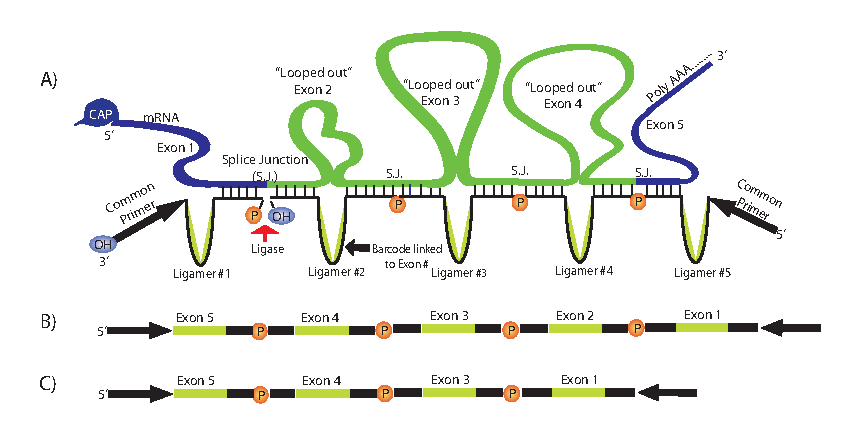
\includegraphics{Figures/SeqZipMethod/OriginalSeqZipDiagram.eps}
    \caption[Original SeqZip Diagram]
    {
      Original SeqZip Diagram\\[0.25cm]
      The original concept diagram of the SeqZip methodology. (A) Specific DNA oligos target an mRNA and loop out the RNA sequence. Ligases is added to join the DNA oligos together; (B) \& (C) Two different possibilities of ligation products templated from the RNA in (A), where Exon 2 is an cassette exon.
    	}
    \label{SeqZipMethod:fig:Original SeqZip Diagram}
  	\end{figure}

  Along with Patent \href{http://1.usa.gov/PTG9BB}{12/906,678}, Chapter \ref{SeqZipPaper} presents much of the early and important developmental work demonstrating reduction to practice of this method (termed ``SeqZip"), and its application to investigating connectivity of sequence content in the biologically-interesting genes \fn{} and \dscam{}. 

  Presented in this Chapter are experiments demonstrating SeqZip application to the following questions and issues:

  \begin{itemize} % Itemized list of sections
    \singlespacing
    \item Section \ref{SeqZipMethod:sec:Multiplex Gene Study}: 
      Simultaneous investigation of 10 genes ("Multiplex") for coordinated alternative splicing.
    \item Section \ref{SeqZipMethod:sec:RNA Integrity via SeqZip}: 
      Investigation of RNA integrity using SeqZip.
    \item Section \ref{SeqZipMethod:sec:piRNA precursor by SeqZip}: 
      Demonstrating the presence of long, continuous piRNA precusors by SeqZip
	  \end{itemize}

  The three sections add to the data discussed in Chapter \ref{SeqZipPaper} in some important ways. Section \ref{SeqZipMethod:sec:Multiplex Gene Study} demonstrates that SeqZip can not only be used to investigate an extremely complex alternatively spliced gene (\dscam{}) in a comprehensive manner, but can also be applied to looking at multiple genes at once. Section \ref{SeqZipMethod:sec:RNA Integrity via SeqZip} exploits a subtle feature of the method---that the RNA must be intact in order to produce a ligation product. This can be used to report on a fraction of intact RNA and deduce meaningful information such as the amount of intact RNA virus, or the existence of as-yet unobserved mega transcripts, like mammalian piRNA precursors (section \ref{SeqZipMethod:sec:Demonstrating continuous precursor TX by SeqZip}).

\section{Multiplex SeqZip Application}
  \label{SeqZipMethod:sec:Multiplex Gene Study}

  Is the coordination discussed in section \ref{Intro:subsec:Coordination in splicing} a general phenomenon? One of the major goals of developing SeqZip was to investigate potential coordination genome-wide. By genome-wide, what we really mean is to analyze many (or all) of the RNA transcripts in a tissue for evidence of coordinated splicing decisions. When development of the method reached the point that it could be applied to a multiplex study, I did not posses the bioinformatic skills necessary to (1) identify target transcripts, exons, and sequences to investigate for potential connectivity and (2) design ligamers in an automated and high-throughput fashion. Both of these points are discussed later (see \ref{SeqZipMethod:sec:Demonstrating continuous precursor TX by SeqZip} and \ref{Disc}).

  In order to make some progress on applying the technique to multiple genes at once, I used data presented by \citet{Fagnani2007}. This paper identified genes displaying tissue-specific splicing patterns, focusing on those with CNS-specific patterns. One section focused on ``Coordination between alternative splicing events belonging to the same genes,'' and seemed to be the exact type of genes we were interested in applying SeqZip too. Five hundred of the 3,044 genes investigated by their microarrays contained 2\textendash 5 alternative exons. \citet{Fagnani2007} contained an additional data file listing all pair-wise combinations of alternative exons in the same gene (with that gene having significant expression in >20 different tissues) along with the standard and partial spearman correlations. 

  It is important to note that the genes above also contain alternative first exons, a prominent type of alternative splicing (Figure \ref{Intro:fig:asEventsBarChart}). Indeed, from microarrays studies, it has been estimated that approximately 16\%\textendash 23\% of all alternative splicing events involve alternative first and last exons \citep{Bingham2008}. It is known that, through alternative use of first and last exons, cells can fine-tune a transcript's untranslated region (UTR) and control many aspects of mRNA regulation including nuclear export, localization, expression, and stability \citep{Hughes2006}.

  Using the \citet{Fagnani2007} data, I filtered exon pairs to those with a distance >350 nt between exons in the final pre-mRNA. I also visualized their transcript architecture, and EST evidence using NCBI's AceView tool \citep{Thierry-Mieg2006}. For example, the exons with strong correlation of expression in \textit{Chl1} are in the beginning (second exon) and end (fourth from last exon, accession BC060216) with plenty of supporting evidence for these exons being expressed and skipped. After combing through \citep{Fagnani2007} data, I assembled a list of 11 genes (Table \ref{table: BigSpanGenes}) to investigate for coordinated splicing.

  \begin{table} % Big Span Genes in mice from Fagnani 2007
    \caption[Mouse genes with large sequence between suggested coordinated cassette exons]
      {
        A list of 11 genes investigated in section \ref{SeqZipMethod:sec:Multiplex Gene Study}. Coordination between exons first suggested by \citep{Fagnani2007}.
        }
    \label{table: BigSpanGenes}
    \begin{table}[h]
\begin{tabular}{|l|r|r|r|r|}
\hline
\textbf{Gene name} & \textbf{nt of mRNA between exons} & \textbf{possible isoforms} & \textbf{Exon 1} & \textbf{Exon 2} \\ \hline
Chl1               & 4665                              & 18                         & 2               & 24              \\ \hline
Mdm1               & 1846                              & 4                          & EDA             & IIICS           \\ \hline
PTPRF-Y            & 1633                              & 4                          & 2               & 13              \\ \hline
Cacna1c            & 1403                              & 4                          & 15              & 21/22           \\ \hline
PTPRF-X            & 936                               & 4                          & 9/10            & 21              \\ \hline
FN1                & 813                               & 8                          & 13/14           & 21/22           \\ \hline
Apbb1              & 802                               & 260                        & 1/2b            & 2/3e            \\ \hline
Agrn               & 736                               & 8                          & 33/34c          & 33/34a          \\ \hline
Exoc7              & 513                               & 4                          & 7               & 13              \\ \hline
Prom1              & 512                               & 4                          & 7               & 9               \\ \hline
Lphn2              & 396                               & 32                         & 19              & 24/25a          \\ \hline
\end{tabular}
  \caption[Genes with big spans in between]{\hl{caption}}
  \label{table: BigSpanGenes}
\end{table}

    \end{table}

  I hand-designed ligamers for each of these genes. Ligamers were ordered from IDT in a 96-well plate format, pooled according to gene, and used to develop a multiplex approach to applying SeqZip. I used total RNA from mouse brains as the input material.

  After attempts to perform SeqZip on all 11 genes in one ligation failed, I reverted back to \textit{per-gene} ligation reactions in order to trouble shoot and optimize the assay. Once I had obtained ligation products from per-gene ligation reactions for both the individual and combination ligamers pools, I pooled all the ligation products and amplified them. Amplified products were sent for paired-end 100 sequencing on the Illumina GEIIx platform. 

  After considerable delay and optimization from the Umass Sequencing Core due to low library sequence diversity, the analyzed data demonstrated little alternative splicing in the genes examined. Put another way---most of the transcripts observed via SeqZip were uniform in exon inclusion and showed little variation for cassette exon inclusion (Figure \ref{SeqZipMethod:fig:Apbb1 Results}). These results forced us to rethink applying SeqZip to multiple genes or complex alternative splicing (i.e. \dscam{}). For most genes, there were too few reads aligning to combination products, arguing for more careful mixing of the more efficient individual products with lower-efficiency combination products prior to sequencing. For a discussion of different type of multiplex study, see section \ref{Disc:subsec: Ideal SeqZip exp. to look for Coordination}.

  \begin{figure} % Appb1 Multplex example
    \centering 
    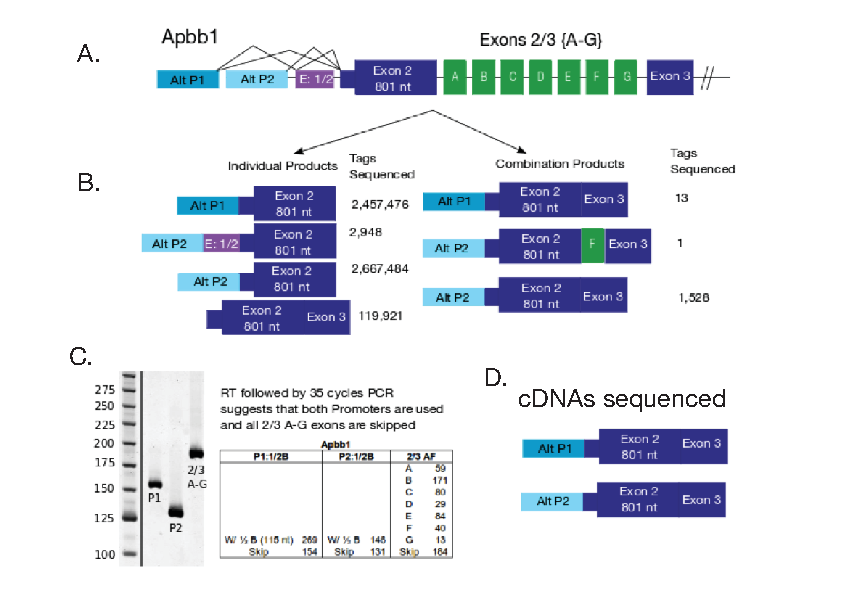
\includegraphics{Figures/SeqZipMethod/Apbb1.eps}
    \caption[Measuring \textit{Apbb1} via SeqZip in multiplex study]
    {
      Measuring \textit{Apbb1} via SeqZip in multiplex study\\[0.25cm]
      A) Region of \textit{Apbb1} investigated. Two alternative promoters, a 5\textprime~cassette exon (``E:1/2'') and a 3\textprime~group of cassette exons (``Exon 2/3 \{A--G\}''). B) Number of sequencing reads mapping to individual \textit{Apbb1} ligation products (left) and combination (right). C) RT-PCR of total RNA taken from a mouse brain looking for cassette exon usage at each position shown in (A). Also shown in the size in nt of the expected bands. D) Schematic of cDNAs cloned and sequencing from mouse brain total RNA.
      }
    \label{SeqZipMethod:fig:Apbb1 Results}
    \end{figure}

\section{RNA Integrity}
  \label{SeqZipMethod:sec:RNA Integrity via SeqZip}

  An exciting use of SeqZip is rapid quantification of RNA integrity. Integrity defined as the faction of molecules that are continuous and unbroken nucleic acid polymers, from the original site of transcript to 3\textprime~processed end. Quantification of integrity has many uses including: (1) quality control of RNA before downstream analysis such as RT or sequencing, and (2) implications of infectivity for viruses that package RNA genomes in virions.

  \subsection{Demonstration of Concept}
    \label{SeqZipMethod:subsec:SeqZip can be used to examine viral genomes}

    In order to demonstrate the feasibility of the SeqZip assay toward performing these type of analysis, I \textit{in vitro} transcribed a 9,800 nt long RNA that I digested using ZnCl$_{2}$ at two different concentrations and times (Figure \ref{SeqZipMethod:fig:Ligation product and RNA integrity}). The RNA was probed using three ligamers, two to the very edges of the RNA and one that looped out the intervening 8,000 nt. The amount of product observed should be directly tied to the abundance of the full length template.

	  \begin{figure} % Degraded RNA measurement by SeqZip
    	\centering 
    	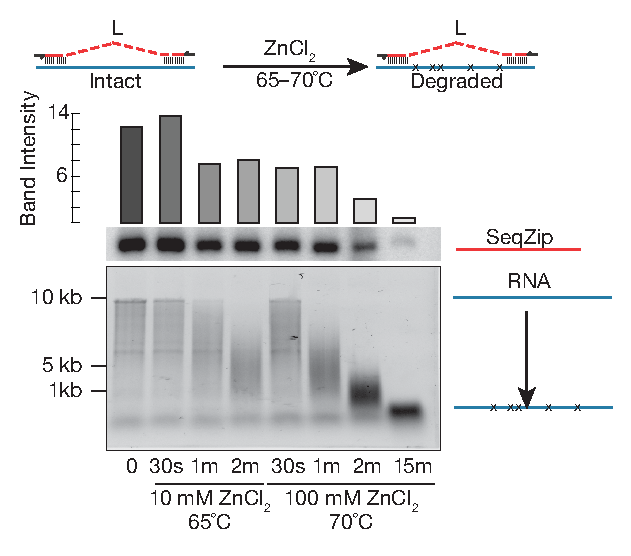
\includegraphics{Figures/SeqZipMethod/DegreadedRNABySeqZip.eps}
    	\caption[Ligation product tied to RNA integrity]
    	{
		    Ligation product tied to RNA integrity\\[0.25cm]
      	Top) Schematic demonstrating SeqZip analysis of transcript integrity. A middle ligamer (L), that hybridizes to the edges of a 8,000 nt section of RNA should only ligate to flanking ligamers when the template RNA is intact. \\
        Middle) Intensity of PCR products amplified using end-labeled primers such that the intensities of all bands can be quantitatively compared (i.e. semi-quantitative PCR). Bottom) A denaturing agarose gel stained with EtBr showing the intactness of the template RNA used in position-matched ligation reactions in the middle panel.
    		}
    	\label{SeqZipMethod:fig:Ligation product and RNA integrity}
  		\end{figure}

    Figure \ref{SeqZipMethod:fig:Ligation product and RNA integrity} shows promising results toward the ability of SeqZip to report on RNA integrity. The apparent intensity of the bands shown in (middle) was tied to the amount of intact RNA seen in (bottom). However, the lane where the RNA was degraded for two minutes with 10 mM ZnCl$_{2}$ compared to 30 seconds with 100 mM ZnCl$_{2}$ were not in good agreement, with clearly less intact RNA in the two minute lane, but just as much ligation product. We hypothesized that this was due to inherent secondary structure in the template we used (a section of the HIV genome, discussed in section \ref{SeqZipMethod:sec:RNA Integrity via SeqZip}). 

    At what concentration of template do ``long'' ligamers generate ligation products from template fragments? We sought to address this question using pools of ligamers targeting either 1) a complete template or 2) \textasciitilde 1 kb 5\textprime~ and 3\textprime~ transcript fragments. The same template used in Figure \ref{SeqZipMethod:fig:Ligation product and RNA integrity} was used for these experiments. SeqZip was performed using a 1:1 ratio of RNA fragments. Results (Figure \ref{SeqZipMethod:fig: trans Tx for degradation}) show that SeqZip accurately reports on the presence of fragments, and not full length transcripts at $\le$1 nM template. This is in good agreement with results presented in Chapter \ref{SeqZipPaper}.

  	\begin{figure} % Trans RNA with SeqZip
    	\centering 
    	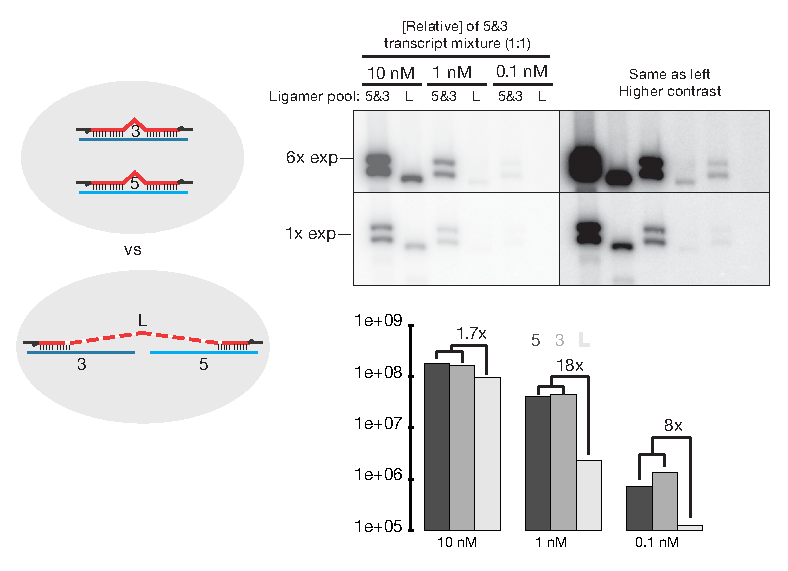
\includegraphics{Figures/SeqZipMethod/TransRNAWithSeqZip.eps}
    	\caption[Trans Transcript investigation]
    	{
	      \textit{Trans}-transcript investigation\\[0.25cm]
  	    Left) Schematic of experimental design: Three pools of ligamers were used. Two (labeled ``3'' and ``5'') hybridize to the 5\textprime~and 3\textprime~sections of a 9,800 nt template RNA. The last, labeled ``L'' connects these two regions via a long longer with target 5\textprime~and 3\textprime~regions of complementarity. (Right;Top) Combinations of the ligamer pools were used with different concentrations of template RNA in the SeqZip assay. Ligation products were amplified with end-labeled PCR primers and amplified using radioactive PCR. Shown are low (left column) and high (right column) versions of two different exposure times (1x on bottom and 6x on top). Right Bottom) Quantification of the bands shown in the gel above, grouped by input template RNA concentration. The fold difference in band intensity between the lowest signal ``5'' or ``3'' ligamer pool and the ``L'' pool is indicated. Y-Axis is the raw band intensity.
		    }
   	 \label{SeqZipMethod:fig: trans Tx for degradation}
	 	 \end{figure}

     These results are encouraging, but bear repeating in order to address the issues of potential secondary structure and repetitive regions inherent to the template RNA used. Put differently---they should be repeated with a traditional mRNA template, instead of a highly-structured and repetitive RNA such as the HIV genome.

  \subsection{HIV Genome Integrity}
    \label{SeqZipMethod:subsec: Why use SeqZip to look at HIV genomes}

    In late 2010--early 2011, a graduate student in the \href{http://profiles.umassmed.edu/profiles/display/133484}{Gottlinger} lab, Anna Kristina Serquiña observed that HIV produced from a cell line expressing ATPase-defective forms of the SF1 helicase UPF1 \citep{Bhattacharya2000} did not infect reporter cell lines the same as control. Previous mass-spec results had reported MOV10 (a SF1 family helicase \citep{Gregersen2014}) was packaged into extracellular viral particles. Anna hypothesized that the decrease in infectivity was due to a problem with RT when the genetic material is introduced into target cells. The results of this study were recently published \citep{Serquina2013}.

    Anna was interested in using SeqZip to quantify intact HIV virus in virus-producing cells and extracellular virions. The first step in applying SeqZip to HIV was to design ligamers.

	\subsection{HIV Ligamer Design}
    \label{SeqZipMethod:subsec: Design of HIV ligamers}

	  Research into the integrity of the HIV RNA genome using SeqZip began with designing a set of ligamers against two different clones. The first, targeting transcripts from the M19921 plasmid (so called ``M'' clone), and the section from the K03455 clone containing nearly identical sequence. We targeted a difference in sequence for one site of ligation (\ref{SeqZipMethod:fig:Hiv tx via SeqZip})A). Three different pools of ligamers were created: a Five(5) ligamer pool, with three ligamers designed to test for the presence of sequence in the first 1,140 nt of the HIV genome, importantly the first site of ligation in the 5 region pool contained a mismatch in the K clone sequence; a three(3) pool, testing the last 1,210 nt of the genome, and a Long (L) ligamer pool, also containing three ligamers, but the middle ligamer of which spans the 5 and 3 regions, looping out 8,633 nt of sequence in the middle of the HIV genome. 

    \textit{In vitro} transcripts were created using both the K and M clones. These transcripts were added to a background of total MEF RNA, and SeqZip was performed. Ligation products were successfully amplified from all ligamer pools when using the M clone transcript and all three ligamer pools. The abundance of these ligation products, as measured by endpoint PCR, seemed to be spike-concentration dependent. Notably, ligation products were not obtained from the K clone using either the 5 or L ligamer pools, likely due to the mismatch between the transcript and the ligamers at the site of ligation. Also of note was the appearance of ligation products from purified endogenous virions of the M clone from all three ligamer pools, and the absence of products from virions purified from plasmids containing a defective protein, Gag, essential for viral packaging. 

	  \begin{figure} % HIV Via SeqZip
  	  \centering 
	    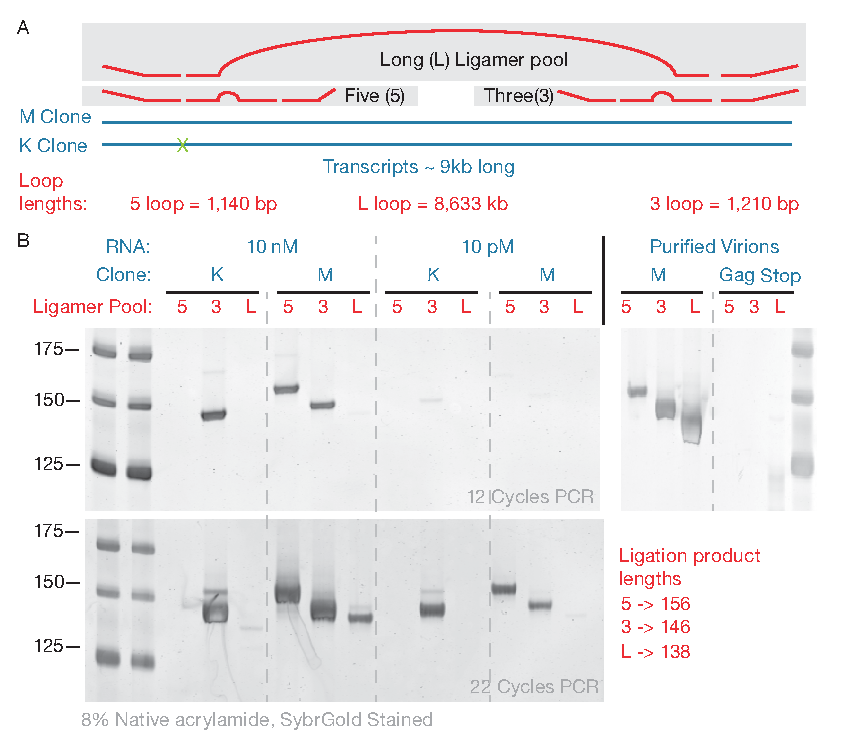
\includegraphics{Figures/SeqZipMethod/HIVviaSeqZip.eps}
    	\caption[SeqZip can examine HIV transcript integrity]
    	{
	      SeqZip can examine HIV transcript integrity\\[0.25cm]
      	A) Schematic demonstrating the experimental design. Three different pools are used to probe for connectivity on the 5\textprime~(Five(5)) and 3\textprime~(Three(3)) ends. Additionally, a Long (L) ligamer is used to check for connectivity between the two ends. We used two different clones of the HIV genome, described in the text and denoted as ``M'' and ``K''. Important here is that the ``K'' contains difference base at a ligation site of the 5 ligamer pool.
        B) A series of end-point PCR gels showing amplified ligation products templated with \textit{in vitro} transcribed RNA at 10 nM or 10 pM of either the K or M clones, or from purified virions of (M clone origin). Show are two different end points of PCR, 12 cycles (top) or 22 cycles (bottom). Also shown is a legend of expected ligation products lengths
    		}
    	\label{SeqZipMethod:fig:Hiv tx via SeqZip}
  		\end{figure}

    The results show (Figure \ref{SeqZipMethod:fig:Hiv tx via SeqZip}) that SeqZip and these three pools of ligamers can be used to profile \textit{in vitro} HIV transcripts and RNA from purified virions. Important features of the figure are: (1) Ligation products are \textit{not} observed for ligation reactions using the K clone template RNA and the Five(5) pool of ligamers, verifying the specificity of the ligamers to the different base of the M clone; and (2) the amount of product from reactions using the L pool of ligamers required more cycles (22 vs 12) in order to be visualized, as would be expected given the physical constraint of hybridizing to two sequences separated by >8,000 nt. 

    Access to purified material and a general push to publish Anna's UPF1 story lead the Gottlinger lab to substantiate the viral genome integrity claims effecting infectivity using a traditional northern blot \citep{Serquina2013}. However, these results are encouraging and warrant additional optimization and application of SeqZip to RNA integrity measurements.

\section{piRNA Precursors}
  \label{SeqZipMethod:sec:Demonstrating continuous precursor TX by SeqZip}

  The first genome-wide studies of piRNAs in \flies{} suggested their production from a long, single-stranded RNA, as discussed in section \ref{Intro:sec:Nucleic Acid Polymers} \citep{Brennecke2007,Gunawardane2007}. Yet, demonstration of precursor transcripts existing as continuous, long, RNA molecules had, as of 2010, yet to be demonstrated. If it could be shown through experimentation that precursors existed as long RNAs, it would provide valuable clues as to their biogenesis, included how such a long RNA is packaged and transported around the cell. With these goals in mind, the following section describes efforts to demonstrating the continuity of precursor transcripts using SeqZip.

  \subsection{Mammalian piRNA Precursor Loci}
    \label{SeqZipMethod:subsec:Mammalian Loci of precursor Tx}

    Chapter \ref{MolCel} discuses 214 genomic loci that account for >95\% of all pachytene piRNAs. Many of these loci are intergenic. That is they reside many thousands of base pairs away from another protein-coding gene. Yet many of these loci \textit{are} traditional protein coding genes themselves, making investigation into their eventual biogenesis to mature piRNAs more complicated. Finally, some loci are generated from what appear to be bidirectional promoters. Figure \ref{SeqZipMethod:fig:precursor Loci Locations} shows the location of each of these types of precursor loci on each of the 19 autosomal chromosomes of the mouse. There were no loci identified on the X and Y chromosomes, likely due to transcription silencing during gametogenesis. 

    \begin{figure} % Precursor Transcript Summary
      \centering 
      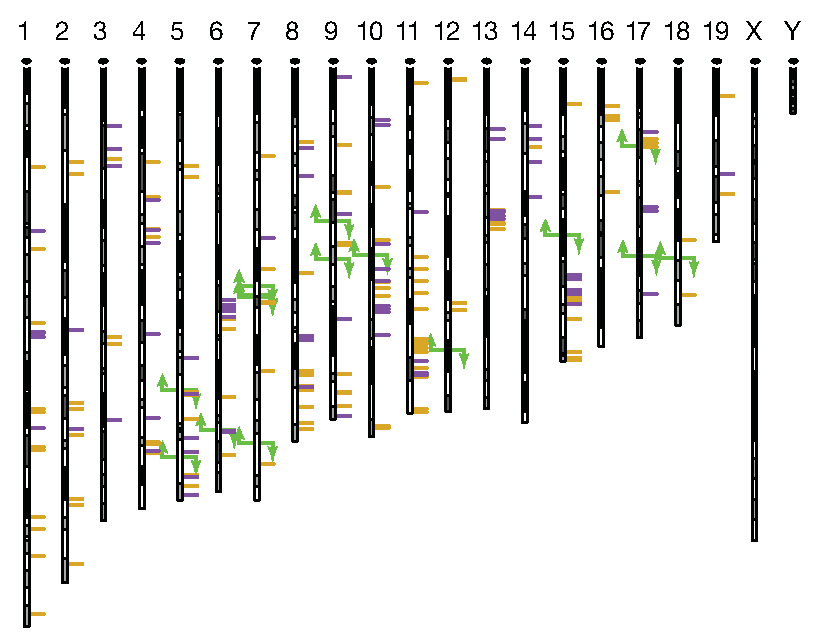
\includegraphics{Figures/SeqZipMethod/PrecursorLocations.eps}
      \caption[Pachytene piRNA precursor locations in mice]
      {
        piRNA precursor locations in mice\\[0.25cm]
        Shown are the 19 autosomal and 2 allosomal mouse chromosomes. They are banded according to ideogram staining and oriented with the centromere (dark black circle) on the top. Yellow bars indicate the location of classified ``pre-pachytene'' loci, which are mostly coincident with previously annotated mRNAs. Purple bars indicate pachytene loci, and are usually far from any other annotated transcript. Finally green arrows, pointing in opposite directions, represent those pachytene loci that are divergently transcribed from a single promoter.
     	 }
      \label{SeqZipMethod:fig:precursor Loci Locations}
      \end{figure}

    The bidirectionally-transcribed sub-type of the pachytene loci are extremely interesting and useful. A motif search of the small sequence between the annotated 5\textprime~TSSs of these transcripts allowed for identification of A-MYB as the transcription factor that drove loci transcription (see section \ref{MolCel:subsec:A-Myb controls Pachytene precursor Tx}). Also, even as the 214 loci account for >95\% of the adult pachytene piRNAs, one could consider just 5 of these promoters, including 4 that drive bidirectional transcription, and account for >50\% of the pachytene piRNAs. Table \ref{SeqZipMethod:tab:matchedClusterValues} describes these loci and transcripts, along with the cumulative number of piRNAs accounted.

    \begin{table} % Top 5 Promoters generate >50% of 14.5 dpp piRNAs
      \caption{Just 9 piRNA genes create >50\% of mammalian piRNAs}
      \label{SeqZipMethod:tab:matchedClusterValues}
      \small
\begin{tabular}{llrrr}
\textbf{Cluster Name} & \textbf{\begin{tabular}[c]{@{}c@{}}Matched \\ Cluster\end{tabular}} & \textbf{\begin{tabular}[c]{@{}c@{}}Unique-mapping \\ piRNAs @ \\ wt.14dpp\end{tabular}} & \textbf{\begin{tabular}[c]{@{}c@{}}Fraction of \\ pachytene \\ piRNAs\end{tabular}} & \textbf{\begin{tabular}[c]{@{}c@{}}Cumulative\\  pachytene\\  piRNAs\end{tabular}} \\ \hline 
17-qA3.3-26735.1      & 17-qA3.3-27363                                                      & 3,021,022                                                                               & 17.2                                                                                & 17.2                                                                               \\        
17-qA3.3-27363.1      & 17-qA3.3-26735                                                      & 1,742,695                                                                               & 9.9                                                                                 & 27.2                                                                               \\        
9-qC-31469.1          & 9-qC-10667                                                          & 1,006,333                                                                               & 5.7                                                                                 & 32.9                                                                               \\        
9-qC-10667.1          & 9-qC-31469                                                          & 272,385                                                                                 & 1.6                                                                                 & 34.5                                                                               \\        
7-qD2-24830.1         & 7-qD2-11976                                                         & 652,564                                                                                 & 3.7                                                                                 & 38.2                                                                               \\        
7-qD2-11976.1         & 7-qD2-24830                                                         & 280,312                                                                                 & 1.6                                                                                 & 39.8                                                                               \\        
6-qF3-28913.1         & 6-qF3-8009                                                          & 564,930                                                                                 & 3.2                                                                                 & 43.0                                                                               \\        
6-qF3-8009.1          & 6-qF3-28913                                                         & 180,210                                                                                 & 1.0                                                                                 & 44.0                                                                               \\        
2-qE1-35981.1         & NA                                                                  & 1121042                                                                                 & 6.4                                                                                 & 50.4                                                                               \\ \hline 
\end{tabular} % Top 5 Promoters generate >50% of 14.5 dpp piRNAs
      \end{table}
    

    Currently, the Zamore lab is designing sequence-specific DNA modifications (via TALENs and CRISPRs) to remove these promoters from the mouse genome. Once strains are created with these promoters removed, it is hoped that the phenotypes displayed will provide clues to the function of pachytene piRNAs in mice.

  \subsection{Pachytene Precursors are Unique Pol II Transcripts}
    \label{SeqZipMethod:subsec:pachytene Tx are different}

    Though mammalian piRNA precursor transcription is driven by Pol II, transcripts themselves have a unique architecture. They tend be very long (some are >100 kb). While not especially long compared to some annotated mRNAs, what is unique is that many are not interrupted by introns for tens of thousands of nucleotides. Given the coupling between splicing and transcription (discussed in section \ref{Intro:subsec:Coordination in splicing}) it is strange to see so much transcribed RNA, surely containing cryptic splice sites, be largely skipped by the spliceosome. Perhaps more confusing is that pre-pachytene precursors \textit{do have} traditional mRNA-like design and introns typical of Pol II transcripts. Yet, both types of transcripts are processed into piRNAs. How does the cell partition these transcripts (see section \ref{Disc:subsec:How are precursors generated})? Also refer to Figure \ref{SeqZipMethod:fig:piRNA precusor Tx features} for comparisons between ``genic'' (i.e. prepachytene) and ``intergenic'' (i.e. pachytene) precursor transcripts (see Appendix \ref{Appendix:tab:GenicAndInterGenicLoci}) and two other classes of Pol II transcripts, mRNAs and non-coding RNAs (ncRNA).

    \begin{figure} % General features of piRNA precursor transcripts
      \centering 
      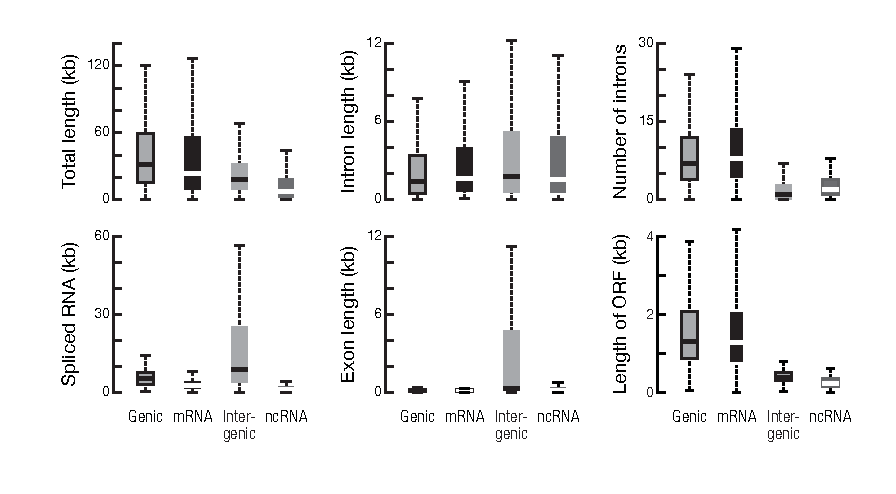
\includegraphics{Figures/SeqZipMethod/piRNAPrecusorTXFeatures.eps}
      \caption[Some general features of piRNA transcripts]
      {
        Some general features of piRNA transcripts\\[0.25cm]
        Top, left) Comparison between genic piRNA precursor transcripts (i.e. pre-pachytene), mRNAs, Intergenic precursor transcripts (i.e. pachytene), and non-coding RNAs (ncRNA) for overall length in nucleotides. Top, middle) Intron length. Top, right) Number of introns. Bottom) Same as above, but considering fully processed (i.e. ``spliced'') versions of the transcripts.
        }
      \label{SeqZipMethod:fig:piRNA precusor Tx features}
      \end{figure}

    An initial goal of characterizing piRNA precursor transcripts was to demonstrate their existence as continuous RNA polymers in total RNA obtained from mouse testes.  Given the tremendous length of these transcripts (Figure \ref{SeqZipMethod:fig:piRNA precusor Tx features}), the go-to experimental approach one would use to demonstrate continuity would be gene-specific RT-PCR. A DNA oligo was designed to hybridize near the 3\textprime~end of the loci \textit{17-qA3.3-27363.1} (\textit{aka} ``M1''), the longest and most studied of the mice piRNA-generating loci. RT would be primed using this oligo, generating cDNAs that would extend (1) until the 5\textprime~end of the transcript was reached or (2) RT fell off the template. Following cDNA generation, pairs of DNA primers hybridizing to 5\textprime~sections of the proposed transcript were used in PCR reactions. Boundaries of the proposed transcript were determined using a combination of small RNA sequencing and poly(A)+-unstranded RNA-Seq. A schematic of the approach is shown in Figure \ref{SeqZipMethod:fig:RT doesn't work for precursors}A.

    One expected issue when performing RT on such a long transcript expressed at low levels is the \textit{lack} of dependence on the RT primer. This is illustrated in Figure \ref{SeqZipMethod:fig:RT doesn't work for precursors}B, where in the ``+RT; -Primer'' lanes there is still a clear signal for all 7 primer pairs. The signal is virtually gone when leaving out RT, suggesting that an RNA template is the source of the signal. It is believed that extremely short DNA species (as short as 4 nt) are priming the RT at some very low rate in the ``-Primer'' reactions. This complication removes RT-PCR as a suitable experimental approach to demonstrate the continuity of piRNA precursor transcripts.

    \begin{figure} % RT doesn't work for piRNA precursor Transcripts
      \centering 
      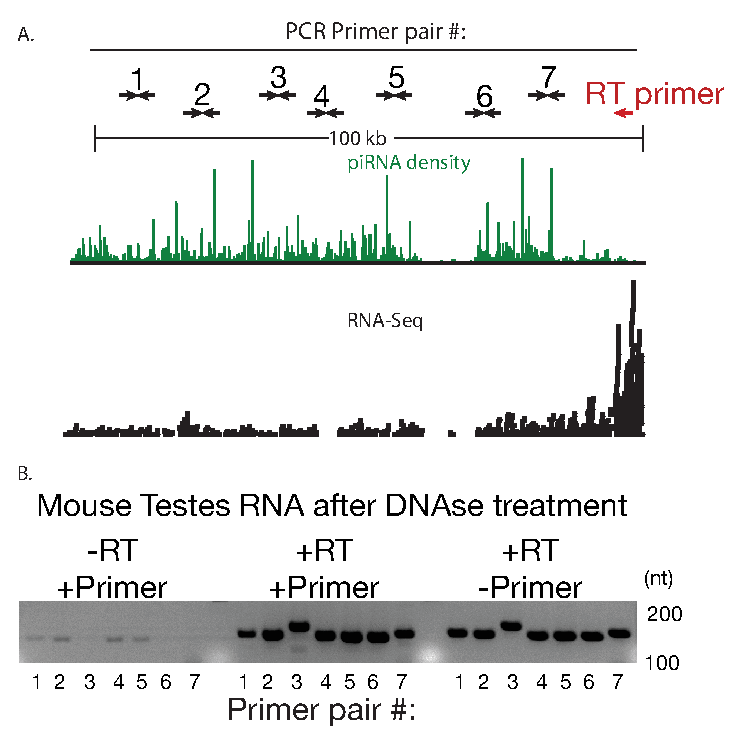
\includegraphics{Figures/SeqZipMethod/RTDoesntWork.eps}
      \caption[pRT Doesn't Work for piRNA precursors]
      {
        RT Doesn't Work for piRNA precursors\\[0.25cm]
        A) Experimental design of RT-PCR demonstration of piRNA precursor \textit{17-qA3.3-27363.1} continuity. Shown in black, numbered 1-7 are primer pairs amplified by PCR, after cDNA generation using the red ``RT primer''. Also shown is the length of the locus, the small RNA signal in green, and the RNA-Seq signal in black. The locus is shown 5\textprime~(left) to 3\textprime~(right). B) Results from RT-PCR using the 7 primer pairs shown in A, and various combinations of $\pm$ RT-primer and RT-PCR enzyme.
      	}
      \label{SeqZipMethod:fig:RT doesn't work for precursors}
    	\end{figure}

  \subsection{Connectivity of Distance Intramolecular Sequences}
    \label{SeqZipMethod:subsec:SeqZip on long RNAs at multiple locations}

    Before applying SeqZip to these extremely difficult transcripts, we designed a set of oligos to demonstrate the continuity of a traditional mRNA. The mRNA picked, \dst{}, was (1) of sufficient length (>23 kb as a fully processed mRNA) and (2) expressed in mouse testes. Ligamers were designed to loop out \textasciitilde5kb sections spaced evenly along the length of the transcript. A ligamer was designed to loop out 22 kb of the message, from 5\textprime~to 3\textprime~end. An illustration of the experimental design is shown in Figure \ref{SeqZipMethod:fig:SeqZip on dst1}.

    \begin{figure} % SeqZip does work for Dst1 transcripts
      \centering 
      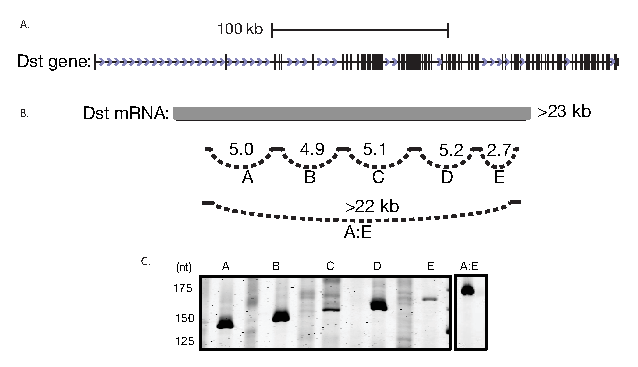
\includegraphics{Figures/SeqZipMethod/dst1.eps}
      \caption[SeqZip on a very long mRNA (\dst{})]
      {
        SeqZip on a very long mRNA (\dst{})\\[0.25cm]
        A) A model of the \dst{} gene. Arrows show direction of transcription (5\textprime~to 3\textprime~). Exons are tall lines, intronic regions join the exons. A scale bar is shown for size in kb. B) A schematic showing how SeqZip was used to investigate 5 different regions of \dst{} transcripts (called A-E). Indicated are the nt of each loop in kb. C) End-point PCR of SeqZip ligation products from each of the ligamer sets shown in (B). 
        Unmarked lanes show failed A:B; A:B:C; A:B:C:D; and A:B:C:D:E multi-loop combinations. For the ligations that did work, looping ligamers were ligated to non-looping ``control'' ligamers immediately adjacent, in order to show that just a three-ligation reaction could work. Reaction A:E used a single ligamer to span all the RNA of the individual loops and was ligamer to adjacently-hybridized ligamers.
        }
      \label{SeqZipMethod:fig:SeqZip on dst1}
      \end{figure}
        
    As seen in Figure \ref{SeqZipMethod:fig:SeqZip on dst1}C, ligation products were obtained from every ligamer combination, including the critical set (``AE'') where >22 kb of the message was looped out. In the control experiment, no ligation products were observed. This experiment represents the longest successful ``looping'' in a SeqZip experiment targeting an endogenously expressed RNA.

    An additional demonstration of SeqZip's application to profile long RNAs at multiple sites are experiments involving \fn{}. As described previously (see section \ref{SeqZipPaper:subsec: Method Development and Validation}) \fn{} contains three main sites of alternative splicing: EDB, EDA, and the V-region. Using the proper mix of ligamers, SeqZip examines and maintains connectivity at all three of these sites, correctly reporting on their usage in the RNA template (Figure \ref{SeqZipMethod:fig:Three Site FN1 by SeqZip}). With these results in hand, we felt confident that SeqZip could be used to analyze piRNA precursor transcripts.

    \begin{figure} % Investigating Three sites of FN1 using SeqZip
            \centering 
            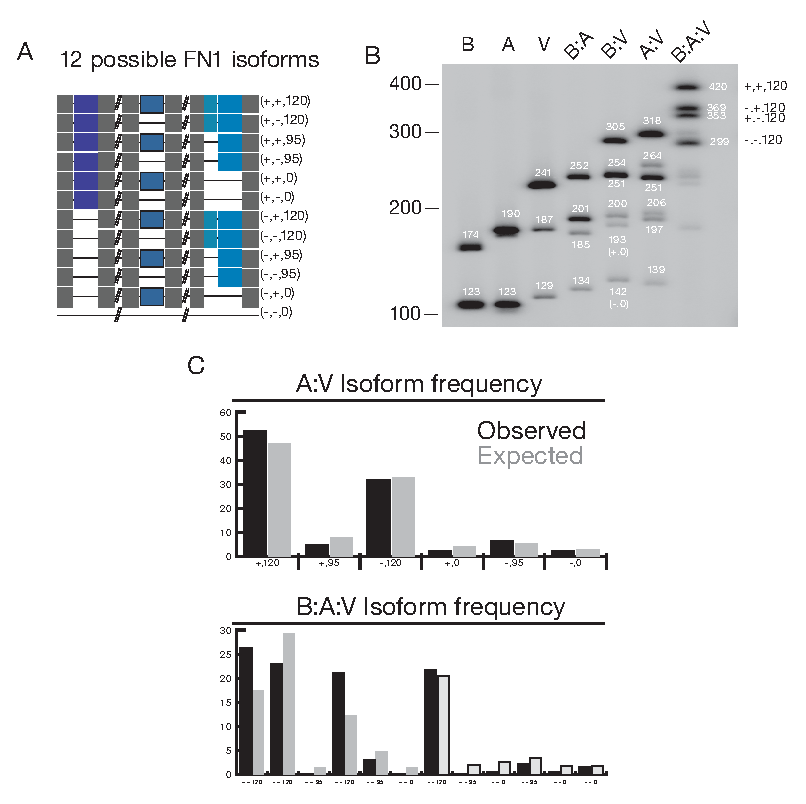
\includegraphics{Figures/SeqZipMethod/fn1ThreeSite.eps}
            \caption[Three sites of alternative splicing in \fn{} by SeqZip]
            {
              Three sites of alternative splicing in \fn{} by SeqZip\\[0.25cm]
              A) Graphical representation of the 12 possible isoforms from mouse \fn{}. B) Radioactive PCR gel showing amplified ligation products templated with specific loops of ligamers. Pools are specified by top row: B = EDB exon only; A = EDA exon only; V = V-Region only; B:A = EDB and EDA exon combinations; B:V = EDB and V-Region combinations; A:V = EDA and V-Region combinations; B:A:V = All two combinations, as shown in panel (A). Marked in nt is shown on left, expected size of specific ligation ligation products indicated in white letters on the gel, or black on right side. Where identity is not obvious from size, identity of isoform provided. C) Quantification of bands from panel (B). Black bars = observed signal of indicated band, Grey = product of individual frequencies. Top only describes A:V combinations, lower shows all combinations.
              }
            \label{SeqZipMethod:fig:Three Site FN1 by SeqZip}
            \end{figure}

  \subsection{Precursor Transcript Continuity}
    \label{SeqZipMethod:sec:piRNA precursor by SeqZip}

    Applying the same logic as that used to examine multiple distant sequences in \dst{} and \fn{}, ligamers were designed against a highly-expressed piRNA-producing loci, \textit{7-qD2-11976} (aka - ``M11''). Five unique sites were picked, again named A-E. Sites were picked to (1) avoid repetitive regions; (2) overlap with expression evidence from small RNA and RNA-Seq data; (3) contain loops of \textasciitilde5 kb in length; and 4) be unique in the genome. A schematic of the approach is shown in Figure \ref{SeqZipMethod:fig:Precursors are testes-specific}A.

    Using total RNA obtained from adult mouse testes, analyzed by SeqZip and the ligamers shown in Figure \ref{SeqZipMethod:fig:Precursors are testes-specific}A, signal from ligation products could routinely be observed from loops of \textasciitilde5 kb (Figure \ref{SeqZipMethod:fig:Precursors are testes-specific}B-left and Figure \ref{SeqZipMethod:fig:M1 analysis by SeqZip}B). Also the signal is dependent on source RNA (Figure \ref{SeqZipMethod:fig:Precursors are testes-specific}B-right) and RNA from HEK293 (Human Embryonic Kidney) cells did not produce ligation products. The M1 and M11 clusters are both long and have reasonably high expression compared to the other precursors. Yet, no ligation products were ever obtained for either cluster when loops >\textasciitilde5 kb were used (data not shown). What was the cause of this negative signal?

    \begin{figure} % Precursors Transcripts are Testes Specific
        \centering 
        \includegraphics{Figures/SeqZipMethod/testesSpecificRnaseqPrecursors.eps}
        \caption[piRNA precursor Ligation products from Mouse Testes RNA and not HEK293 Cell RNA]
        {
          piRNA precursor Ligation products from Mouse Testes RNA and not HEK293 Cell RNA\\[0.25cm]
          A) Schematic of the piRNA-producing loci (``gene'') \textit{7-qD2-11976} (aka ``M11'') shown with scale bar, and relative looping ligamer locations.  Loops are labeled A-E, and the length of the loop in kb is shown.  Also shown in green is small RNA expression along this locus. B Left) Ligation products obtained from each set shown in (A) using mouse testes RNA, or B Right) HEK293-cell RNA was used to test for ligation products resulting from non-specific RNA. Similar to Figure \ref{SeqZipMethod:fig:SeqZip on dst1}, unmarked lanes contain failed A:B; A:B:C; A:B:C:D; and A:B:C:D:E multi-loop combinations.
        	}
        \label{SeqZipMethod:fig:Precursors are testes-specific}
      	\end{figure}

    \begin{figure} % M1 precusor analysis by SeqZip
        \centering 
        \includegraphics{Figures/SeqZipMethod/piRNAPrecurserAnalyisBySeqZip.eps}
        \caption[SeqZip signal from piRNA-producing loci \textit{17-qA3.3-27363.1}]
        {
          SeqZip signal from piRNA-producing loci \textit{17-qA3.3-27363.1}\\[0.25cm]
          A) Schematic of the piRNA-producing loci \textit{17-qA3.3-27363.1} (aka ``M1'') shown with scale bar, and relative looping ligamer locations.  Loops are labeled A--G and the length of the loop in kb.  Green is small RNA expression along this locus and RNA-Seq in black. B) Ligation products obtained from each set shown in (A) using mouse testes RNA.
        	}
        \label{SeqZipMethod:fig:M1 analysis by SeqZip}
      	\end{figure}
          
    As first alluded to in Chapter \ref{SeqZipPaper} and discussed in section \ref{SeqZipMethod:sec:Multiplex Gene Study}, ligation efficiency should decrease with loop length and additional required ligations. All of the ligation products used to profile precursors only required two ligation events. Numerous other genes had been investigated with SeqZip that contained >2 sites of ligation (sections \ref{SeqZipPaper:sec:Discussion} and \ref{SeqZipMethod:subsec:SeqZip on long RNAs at multiple locations}). This suggested that the length of the loops was the limiting factor in obtaining ligation products templated off piRNA precursors.

    We investigated this potential explanation by designing a series of ligamer sets with increasing 1 kb increment loop lengths from 5--10 kb. Figure \ref{SeqZipMethod:fig:piRNA precusors and loop length} shows results typical of this series of experiments. The amount of ligation product when using ligamers of increasing loop size decreases with the length of the loop. The signal, after 35 cycles of end-point PCR, is barely visible when the loop is 9 kb, and extremely faint when 10 kb. Ten kilo-bases represents just a fraction of the length of some pachytene piRNA precursor transcripts. 

    \begin{figure} % SeqZip precusor signal decreases with loop length
      \centering
      \includegraphics{Figures/SeqZipMethod/piRNAprecusorM1SignalDecreasesWithLoopLength.eps}
      \caption[SeqZip signal from piRNA precursor transcripts decreases with loop length]
      {
        SeqZip signal from piRNA precursor transcripts decreases with loop length\\[0.25cm]
        A series of ligamers were design against the 5\textprime~portion of cluster \textit{17-qA3.3-27363.1} (``M1''). Sets forcing increasing lengths were used, and ligation products were analyzed by end-point PCR.
        }
      \label{SeqZipMethod:fig:piRNA precusors and loop length}
      \end{figure}

    Even after numerous attempts, ligation products could not be obtained for loop sizes >10 kb, no matter what the target transcript. At this point in the study, we decided to abandon the demonstration of piRNA precursor transcripts as continuous transcripts via SeqZip, and instead turned our attention to splicing within the transcripts (discussed in the next section, \ref{SeqZipMethod:sec:piRNA precursors are spliced}) which eventually lead to the study presented in Chapter \ref{SeqZipPaper}.

    What could be the cause of our inability to create ligation products? The method worked so well, without any optimization, for mRNAs of similar length and expression (e.g. \dst{}). Our current hypothesis is that at steady-state levels, the amount of full-length piRNA precursors that exist---in continuous polymers of length >10kb---is extremely low. Low to the point of being below the SeqZip limit of detection. Indeed, many nucleases appear to act on piRNA precursors along their journey from Pol II transcript to mature piRNA (see section \ref{Intro:subsec:Processing of piRNAs in mice}). The piRNA machinery is perhaps too fast and efficient for us to capture these extremely long RNAs. Future experiments that somehow perturb the pathway, such as \textit{Pld6} (aka \textit{MmZuc, MitoPLD} and \textit{Zucchini} in flies) could accumulate precursors before cleavage occurs.

\section{Precursor Splicing}
  \label{SeqZipMethod:sec:piRNA precursors are spliced}

  Once it was determined that the existence of piRNA precursor transcripts as continuous piRNA precursors could not be demonstrated using SeqZip, careful attention was paid to RNA-Seq data used to determine the edges of precursor loci transcription. The RNA-Seq data, once aligned with a splicing-sensitive algorithm (i.e. ``Tophat'' \citep{Trapnell2009}), showed that piRNA precursors were spliced. Multiple reads and species supported intronic segments and each contained little to no RNA-Seq and small RNA reads. A good example of the high-level type of data observation that was being performed until this point is shown in Figure \ref{SeqZipMethod:fig:evidence for precusor splicing}. In this figure, small RNA data is shown in green along with RNA-Seq data in black. For this particular cluster, the RNA-Seq data and small RNA data appear continuous with the length of gene, as typical for many loci in \flies{}. It was necessary to increase the resolution used to study the piRNA-generating loci in mice in order to accurately define transcripts.

  \begin{figure} % evidence for precursor splicing
    \centering 
    \includegraphics{Figures/SeqZipMethod/evidenceForPrecursorSplicing.eps}
    \caption[Example small RNA and RNA-Seq data aligned to a piRNA-generating loci]
    {
      Example small RNA and RNA-Seq data aligned to a piRNA-generating loci (\textit{17-qA3.3-26735})\\[0.25cm]
      Shown in the context of the genome and surrounding genes (blue) is a piRNA-generating loci, with signal in green. Bottom) zoomed view of the small RNA signal (green) along with poly(A)+-unstranded RNA-Seq (black).
      }
    \label{SeqZipMethod:fig:evidence for precusor splicing}
    \end{figure}

  One of the most illustrative piRNA-generating loci is that containing the genes \textit{17-qA3.3-27363.1 and 17-qA3.3-26735} (Figure \ref{SeqZipMethod:fig:no piRNAs within Precursor Introns}). These two genes are expressed in pre-pachytene testes and increase expression once mice hit 14.5 dpp. These two genes alone account for 27\% of all the piRNAs sequenced at 14.5 dpp (see Chapter \ref{MolCel} and Table \ref{SeqZipMethod:tab:matchedClusterValues}). A extremely informative feature, detected early from initial poly(A)+-unstranded RNA-Seq libraries, was the absence of signal near the apparent 3\textprime~end of the loci. There were many reads that could be aligned across this gap, as if it was a traditional mRNA intron. There were no repeat element that would have depleted this region of the message for reads, as with other sections of the locus. The most obvious explanation was that the precursor contained an intron, which was spliced out prior to poly(A) tailing.

  \begin{figure} % No piRNAs in introns
    \centering 
    \includegraphics{Figures/SeqZipMethod/noPiRNAswithinPrecusorIntrons.eps}
    \caption[Introns in mammalian piRNA precursors]
    {
      Introns in mammalian piRNA precursors\\[0.25cm]
      Top) Divergently transcribed piRNA-producing genes \textit{17-qA3.3-27363.1 and 17-qA3.3-26735}. These genes are transcribed from a common promoter. Plus strand small RNAs are shown in blue, minus stranded small RNAs in red. poly(A)+-unstranded) RNA-Seq is shown in black. Bottom) Zoomed portion of the message near the 3\textprime~end of \textit{17-qA3.3-26735}. Plus-stranded small RNA (blue) and RNA-Seq reads in black. Multiple RNA reads and species aligned across a intron. This region was also largely free of small RNA signal.
      }
    \label{SeqZipMethod:fig:no piRNAs within Precursor Introns}
    \end{figure}

  The results shown in Figure \ref{SeqZipMethod:fig:no piRNAs within Precursor Introns} were very exciting initially, and provided important clues to the biogenesis of piRNAs. The presence of an intron indicates Pol II origin. The lack of small RNA within the intron supported mature piRNA creation after precursor splicing. A major reason why this feature had not already been noticed is that small RNA data is not long enough to accurately and confidently align across splice junctions. Therefore, intron detection had to wait for application of longer RNA-Seq reads and splicing-sensitive alignment software. Once these introns were known, supporting their use with small RNA data become possible.

  Using genomic coordinates supplied by the splicing-sensitive alignment algorithm \citep{Trapnell2009}, an alignment index of transcript sequences \textit{flanking} the introns was created. Then, using a more traditional (in terms of small RNA alignment) aligner, Bowtie \citep{Langmead2009}, those piRNAs that did \textit{not} map to the genome could be aligned to index containg piRNA precursor splice junctions. This experiment is shown graphically in Figure \ref{SeqZipMethod:fig: piRNAs map to SJ}.

  \begin{figure} % piRNAs map to splice junctions
    \centering 
    \includegraphics{Figures/SeqZipMethod/smallRNAsMapToPrecursorSJ.eps}
    \caption[piRNAs map to precursor transcript splice junctions]
    {
      piRNAs map to precursor transcript splice junctions\\[0.25cm]
      Top) piRNA density (green) and RNA-Seq density at the 3\textprime~most intron within \textit{17-qA3.3-26735}. Bottom) A splice junction sequence (blue) created by joining the sequences just outside the intron shown in (Top) is sufficient to align non-genome mapping piRNAs.
      }
    \label{SeqZipMethod:fig: piRNAs map to SJ}
    \end{figure}

  Chapter \ref{MolCel} discusses the ultimate refinement of the observations described above, including the generality of splicing within precursor transcripts. In fact, there are a total of 383 introns within the ``intergenic'' sub-classified 214 piRNA-generating loci from \citep{Li2013e} (see Table \ref{Appendix:tab:GenicAndInterGenicLoci}). These introns display a A-MYB\textendash dependent small RNA signal across their exon-exon junctions (Figure \ref{SeqZipMethod:fig: amyb makes SJ mapping}). The more traditionally looking piRNA-producing loci of the ``genic'' subclass, contain far more introns (2,113). The signal for these transcripts does not display the same A-MYB\textendash dependent small RNA signal.

  \begin{figure} % A-Myb mutants do not have SJ-mapping piRNAs
    \centering 
    \includegraphics{Figures/SeqZipMethod/aggregatePiRNAsatSpliceJunctions.eps}
    \caption[\amyb{} Mutants produce no splice-junction mapping piRNAs for genic piRNA-producing loci]
    {
      \amyb{} Mutants produce no splice-junction mapping piRNAs for genic piRNA-producing loci\\[0.25cm]
      Trimmed mean ppm of junction-mapping piRNAs within two classes (``genic \& Intergenic'') loci. Shown in red is signal from \amyb{} mutant mice, black \amyb{} heterozygous mice. All data from stranded RNA-Seq (strand accounted for during alignment and signal aggregation).
      }
    \label{SeqZipMethod:fig: amyb makes SJ mapping}
    \end{figure}

  While it was not possible to demonstrate continuity of piRNA-producing precursors using SeqZip, development of advanced HTS methods and computational approaches provides clear evidence that they are (see Chapter \ref{MolCel}). Proposed future experiments into mammalian piRNA precursors are discussed in section \ref{Disc:sec:piRNA precursors}.

\cleardoublepage
  % !TEX root = /Users/royc/Google_Drive/Thesis/RoyC_Umass_Thesis.tex
\chapter{Discussion} \label{Disc}
\lhead{Chapter 5. \emph{Discussion}} 
%----------------------------------------------------------------------------------------

\section{The Future of Dynamic long RNAs}\label{Disc:sec:Future of Dynamic long RNAs}

  Deep sequencing of transcriptomes has revolutionized biology. Previously, transcript discovery was a cumbersome task. Transcript identification and characterization involved significant labor, cost, and materials. In the mid-90's, microarray technology \citep{Schena1995a} gave us a tantalizing glimpse into how genes were expressed, but were limited to probed, and therefore known, sequences. Yet, the green and red landscapes of a microarray analysis hinted at incredible complexity \textemdash a complexity that would have to wait for technology to catch up.

  Like many transformative technologies, RNA-seq was made possible by incremental improvements to numerous supportive technologies such as: 1) digital optics; 2) microscopy; 3) slide chemistry and on-slide PCR; and 4) nucleic-acid alignment. A HiSeq 2500 relies on all of these technologies (and others) to produce the 100M+ sequences that allow scientists to peer every day into the transcriptional output of a genome.

  In the past 5 years, biologists have started to think way beyond mRNAs and small RNAs. The former captured out interest for 30+ years \citep{Furuichi1975,Wei1975}, and the later has been on a run-away train since capturing out attention in 1998 \citep{Fire1998}. HTS has added long RNAs to these classes of gene products. However, many biologically-trained and minded Scientists find themselves overwhelmed by the complete different methods and approaches to tackling the ``big data'' created by modern genome-wide experiments. Experimental training does not currently provide students with the required skills in statistics, computer programing, and experimental design that are needed to work with genome-wide data (see section \ref{subsec: Biologists need Comp Skills}. The richness of this data often leaves many unasked (and unanswered) test-able hypothesis just sitting in public repositories \citep{Plocik2013}.

  At this point, it is important to remember that in this document \textit{long RNAs} may also refer to products containing characteristics of traditional mRNAs, that is a 5\textprime~m7G Cap, ligated exons, and a Poly(A) tail. However, many of these long mRNAs are extremely dynamic. So much so that until HTS and RNA-Seq, comprehensive investigation of their complexity was not possible.

  \subsection{Pervasive transcription}\label{Disc:subsec:Pervasive Tx}

    The encode project revealed that most of the genome is transcribed into RNA. This was done in cancerous cell lines, and while it revealed the potential for transcription, it did not reveal much biology beyond cells in culture simply perpetuating their existence. 

    
    The ENCODE papers from late 2012 suggested that 95\% of the genome is functional \citep{Dunham2012}, a finding that continues to be heavily debated \citep{Graur2013,Bhattacharjee2014}. \citet{Djebali2012} and focused on issues of transcription in these cell lines, as discussed in section \ref{sec:IsoformsPerGene}. The ENCODE studies were performed an human cancerous cell lines from different sources, and they still saw tremendous transcriptional diversity. With better HTS tools and resolution, we should fully expect ever increasing estimates of transcriptome diversity once accurate catalogues and assemblies from tissues, cells, and single single cells are possible.

    Additionally, GENCODE version 7 includes 9,640 manually curated lncRNA loci \citep{Derrien2012}. 
    % Insert additional thoughts from the Tomari Review in EMBO Reports.

  \subsection{Accurate and complete transcript annotation}\label{Disc:subsec:Accurate and complete Tx annotation}

    A deck of cards has only 52 cards, but can delt into $2,598,960$ different 5 cards hands, as when playing Poker. There are $1,098,240$ different single-pair combinations, with a probability of obtaining one being almost 50\%. Compare this to ``Royal Flush'', for which there are only 4 options, and a probability of $649,739:1$ or $1.54 * 10^{-6}$ !. It is these numbers that makes possible to play Poker for hours on end. Long ago, biologic evolved to arrange genes into unique and rare combinations, especially in eukaryotic organisms. Indeed the process of splicing is closely correlated with organism complexity. The process of AS is even more closely tied to organism complexity (see figure \ref{Disc:fig:numGenesAndNumSpliced}).

    Accurate determination and assembly of each card (exon) that comprises a hand (transcript) is a major known unknown of research into long RNA. The current state of the field is described in section \ref{subsec: Tx Assembly}. This field is in its infancy. Each gain in resolution or sensitivity reveals more complexity. Yet transcript assembly algorithms only provide predictions and probabilities for the existence of real molecules. Until RNA can be directly sequenced, in their entirety, from single cells, researchers will always be making compromises for transcript annotation and quantification. Once technology advances to the point where a transcriptome can be as accurately and quickly determined as a genome, extremely exiting research into the more subtle and nuanced complexity (e.g. what makes one twin molecularly different from another?) of biology can be unlocked.

    \todo[inline]{What is required to better transcript annotation?} % **************************

  \subsection{Tissue and cell specificity}\label{Disc:subsec:Tissue-specific Tx expression}

    \todo[inline]{Discuss feelings of tissue-specific RNA expression} % **************************
    % Include ideas from Brown2014 that states that AS is actually tissue-specific splicing.

\section{Lingering Questions for \dscam{}}\label{Disc:sec:Dscam}

  What controls the stochastic and probabilistic splicing of \dscam{}? Why is it different between hemocytes and neurons? Why would hemocytes need less apparent diversity, given the range of antigen they could potentially encounter?

  Can methods such as RNACapture be used to perform more careful and targeted sequencing of \dscam{} transcripts \citep{Mercer2014}?

  \todo[inline]{Mention RNACapture \citep{Mercer2014}} % **************************

\section{In the haystack: piRNA precursor transcripts surrounded by RNA}\label{Disc:sec:piRNA precursors}


  Chapter \ref{MolCel} describes efforts to annotate 467 transcripts from 214 loci that account for 95\% of the total piRNAs in 14.5 dpp mice. Also described is how these transcripts are typical Pol II transcripts, possessing all the archetypical molecular signatures including 5\textprime~MeGppp caps, introns, and poly(A) tails. Yet RNA from these molecules appears to be rapidly consumed and processed into millions of unique 24\textendash32 nt species. How does the cell partition long RNAs for translation by the ribosome (as the case for most mRNAs) or cleavage and maturation into piRNAs? The sections below propose experiments aimed toward answering this question.

  \subsection{How are they generated?}\label{Disc:subsec:How are precursors generated}

    % From the resources paper: Indeed, two isoforms of pi-Wdfy3 are transcribed from different promoters in the testis (Figure S2D). The short isoform is transcribed from a low CpG promoter bound by A-MYB, while the long isoform is transcribed from a high CpG with no detectable A-MYB binding. piRNAs derive from the genomic region corresponding to the short transcript. In an A-Myb mutant, piRNA from the pi-Wdfy3 loci are reduced 165-fold (31.6 rpkm in heterozygotes versus 0.191 in mutants). The abundance of long isoform transcripts did not decrease (2.08 rpkm in heterozygotes versus 3.86 rpkm in mutant), while the small isoforms became undetectable (10.0 rpkm versus 0 rpkm), consistent with the idea that the short, but not the long, Wdfy3 transcript is a piRNA precursor RNA. Little is known about the regulation of genic piRNAs, because only seven genic piRNA loci are A-MYB-dependent (Li, et al., accompanying manuscript). We do not yet know if such differential regulation of transcript isoforms occurs more generally for genic piRNA loci.

    %How does cell partition prepachytene transcripts to mRNA or piRNA use?
    What determines that a seemingly mRNA-like piRNA precursor is processed into piRNAs, and not translated like crazy by Ribosomes?  Everything meets the ribosome ($REF$), so why is it that precursors are given a different lot in life?

    \begin{figure} % pi-Wdfy3 expresses both mRNA and piRNA precursor transcript
      \centering 
      \includegraphics{Figures/Discussion/pi-wdfy3.eps}
      \caption[\wdfy{} locus expresses both mRNA and piRNA precusor form in testes]
      {\wdfy{} locus expresses both mRNA and piRNA precusor form in testes\\[0.25cm]
        The mouse genomic locus \wdfy{} expresses both a traditional mRNA form, originating from an upstream TSS, and a piRNA precursor transcript from a downstream TSS. The piRNA precursor form appears to originate from an A-MYB-bound promoter, and is expressed in \amyb{} heterzygous mice. Also smalll RNAs (piRNAs) mapping to this locus are only observed in \amyb{} heterzygous mice, and not in \amyb{} mutant mice.
        }
      \label{Disc:fig:wdfy3}
      \end{figure}

    %Interaction w/ ribosomes?

  \subsection{What are they doing?}\label{Disc:subsec:What are piRNAs doing}

    \todo[inline]{What are piRNAs doing in Mammals?} % **************************

  \subsection{In vivo chemical labeling of precursor piRNA transcripts}\label{Disc:subsec:Labeling of precursors}

    % From Resources Paper: Despite sharing many features with protein-coding genes, intergenic piRNA loci stand out as a unique class of transcriptional units. Almost half contain no introns

    % Need section here on the chemical modification - what were you thinking? Azide? Par-Clip?  Maybe a CLASH-like assay?  What about what Mihir is developing?
    
    SeqZip accurately reports on the presence of multiple, distant sequences contained in the same RNA molecule (see Chapters \ref{Chapter2} and \ref{Chapter3}). Yet I was not able to observe ligation products templated off some of the most highly-expressed precursor transcripts (see section \ref{sec: precursor TX}. We hypothesize that the most likely explanation for being unable to observe ligation products for these transcripts, but successfully observing those for a very long, but lowly expressed gene   extit{Dst}, suggests that precursor transcripts are rapidly processed into mature piRNAs. What if this is not the case if we could hybridize ligamers to precursor transcripts in vivo? Put another way  extemdash What if the steady-state amount of precursor transcript is very low due to rapid processing, but when visualized in real time, the transcripts are of sufficient abundance for FISH? Ligamers could be engineered to contain different combinations of fluorescent dyes, and the proximity and intensity of the signal could be used to infer precursor transcripts. Importantly, this approach could distinguish long, continuous precursor transcripts from processing intermediates and mature piRNAs.

  \subsection{In vivo imaging of precursor piRNA transcripts}\label{Disc:subsec:Imaging of precursors}

    %Another idea would be to image the precursors in real time somehow. How about tagging them and following them in the sperm? That could be cool. You could even follow them into the developing embryo. 
    The most important question for mammalian \textit{pachytene} piRNAs is \textit{What are they doing?}. We know that they are essential for the health of the species, as discussed in section \ref{c3-intro}, and piRNA-pathway mutants are sterile. What could these small RNAs, with complementarity to nothing but themselves, be doing? Building on the last section discussing chemical modification precursor transcripts, if the modification was again durable enough for downstream analysis, perhaps the modification would remain in the mature piRNAs that are incorporated into mature sperm. These modifications could be tracked as the sperm move through the \hl{semineferous tubues} and into the $SPERM ANATOMY$. One could even track the piRNAs as they fuse with the oocyte to create an embryo. If this modification was labile, piRNA interacting proteins or nucleic acids could be captured or marked as well, providing additional clues as to the function of piRNAs in sperm and early embryogenesis.

    The cellular location of precursor piRNA transcript processing is not known. The most accepted hypothesis is that precursor transcripts are processed into mature piRNAs with machinery tethered to chromatoid bodies \citep{Meikar2014} or another structure similar to Drosophila Nuage ($REF$) near the mitochondrial cement ($REF$). Knowledge of \textit{where} mature piRNAs are generated would provide clues into larger mechanist details of their biogenesis. 

    I can think of two broadly different ways in which we could pinpoint the physical location of mature piRNA generation. The first is to chemically label, in some manner, primary piRNA transcripts. The label would need to 1) not interfere with processing and 2) be durable to later methods used to analyze the presence or absence of the modification. A second way to identify the location of mature piRNA processing would be to actually observe, through in vivo \hyperref[hd:abrevs]{FISH}, the various products and by-products of biogenesis. In this particular approach, SeqZip maybe useful.

    % MS2 lopp introduction into piRNA precursor transcripts.
    Another idea here would be to use the MCP x MBS mouse as published by the Singer lab \citep{Park2014}. In this paper they insert multiple MS2 binding loops into the 3  extprime~-UTR of the $beta$-actin gene, and cross it with another mouse that has MCP (MS2 Bacteriophage capsid protein) fused to GFP. Using this system they can visualize   \textit{endogenous} mRNAs in cultured MEF cells, and brain sections. How could we apply this to imaging of piRNA precursor transcripts? If we inserted an MS2 loop into the tail end of transcripts, what would we see? It is certainly worth it!

  \subsection{FISSEQ of piRNA precursor transcripts}

    \todo[inline]{Write FISSEQ application to piRNA precursor Tx} % **************************

    % When researchers measure gene expression, they typically read the aggregate RNA abundance over a population of cells. But just as not all stadium-goers cheer when the home team scores during a baseball game, single cells don’t necessarily behave the same as the population as a whole. As a result, researchers increasingly are turning to single-cell methods.

    % Single-cell transcriptome sequencing (RNA-seq) is one option, but it loses subcellular localization information by effectively treating the cell as a homogenous sphere. Another choice, RNA fluorescent in situ hybridization (FISH), maintains subcellular detail but supports exploration of only four or five transcripts at once.

    %Now George Church, Professor of Genetics at Harvard Medical School, and colleagues have developed a technique they call FISSEQ (fluorescent in situ RNA sequencing), which blends the power of RNA FISH and RNA-seq to report the subcellular localization of several thousand genes simultaneously (1).

    %The new RNA-focused method relies on rolling circle amplification to create a three-dimensional grid of “DNA nanoballs,” each representing a single RNA molecule locked in its original subcellular location. SOLiD ligation-based sequencing then reads 27 to 30 bases from each nanoball, and the fluorescent output is read in three dimensions via confocal microscopy.

    %The method identified several thousand transcripts per experiment (4171 in one experiment, 8102 in a second), showing relatively good concordance with both RNA-seq and DNA microarray datasets for moderately expressed genes. Low and high abundance genes correlated less well, but the former are less reliably quantitated in all methods, Church noted, whereas the latter are mostly protein- and RNA-processing transcripts, which typically are bound up in nucleoprotein complexes. “Probably the only ribosomal RNAs we detect haven’t been packaged into ribosomes,” he speculated. Importantly, FISSEQ not only picked up expected transcripts, but also matched their expected subcellular localizations.

    %Mats Nilsson, Professor of Biochemistry and Biophysics at Stockholm University, who in 2013 described a similar in situ transcriptomic approach (2), noted that Church’s method is unbiased, whereas Nilsson’s used molecular inversion (padlock) probes to amplify specific transcripts.

    %“I really think this is an important step towards more contextual sequencing, bringing next-generation sequencing into the spatial domain,” he said.

    %Church’s group is applying FISSEQ to studies of mouse and human brains, where the method can be applied to classify cells and, if paired with barcoding, even map cellular connectivity. “We see this as one of the key enabling technologies for the BRAIN initiative,” said Church.
    %References
    %[1] J.H. Lee et al., “Highly multiplexed subcellular RNA sequencing in situ,” Science, 343:1360–3, Feb. 27, 2014.
    %[2] R. Ke et al., “In situ sequencing for RNA analysis in preserved tissue and cells,” Nat Meth, 10:857–60, 2013.

\section{Future uses of SeqZip}\label{Disc:sec:Future Uses of SeqZip}

  SeqZip can be used to many different forms of RNA sequence characterization. An incomplete illustration of these applications is shown in Figure \ref{Disc:fig: Panel of SeqZip Applications}. The three novel applications are discussed below:

  \begin{figure} % SeqZip uses Panel
    \centering 
    \includegraphics{Figures/Discussion/SeqZipUses.eps}
    \caption[Proposed uses of the SeqZip methodology]
    {Proposed uses of the SeqZip methodology \\[0.25cm]
      Shown here are general applications of the SeqZip method to profiling RNA sequences. Top row examples are substantiated by experiements described on Chapters \ref{SeqZipPaper} and \ref{SeqZipMethod}, the middle and lower rows are hypothetical but logical extensions of the method.
      }
    \label{Disc:fig: Panel of SeqZip Applications}
    \end{figure}

  \subsection{Multi-site SNP detection}\label{Disc:subsec: Multi-site SNP Detection}

    \todo[inline]{Mention Which side to put the Mismatch} % **************************
    % Cite the newest Shuman paper, and the Shuman crystal papers

  \subsection{Introduction of destruction sequences}\label{Disc:subsec:Intro of Desctruction Sequences}

    \todo[inline]{Discuss Type III restriction enzymes, etc} % **************************

  \subsection{Multi-site FISH probes}\label{Disc:subsec:Multi-site FISH probes}

    % What about applying the Church lab's new technique of in situ sequencing? Would this help us differentiate transcripts from mature piRNAs?  

\section{SeqZip Assay Improvements}\label{Disc:sec:SeqZip Improvements}

  The SeqZip methodology as developed and described in Chapters \ref{SeqZipPaper} and \ref{SeqZipMethod} works adequately and robustly for characterization of relatively simple (\cd{}) to extremely complex (\dscam{}) genes. However, there is still substantial room for method optimization. Two obvious areas of improvement include the reduction of ligation time and NTL product formation. The improvements and modifications discussed below should assist in achieving these two (among other) goals.

  \subsection{LNA-containing ligamers and T39A Rnl2}\label{Disc:subsec:LNA-Containing ligamers and T39A Rnk2}

    The use of an RNA-base on the 5\textprime~ side of the nick encourages a C3\textprime~\textit{endo} sugar pucker for the base, placing the 3\textprime~OH in an apical orientation relative to the the AMP leaving group (see Figure \ref{Disc:fig:Rnl2 and suger pucker}) \citep{Nandakumar2006}.

    \begin{figure} % Rnl2 Suger Pucker
      \centering 
      \includegraphics{Figures/Discussion/Rnl2_and_suger_pucker.eps}
      \caption[Suger pucker in Rnl2 structures]
      {Suger pucker in Rnl2 structures \\[0.25cm]
        Using two different nucleic acid substrate combinations crystallized with Rnl2, \citet{Nandakumar2006} demonstrates the effect of 3\textprime~ and 2\textprime~ identify of the base at the 5\textprime~ side of the nick: Left) The crystal structure (PDB: 2HVS), containing a 2\textprime~ position deoxy residue, displays a DNA-like C2\textprime~\textit{endo} sugar pucker. In contrast to Right) where the crystal structure (2HVR) contains a 2\textprime~ hydroxyl and displays an RNA-like C3\textprime~\textit{endo} sugar pucker.
        }
        \label{Disc:fig:Rnl2 and suger pucker}
        \end{figure}

    With lowered costs of oligo synthesis, incorporation of 2\textprime~OMe at the penultimate and ultimate bases of the 5\textprime~ nick ligamers should greatly increase ligaiton efficiency, as these are the primary substrate-specificity determinants of Rnl2 \citep{Nandakumar2004a, Nandakumar2006}.

    Interestingly, \citet{Nandakumar2004a} demonstrated that the ribosome at the penultimate position, evidenced by a 50-fold reduction in turnover number for 2\textprime~H substitutions at this position, compared to full activity for 2\textprime~OMe. \citet{Nandakumar2006} (see Figure \ref{Disc:fig:Rnl2 and suger pucker} shows that Threonine 39 (T39) hydrogen bonds with both the 2\textprime~OMe and 3\textprime~O of the penultimate suger. A T39A mutation did not phenocopy the 2\textprime~H substitution on the penultimate suger, indicating that suger pucker is the structural constraint on ligation efficiency. These results indicate that a T39A mutant of Rnl2 may demonstrate increased RNA-templated DNA:DNA ligation efficiency, as it would have one less molecular requirement for RNA.

    Future versions of the SeqZip assay could use a combination of LNA modified bases \citep{You2006} at either the penultimate or terminal residues on the 5\textprime~side of the nick in order to increase 1) specificity, and 2) enzyme efficiency. The combination of these modifications in the ligamers could be combined with a T39A mutant form of Rnl2 for a potentially greatly enhanced ligation rate.

  \subsubsection{Thermostable Ligases}\label{Disc:subsec:Thermostable Ligases}

    The use of LNA-containing brings up issues involving off-target hybridization. Future iterations of the SeqZip methodology could use directed protein evolution of Rnl2 \citep{Stemmer1994, Romero2009a} to develop a thermostable variant of Rnl2, similar to variations of DNA ligase that have been used for years \citep{Barany1991}. Use of LNAs and elevated ligation temperatures could alviate off-target hybridization events reducing both nonproductive hybridization and non-templated ligation events. This would also allow for use of reduced overall ligamer concentrations, in line with the optimal SeqZip experiment described in section \ref{subsec: Ideal multiplex study} and synthesis on microarrays.

  \subsection{Re-purposing the SOLiD Platform}\label{Disc:subsec:SOLiD Platform for SeqZip}

    \todo[inline]{SOLiD Application of SeqZip} % **************************

    The ability to incorporate custom sequuences into ligations, which subsequently are incorporated into ligation products provides tremendous opportunities for downstream analysis (see figure \ref{Disc:fig: Panel of SeqZip Applications}).

  \subsection{Quantifying ligation and PCR events}\label{Disc:subsec:SeqZip and QPCR}

    Digital PCR of the PCR products ala \citep{Shiroguchi2012a}. 

  \subsection{Reducing required input RNA and ligamer concentration}\label{Disc:subsec:Reducing Input RNA and Ligamer Conc.}

    SeqZip on single-cell RNA samples.

  \subsection{An ideal SeqZip experiment to query coordinated splicing}\label{Disc:subsec: Ideal SeqZip exp. to look for Coordination}
    \label{Disc:subsec: Ideal multiplex study}

    If I could go back in time 4 years and still possess the knowledge and abilities that I do now, I would have approached a genome-wide study of coordination in splicing using SeqZip much differently. First, I would have focused on alternative first exon (or promoter, or TSS) and potential coordination with downstream cassette exons. I would have mined newly-generated RNA-Seq data \citep{Wang2008, Pan2008} for alternative first exons and cassette exons of sufficient expression. Then, I would have used my automated ligamer design software (see Appendix \ref{Appendix:AutoMatedLigamerAssembly}), to create a database of the required ligamers. As this would require at least 3 ligamers per event, with very little duplicated use of ligamers, the number of ligamers would make standard synthesis, even using 384-well plates, impossible. Therefore, I would have pursued printing the ligamers on a custom microarray, and cleaved them into solution, similar to products offered by \href{http://www.nimblegen.com/}{Nimblogen}. These ligamers would be barcoded and priming sequences included such that short (50nt) paired-end reads could reliably identify the templated first and cassette exons. Using this pool of ligamers, I would have performed the SeqZip assay, including a barcoding scheme to quantify the number of ligation events per {alt first exon::cassette exon} pair. Also, the libraries would have been amplified via digital PCR allowing me to check for PCR jackpots \citep{Shiroguchi2012a}. Finally, the data would be aligned against a reference of all \{alt first exon::cassette exon\} pairs, and any potential coordination determined.

    If I could have done the experiment designed above, I feel the full potential and utility of the SeqZip method could have been realized and generated new and valuable knowledge for the field of gene expression.

  \subsection{SeqZip and single-molecule FISH}\label{Disc:subsec:SeqZip and Single-Molecule FISH}

    \begin{figure} % Multi-site Fish using SeqZip
      \centering 
      \includegraphics{Figures/Discussion/MultiSiteFish.eps}
      \caption[Multi-Site smFISH using flourophore-containg ligamers]
      {Multi-Site smFISH using flourophore-containg ligamers \\[0.25cm]
        \hl{Insert Caption Here}
        }
      \label{Disc:fig:MultiSite FISH using SeqZip}
      \end{figure}

\section{Final thoughts}\label{Disc:sec:Final Thoughts}

  \subsection{Biologists need Computation Biological Skills}\label{Disc:subsec:Biologists need Comp Skills}

    Just 10 years ago,  Graduate students and PhDs in the fields of Molecular Biology or Biochemistry need not venture far from data analysis within Excel or perhaps a statistical program with an advanced graphical interface (examples include Prism or Graphpad). Software knowledge that stops at these tools and the rest of the Microsoft Office suite of tools is no longer enough to generate big strides in Biomedical research.

    Working with tens of even hundreds of lines of data within a spreadsheet is manageable and computers from 20 years ago had more then enough computing power to process the data. Yet, this type of data is longer then endpoint of most cutting edge projects. Many students and post docs often find that they are unable to analyze the data generated from months or years of tireless bench work. Faced with learning what is effectively a collection of new languages and awash in a sea of acronyms (LINUX, BASH, GNU, PERL, R) they reach out for help from a ``Bioinformatics person.'' Perhaps the relationship and interaction with this personal is productive, leading to a collaboration and exciting new knowledge. Sometimes it isn't, and the bench scientist shifts into one of three modes: 1) Wait; 2) Find another bioinformati1c-minded collaborator; or 3) collect more data.

    In my experience, the most often chosen mode is ``wait.'' This is also the most damaging, as it delays the progress of one's work, and the advancement of science in general. Personally, I did not want to fall into this mode, and once the multiplex study described in section \ref{sec: Multiplex Gene Study} reached a point where I had millions of sequencing reads, but I could not find anyone to help me analyze the data, that I decided to educate myself on the basic principles of Linux, the command line, and analysis of HTS data.

    A Biologically-train individual who posses the knowledge of analysis of HTS datasets is an extremely powerful and empowering situation. This was recently commucated in \citet{Plocik2013}:

    \begin{quote} % Polick2013 Quote about insight without a Pipette
      \itshape 
      Such exercises will empower students to explore and assess the quantitative data published in the manuscripts that they read, which can no longer be assessed at a glance like the qualitative gel-based results on which molecular biology was founded. Ultimately, it will be equally important to know how to write code as it is to pipette. - \citep{Plocik2013}
      \singlespacing
      \end{quote}

    The fact is that no one will care about a project as much as the Graduate student or PostDoc who is the main project driver. Learning and training of computational skills bent on analyzing large datasets should be central to the education in Biomedical sciences in the future.

  \subsection{Science versus Engineering: Two thoughts in one school}\label{Disc:subsec:Science and Engineering}

    \begin{quote}
      \itshape 
      \singlespacing
        “There is a general attitude among the scientific community that science is superior to engineering.” - \citep{Macilwain2010}

      “Science is about what is; engineering is about what can be. Engineers are dedicated to solving problems and creating new, useful, and efficient things.“ - Niel Armstrong
      \end{quote}

    A common schism between technically-oriented individuals is whether or not they identify themselves as an engineer or a scientist. The first quote, from an article published in Nature, communicates a clear bias in academic circles of the importance of the   extit{why} over the   extit{how}. In essence, how one priorities these questions may categories individuals as a scientists (why is important) or an engineer (how is more important). The second quote, from the first man to walk on the Moon, Neil Armstrong, highlights what motivates a self described ”engineer” and ”geek.” How does a single graduate system, training PhDs for careers in life science, educate individuals who fall into these two fundamentally different belief systems?
    In short  extemdash not well. When searching for a lab to call home, I told professors that I wanted to work on a technology development project. A typical response was, “That's not what we do here.” As someone who is first interested in the ``how'' over the ``why,'' this began a brief period when I thought I had made the wrong choice in leaving industry to go back to graduate school. What was the basis for this aversion to technology development? The same article in Nature states that this feeling toward engineering may be attributed:

    \begin{quote} 
      \itshape 
      \singlespacing
      ...partly to a ``linear'' model of innovation, which holds that scientific discovery leads to technology, which in turn leads to human betterment.  This model is as firmly entrenched in policy-makers' minds as it is intellectually discredited.  As any engineer will tell you, innovations, such as aviation and the steam engine, commonly precede scientific understanding of how things work.
      \end{quote} 

    If policy-makers value basic discovery over technological application, perhaps this explains why many of my professors tried to steer me away from a technology development project.

    In spite of policy-makers and my professors holding the viewpoint that discovery precedes technology, some of the most notable breakthrough scientific discoveries, including many made by Nobel Laureates, demonstrate a clear integration of both the scientific method and technological application.  For example, the 2007 award in Physiology and Medicine was given for “discoveries of principles for introducing specific gene modifications in mice by the use of embryonic stem cells."  By combining these principle discoveries, an indispensable technique in modern genetics was created – gene targeting.  The feeling of which is more important, the principle discoveries or the application thereof, is likely what separates a scientist from an engineer. 

    The importance of technology to the advancement of science in general is not limited to anecdotes resulting in a Nobel prize. A quick scan of the most \href{http://www.pnas.org/reports/most-cited}{highly-cited} papers in the journal PNAS reveals that the top 13, indeed   extit{all} 13, are about a novel methodology or technique. Sequencing of DNA, microarray analysis, tetracycline-ineducable promoters, recombinant adenovirus, and site-specific mutagenesis are just a handful of the tools on this list. This effect can be seen in \href{http://simplystatistics.org/2014/04/07/writing-good-software-can-have-more-impact-than-publishing-in-high-impact-journals-for-genomic-statisticians/}{computation biology}, with transformative techniques, such as BLAT \citep{Altschul1990} and Bowtie \citep{Langmead2009} attaining citations well beyond a typical paper in their journal of publication and far more than most primary research-centered articles.

    How does someone who is motivated by the engineering of science best contribute in an academic setting? Luckily, I did not have to question my decision to return to school for long. I found a pair of labs where I could learn how to practice traditional hypothesis-driven research while also developing new tools necessary to do so. My project is a perfect fit for me and has been terrific fun to work on. In the past five years, the technique that I developed, SeqZip, allows for the more efficient study of  mRNA isoforms produced from alternative splicing of pre-mRNA. This is a very engineering-type accomplishment. However, the technique uses short DNA oligonucleotides and a novel activity (that I discovered) of an known RNA ligase to shorten and simplify isoform sequence information. Use of Rnl2 to perform RNA-templated DNA:DNA ligation is completely new knowledge, and falls squarely within a scientific purview. The technique simplifies many of the experimental issues that researchers struggle with when studying the often complex products of alternative splicing.
    
    \todo[inline]{Need transition or concluding paragraph} % **************************
    
  \subsection{Dealing with the data deluge}\label{Disc:subsec:Dealing with Data Deluge}

    \todo[inline]{Writing about HTS data management}

    How do we work with all this data? Mention LabKey, GenomeBridge, Define the scope of the problem, etc...

    I would love to have a database of complete transcripts of a cell - think about how you were panning the data for the MolCel paper, and you could see ChIP marks, Pol II occupancy, RNA-Seq, and piRNA data. It would be great to be able to do that more often, and we greater precision
 
  \appendix % Cue to tell LaTeX that the following 'chapters' are Appendices
  \label{hd:Appendicies}
  \setstretch{1} % Line spacing of 1
  % !TEX root = /Users/royc/Google_Drive/Thesis/RoyC_Umass_Thesis.tex
\chapter{Appendix - Misc Information} \label{AppendixMisc:Appendix: Misc Info} 
\lhead{Appendix A. \emph{Appendix: Misc Information}} 


\section{Buffers}\label{AppendixMisc:sec:Buffers}

  \renewcommand{\arraystretch}{1}
    \begin{table}[ht]
    \centering
      \begin{tabular}[c]{c|c}
      Component & Concentration \\
        \hline
      Tris-HCl  & 50 mM         \\
        \hline
      MgCl2     & 2 mM          \\
        \hline
      DTT       & 1 mM          \\
        \hline
      ATP       & 400 $\mu$M        \\
        \hline
      pH        & 7.5 @ 25\degree~C   
      \end{tabular}
    \caption[SeqZip Hybridization and Ligation Buffer]
      {
      SeqZip Hybridization and Ligation Buffer
      }
    \label{AppendixMisc:tbl: Rnl2 Buffer}
    \end{table}

\section{Equations}\label{AppendixMisc:sec: Equations}

\subsection{Determining [RNA] from $^{32}$P-$\alpha$-UTP used during vitro transcription}

{
  \tiny{
    \begin{eqnarray*}
    \mu \mbox{M} = \left( \frac{\mbox{pmol}}{\mu\mbox{L}}\right)
          = \left( \frac{\mbox{cpm after purification} \times \mbox{dilution factor}}{\mbox{cpm before purification} \times \mbox{dilution factor}} \right)
          \times \left( \frac{\mbox{mol UTP in original reaction}}{\mbox{Reaction Volume }} \right) \times \left( \frac{1}{\mbox{Number UTPs in transcript}} \right) \times 10^{-12} 
    \end{eqnarray*}
  }
}
%Or you can write the above equation as 

%\begin{eqnarray*}
%\mu \mbox{M}  =  \left( \frac{\mbox{pmol}}{\mu\mbox{L}}\right)
%     & = & \left( \frac{\mbox{cpm after purification} \times \mbox{dilution factor}}{\mbox{cpm before purification} \times \mbox{dilution factor}} \right)\\
%      && \times \left( \frac{\mbox{mol UTP in original reaction}}{\mbox{Reaction Volume}} \right)\\
%      && \times \left( \frac{1}{\mbox{Number UTPs in transcript}} \right) \times 10^{-12} 
%\end{eqnarray*}


\subsection{Determining [RNA] based on A$_{260}$}

  $$
  \mbox{[RNA in M]} = \left( \frac{\mbox{A}_{260} \times \mbox{Dilution Factor}}
                             {10,313 < \mbox{note 1}> \times \mbox{ nucleotides in message}} \right) 
  $$
  
  note 1: This value represents an average RNA extinction ($\epsilon$) coefficient value \\

\subsection{Normalize oxidized small RNA libraries size to time-matched unoxidized library}

NB: this equation assumes calibration against a specific time-point ,
in this case data obtained from 6 week-old testes.

  \begin{eqnarray*}
    \mbox{unox }\tau \mbox{ norm}_1 & = & \left(         
                          \frac{\left( \frac{\displaystyle\sum \mbox{miRNA reads } \tau}{\displaystyle \sum \mbox{miRNA reads 6wk} } \right) \times \mbox{ depth 6wk} }{1,000,000}              
                                            \right)\\
    \mbox{ox }\tau \mbox{ norm}_1 & = &   \mbox{unox }\tau \mbox{ norm}_1 \times
                                   \left(
                                    \frac{\displaystyle \sum \mbox{oxidized shared } \ge \mbox{23 nt reads}}{\displaystyle \sum \mbox{unoxidized shared } \ge \mbox{23 nt reads}}
                                   \right)                                         
    \end{eqnarray*}

\section{PCR Programs}\label{AppendixMisc:sec:PCR Programs}

\textbf{Ligamer Hybridization}
ROY-H2 | Ligamer Hybridization\\
  Steps 1–9 are 10 minute incubations at the following temperatures:\\
  69;66;63;58;54;52;50;48;46\degree~C\\
  Step 10 is a 45\degree~C incubation for 1 hour\\
  Steps 11–14 are 10 minute incubations at the following templates:\\
  43;41;39;37\degree~C\\
  Final incubation is at 37\degree~C for $\infty$\\

\textbf{SeqZip ligation program}
ROY-37-4 | T4 Rnl2 RNA-template DNA:DNA ligation\\
  1. 37\degree~C for 18 hours\\
  2. 10\degree~C for $\infty$ \\


  \chapter{Appendix B: Automated Ligamer Assembly}\label{Appendix:AutoMatedLigamerAssembly} 
\lhead{Appendix B. \emph{Perl Script for Automated Ligamer Assembly}} 

\section{Installation}

Major Steps:
\begin{itemize}
	\item  Create an input csv file with required information
	\item  Run this information sequentially through the scripts
	\item  Use the results to order oligos from IDT
\end{itemize}

Required Tools:
\begin{itemize}
	\item  Perl
	\item  BioPerl
	\item  Ensembl Perl APIs
	\item  String::Random Perl Package
\end{itemize}

Items to future improvements
\begin{itemize}
	\item Use Ensembl Database to initilize queries
	\item Make the use of BioPerl more flexible
	\item Make more web-friedly
\end{itemize}

Helpful hints on installing BioPerl and Emsembl Perl APIs:

\lstset{language=BASH}
\begin{lstlisting}
	## Install BioPerl, use git
	    cpan App::cpanminus # First prep cpan
	    cpanm DBI ## Install necessary DBI perl module
	    mkdir ~/src; cd ~/src
	    git clone git://github.com/bioperl/bioperl-live.git
	    cp ~/.bash_profile ~/.bash_profile.bak
	    echo -e 'PERL5LIB=$HOME/src/bioperl-live:$PERL5LIB' >> ~/.bash_profile
	    source ~/.bash_profile
	# Install ensembl perl apis
	    mkdir ~/src; cd ~/src
	    wget ftp://ftp.ensembl.org/pub/ensembl-api.tar.gz
	    tar xvfz ensembl-api.tar.gz
	# Add locations to perlfile libs to $PATH
	    echo -e '
	    PERL5LIB=${PERL5LIB}:${HOME}/src/ensembl/modules
	    PERL5LIB=${PERL5LIB}:${HOME}/src/ensembl-compara/modules
	    PERL5LIB=${PERL5LIB}:${HOME}/src/ensembl-variation/modules
	    PERL5LIB=${PERL5LIB}:${HOME}/src/ensembl-functgenomics/modules
	    export PERL5LIB' >> ~/.bash_profile
\end{lstlisting}
%----------------------------------------------------------------------------------------
\section{Example Input Format}
%----------------------------------------------------------------------------------------
\begin{landscape}
Here is an example input file to create ligamers investigating the \textit{Gria3} gene in Rats:
\begin{table}[h]\footnotesize
\begin{tabular}{lcccccccc}
\# Comment lines are ignored\\
\#Gene name\\
~GRIA3\\
\# PCR primers used - Solexa PE adaptor sequences\\
\# Five prime\\
PCR-Primer-5'-ATCTGAGCGGGCTGGCAAGGC\\
\#Three Prime\\
PCR-Primer-3'-GCCTCCCTCGCGCCATCAGA\\
\end{tabular}
\end{table}

\begin{table}[h]\footnotesize
\begin{tabular}{lcccccccc}
ExonId                                                                          & LigID & Name    & Strand & Code & TargetPrime & bedLoc & SetID & ConstID \\
<Gria3\_201/202-Shared-I14                                                        & 10        & rn4 & minus  & TC                   & 5                       & X:127903250-127903350 & NANNNNNN        & 201\_2\_intron    \\
<Gria33\_201/202-Shared-I14                                                        & 9         & rn4 & minus  & T                    & 3                       & X:127903210-127903249 & NNNNNNNN        & 201\_2\_intron    \\
<Gria33\_201/202-E15                                                               & 8         & rn4 & minus  & TC                   & 5                       & X:127914822-127915069 & NNNNNNN         & 201,202           \\
<Gria33\_202-I14:15                                                                & 7         & rn4 & minus  & I                    & N                       & X:127912345-127914821 & TACACAT         & 202               \\
<Gria33\_202-E14                                                                   & 6         & rn4 & minus  & I                    & N                       & X:127912230-127912344 & ACCCCAG         & 202               \\
<Gria33\_201-I14:15                                                                & 5         & rn4 & minus  & I                    & N                       & X:127897499-127914821 & CGCGCAC         & 201               \\
<Gria33\_201-E14                                                                   & 4         & rn4 & minus  & I                    & N                       & X:127897384-127897498 & GTCTCAA         & 201               \\
<Gria33\_202-I13:14                                                                & 3         & rn4 & minus  & I                    & N                       & X:127896828-127912229 & ACCGATT         & 202               \\
<Gria33\_201-I13:14                                                                & 2         & rn4 & minus  & I                    & N                       & X:127896828-127897383 & CGCTATG         & 201               \\
<Gria33\_201/202-E13                                                               & 1         & rn4 & minus  & T                    & 3                       & X:127896580-127896827 & NNNNNNN         & 201,202          
\end{tabular}
\end{table}
\end{landscape}
%----------------------------------------------------------------------------------------
\section{Ligamer Assembler Source Code}\label{apx: Ligamer Assmembler}
%----------------------------------------------------------------------------------------

\lstinputlisting[language=PERL]{Appendices/ligamerAssembler.pl}


  %\chapter{Automated Ligamer Assembly}\label{AppendixC} 
\lhead{Appendix C. \emph{Perl Script for Automated Ligamer Assembly}} 

\section{Installation}

Major Steps:
\begin{itemize}
	\item  Create an input csv file with required information
	\item  Run this information sequentially through the scripts
	\item  Use the results to order oligos from IDT
\end{itemize}

Required Tools:
\begin{itemize}
	\item  Perl
	\item  BioPerl
	\item  Ensembl Perl APIs
	\item  String::Random Perl Package
\end{itemize}

Items to future improvements
\begin{itemize}
	\item Use Ensembl Database to initilize queries
	\item Make the use of BioPerl more flexible
	\item Make more web-friedly
\end{itemize}

Helpful hints on installing BioPerl and Emsembl Perl APIs:

\lstset{language=BASH}
\begin{lstlisting}
	## Install BioPerl, use git
	    cpan App::cpanminus # First prep cpan
	    cpanm DBI ## Install necessary DBI perl module
	    mkdir ~/src; cd ~/src
	    git clone git://github.com/bioperl/bioperl-live.git
	    cp ~/.bash_profile ~/.bash_profile.bak
	    echo -e 'PERL5LIB=$HOME/src/bioperl-live:$PERL5LIB' >> ~/.bash_profile
	    source ~/.bash_profile
	# Install ensembl perl apis
	    mkdir ~/src; cd ~/src
	    wget ftp://ftp.ensembl.org/pub/ensembl-api.tar.gz
	    tar xvfz ensembl-api.tar.gz
	# Add locations to perlfile libs to $PATH
	    echo -e '
	    PERL5LIB=${PERL5LIB}:${HOME}/src/ensembl/modules
	    PERL5LIB=${PERL5LIB}:${HOME}/src/ensembl-compara/modules
	    PERL5LIB=${PERL5LIB}:${HOME}/src/ensembl-variation/modules
	    PERL5LIB=${PERL5LIB}:${HOME}/src/ensembl-functgenomics/modules
	    export PERL5LIB' >> ~/.bash_profile
\end{lstlisting}


%----------------------------------------------------------------------------------------
\section{Example Input Format}
%----------------------------------------------------------------------------------------

%\newgeometry{margin=1cm} % modify this if you need even more space
\begin{landscape}
Here is an example input file to create ligamers investigating the \textit{Gria3} gene in Rats:
\begin{table}[h]\footnotesize
\begin{tabular}{lcccccccc}
\# Comment lines are ignored\\
\#Gene name\\
~GRIA3\\
\# PCR primers used - Solexa PE adaptor sequences\\
\# Five prime\\
PCR-Primer-5'-ATCTGAGCGGGCTGGCAAGGC\\
\#Three Prime\\
PCR-Primer-3'-GCCTCCCTCGCGCCATCAGA\\
\end{tabular}
\end{table}

\begin{table}[h]\footnotesize
\begin{tabular}{lcccccccc}
ExonId                                                                          & LigID & Name    & Strand & Code & TargetPrime & bedLoc & SetID & ConstID \\
<Gria3\_201/202-Shared-I14                                                        & 10        & rn4 & minus  & TC                   & 5                       & X:127903250-127903350 & NANNNNNN        & 201\_2\_intron    \\
<Gria33\_201/202-Shared-I14                                                        & 9         & rn4 & minus  & T                    & 3                       & X:127903210-127903249 & NNNNNNNN        & 201\_2\_intron    \\
<Gria33\_201/202-E15                                                               & 8         & rn4 & minus  & TC                   & 5                       & X:127914822-127915069 & NNNNNNN         & 201,202           \\
<Gria33\_202-I14:15                                                                & 7         & rn4 & minus  & I                    & N                       & X:127912345-127914821 & TACACAT         & 202               \\
<Gria33\_202-E14                                                                   & 6         & rn4 & minus  & I                    & N                       & X:127912230-127912344 & ACCCCAG         & 202               \\
<Gria33\_201-I14:15                                                                & 5         & rn4 & minus  & I                    & N                       & X:127897499-127914821 & CGCGCAC         & 201               \\
<Gria33\_201-E14                                                                   & 4         & rn4 & minus  & I                    & N                       & X:127897384-127897498 & GTCTCAA         & 201               \\
<Gria33\_202-I13:14                                                                & 3         & rn4 & minus  & I                    & N                       & X:127896828-127912229 & ACCGATT         & 202               \\
<Gria33\_201-I13:14                                                                & 2         & rn4 & minus  & I                    & N                       & X:127896828-127897383 & CGCTATG         & 201               \\
<Gria33\_201/202-E13                                                               & 1         & rn4 & minus  & T                    & 3                       & X:127896580-127896827 & NNNNNNN         & 201,202          
\end{tabular}
\end{table}
\end{landscape}
%\restoregeometry


%----------------------------------------------------------------------------------------
\section{Ligamer Assmebly Source Code}\label{apx: Ligamer Assmembler}
%----------------------------------------------------------------------------------------

\lstset{language=PERL}
\begin{lstlisting}
#! /usr/bin/perl

#Pre requisites
# These are working on 02/19/13
use lib "/home/royc/perl5/lib/perl5/"; # BioPerl location
#use lib "/home/royc/lib/ensembl.perl.zpi/ensembl/modules"; #ensembl packages

=head1 Ligamer Assembler

	This script will automatically create ligamers.

=head2 Contact information

	Script made by Christian Roy, Umass Medical School
	christian.roy@umassmed.edu

=cut

use strict; # To help wtih variable control
use warnings; # To help me catch mistakes

use Bio::EnsEMBL::Registry; # To load remote EnsEMBL Registry
use Bio::EnsEMBL::Slice; # To retreave sequences from EnsEMBL registry
use Bio::DB::Fasta; # BioPerl tool to retreave sequnce from local FastA file
use Bio::SeqFeature::Primer; # BioPerl Tool for Tm normalization
use Cwd; # To retreave current working directory information

my $dir = getcwd; # Assign current working directory to scalar
my $timestamp = localtime(); # Grab the time at script start

## Variables
my 	(
	$file_input, # Name of specified input file
	$output_file, # Name of file to print results too
	$species, # The species to grab from Ensembl
	$strand, # The strand to grab for ligamer sequences
	$working_sequence, # The slice sequence variable
	$line_counter, #Keep track of stepping through input file
	@arguments, # Keep track of input arguments
	$fa_reference, # Fill if using a local FASTA Reference file
	$chr, # Obvious
	$coordinates, # Interim variable for splitting UCSC
	$start, # obvious
	$end, # Obvious
	$gene, # target gene name
	$lig_location, # Ligamer prime variable
	$target_prime, # Broad variable to define ligamer type - see man
	$UCSCcoordinates, # Obvious
	$pcrsequence, # fill with appropriate PCR sequence for terminal oligos
	$barcode, # Fill will barcode for sequence between regions of comp.
	$note_line, # Fill with notes for a ligamer query
	$three_prime_PCR_sequence, # Fill with three prime PCR sequence
	$five_prime_PCR_sequence, # Fill with five prime PCR sequence
	$lig_joiner_code, # Internal varialbe for assembling ligamers see man
	$set, # Move set assembly information input to output file
	);

#Variables with Defaults
my $verbose=0; # Verbose loading of ensembl databases
my $db_version=62; # Default database version for ensembl database loading
my $temp="58"; # Defalt temp for Tm normalization
my $salt="0.05"; # Default salt concetration for Tm calculation in M
my $lig_conc="0.00000025"; # Defeult ligamer conc for Tm calc in M
my $man_print=0; # for printing manual information
my $help_print=0; # For printing help informatio to HTML file
my $ligamer_name=0; # Internal variable for sequental numbering of ligamers
my $remote=0; # set to 1 for ensembl database loading
my $control_length=20; # Default length for control variables in nt
my $plname=$0; # assign $plname scalar to script name (for help printing)

#Print Usage information if nothing is entered at commandline
if (@ARGV==0) {system "pod2text $0 | less"; die}

=head2 Usage


	-hp = Print HTML POD data for scriptname
	-mp = Print and view Manual POD data for scriptname
	-i [File] = File Input
	-o [File] = File output
	-v [#] = Verbose for Ensembl loading
	-d [#] = data_base version for Ensembl loading
	-t [#] = Temp in degrees celcius
	-salt [#] = Salt concentration for Tm in mM
	-lig_conc [#] = Ligamer concentration for Tm in nM
	-c [#} = Minimum length for Control ligamers (default=20)

=cut
## Finish message if run with no arguments

#Parse the command line
while(@ARGV>0)
{
  @arguments = @ARGV;  #Store the command line for printing later

  my $next_arg=shift(@ARGV);

  if ($next_arg eq "-hp") { # Do you want to print HTML POD Data?
    $help_print=1;
    }
  if ($next_arg eq "-mp") { # Do you want to print a manual?
    $man_print=1;
    }
  if ($next_arg eq "-i") { # What is the name of the input file?
    $file_input = shift @ARGV;
   }
  if ($next_arg eq "-f") { #n Name of the fasta file your sequences are in?
    $fa_reference = shift @ARGV ;
    }
  if ($next_arg eq "-r") { # Do you want to fetch sequences from ensembl?
    $remote = 1
    }
  if ($next_arg eq "-o") { # Name of output file
    $output_file = shift(@ARGV);
    }
  if ($next_arg eq "-v") { # Do you want to see the ensembl load data?
    $verbose = shift @ARGV;
    }
  if ($next_arg eq "-d") { # What version of ensembl do you want to use?#
    $db_version = shift @ARGV;
    }
  if ($next_arg eq "-t") { # What temperature in degrees C do you want to norm ?
    $temp = shift @ARGV;
    }
  if ($next_arg eq "-salt") { # Salt concentration for Tm calculations?
    $salt = shift @ARGV ;
    $salt = $salt / 1000; # from micro Molar to Molar
    }
  if ($next_arg eq "-lig_conc") { # Concentration for Tm calculations?
    $lig_conc=shift@ARGV;
    $lig_conc = $lig_conc / 1000000000; # nM to M
    }
  if ($next_arg eq "-c") { # What length would you like (min) for control ligs?
    $control_length = shift @ARGV ;
    $control_length = $control_length-1
    }
} ## Finish Parsing the command line

###################### POD HELP SUBROUTINE CALLS################################
my $scriptname=$0;
podhelp( $scriptname, $help_print, $man_print, $dir);
##################### POD HTML Subroutine CALLS#################################

#################### open the ensembl registry#################################
my $db;
if ($fa_reference) {
  $db = Bio::DB::Fasta->new($fa_reference);
  }

if ($remote==1) {
  $db = ensembl_database($verbose, $db_version)
  }
################################################################################
#open the output file
open (OUT, '>'.$output_file) || die "The output file could not be created.\n";
## Print the headers
print OUT
# Start with general assembler information
">Source Program\t",$dir,$0,"\n".
">Date Run \t$timestamp \n".
">Arguments entered \t", "@arguments"," \n".
">Input filename \t$file_input\n".
">Output filename \t$output_file\n".
">Control Seq Length \t$control_length plus 1\n".
">Normalization temperature \t$temp\n".
##### now all on 1 line print the ligmaer-specific information
">Gene\t". #1
"Ligamer_Number\t". #2
"Species\t". #3
"Strand\t". #4
"Ligamer Joiner Code\t". #5
"Target Prime\t". #6
"UCSC coordinates\t". #7
"PCR Used\t". #8
"Barcode Used\t". #9
"Total Query span\t". #10
"Five Prime Sequence\t". #11
"5 Prime Length\t". #12
"Five Prime Tm\t".
"3 Prime Sequence\t".
"3 Prime Length\t".
"3 Prime Tm\t".
#"Ligamer Identifier\t".
"Ligamer Sequence\t".
"Ligamer Length\t".
"Notes\t".
"Set\t".
"\n";
################################################################################
## open the input file
open (INPUT, $file_input) || die "The file $file_input couldn't be opened.\n";
###############################################################################

#################read and analyze each line of the input file #################
while (my $line=<INPUT>) { ## starting brace to read through csv

  if ($line=~/^#/){next} #skips comments
  if ($line=~/^>/){print OUT $line; next} #skips and trans.these lines
  if ($line=~/^~/){$line=~s/~//;chomp $line; $gene=$line;} # find gene identifier
  $gene=~s/[\s]+//g;
  if ($line=~/^\@/){chomp $line;$note_line=$line;next} #store notes

  chomp $line;

  if ($line=~/^PCR-Primer-5'-/g) { #Find the 5 adaptor
    $five_prime_PCR_sequence=$line;
    $five_prime_PCR_sequence=~s/PCR-Primer-5'-//;
    $five_prime_PCR_sequence=~s/[\s]+//g;
    print OUT ">5_pcr\t".$five_prime_PCR_sequence."\n";
    next
    }

  if ($line=~/^PCR-Primer-3'-/) {## find the 3 adaptor
    $three_prime_PCR_sequence=$line;
    $three_prime_PCR_sequence=~s/PCR-Primer-3'-//;
    $three_prime_PCR_sequence=~s/[\s]+//g;
    print OUT ">3_pcr\t".$three_prime_PCR_sequence."\n";
    next
    }

  if ($line=~/^</) {#ligamer query lines start with a '<'
    unless ($note_line) {$note_line=" ";}

    my $lig_joiner_code;
    my $slice_sequence;

    $line_counter++;

     (
     $gene,
     $species,
     $strand,
     $lig_location,
     $target_prime,
     $UCSCcoordinates,
     $barcode,
     $set
     ) = parse_the_line($line);

    $lig_location = uc $lig_location;

    # Parse the ligamer query line
    ($chr, $start, $end)= parse_coordinates($UCSCcoordinates);


    my $target_seq_length = ($end-$start);

############ Get genomic slice from ensembl registry ###############
    if ($remote==1) {
      $slice_sequence =
        get_genomic_sequence
        (
        $chr,
        $start,
        $end,
        $species,
        $db,
        )
      }
#####################################################################

############ Get the genomic slice from local Fasta #################
    if ($fa_reference) {
      #$chr="chr".$chr;
      my $obj = $db -> get_Seq_by_id($chr);
      $slice_sequence = $obj -> subseq ($start => $end);
      }
####################################################################

#### get the correct orientation
    my ($working_sequence) =
      revcom_slice_based_on_strand
        (
         $strand,
         $slice_sequence
         );

  # Get the T5 end
    my ($T5_seq, $T5_tm, $T5_seq_length)=
      obtain_T5_tm_sequence
	  (
	  $working_sequence,
	  $temp,
	  $lig_location,
	  $control_length,
	  $salt,$lig_conc
	  );
  # Get the T3 end
    my ($T3_seq, $T3_tm, $T3_seq_length) =
      obtain_T3_tm_sequence
	  (
	  $working_sequence,
	  $temp,
	  $lig_location,
	  $control_length,
	  $salt,
	  $lig_conc
	  );

  #start to build your working HASH
    my %common =
      (
      working_sequence		=> $working_sequence,
      temp			=> $temp,
      UCSCcoordinates		=> $UCSCcoordinates,
      UCSC_chr			=> $chr,
      UCSC_start		=> $start,
      UCSC_end			=> $end,
      gene 			=> $gene,
      ligamer_name 		=> $ligamer_name,
      species 			=> $species,
      strand			=> $strand,
      target_prime		=> $target_prime,
      five_prime_PCR_sequence	=> $five_prime_PCR_sequence,
      three_prime_PCR_sequence	=> $three_prime_PCR_sequence,
      barcode			=> $barcode,
      target_seq_length		=> $target_seq_length,
      seed			=> $control_length,
      T3_seq			=> $T3_seq,
      T3_tm			=> $T3_tm,
      T3_seq_length		=> $T3_seq_length,
      T5_seq			=> $T5_seq,
      T5_tm			=> $T5_tm,
      T5_seq_length		=> $T5_seq_length,
      notes			=> $note_line,
      set			=>$set,
      );

    if ($lig_location eq "T" && $target_prime eq "5") { #Terminal 5 targeted
      #Advance the ligamer number
      $ligamer_name++;
      $common{ligamer_name} = $ligamer_name;
      # Add to the hash table
      $lig_joiner_code = "T-5";
      $common {lig_joiner_code} = $lig_joiner_code;
      my %lig_results = Terminal_5(%common);
      my %final = ligamer_piece_joiner(%lig_results);
      my %bed_output = %final;
      output (%final);
      };

    if ($lig_location eq "TC" &&  $target_prime eq "5") {# Grab the internal
      $ligamer_name++;
      $common{ligamer_name} = $ligamer_name;
      $lig_joiner_code = "T-C-5-I";
      $common {lig_joiner_code} = $lig_joiner_code;
      my %lig_results = Terminal_5(%common);

      my %final_internal =
         ligamer_piece_joiner
             (%lig_results);

      my $working_sequence = $lig_results{working_sequence};
      my $T5_seq_length = $lig_results{T5_seq_length};

      # Now grab the sequence inside of the control
      $working_sequence = $common{working_sequence};
      my $T5_ctrl_length = $common{T5_seq_length};
      $common{T5_ctrl_length} = $T5_ctrl_length;
      $working_sequence = substr ($working_sequence,$T5_ctrl_length);
      $lig_location = "IC";
      ($T5_seq, $T5_tm, $T5_seq_length) =
      obtain_T5_tm_sequence
	  (
	  $working_sequence,
	  $temp,
	  $lig_location,
	  $salt,
	  $lig_conc
	  );

      $common{working_sequence} = $working_sequence;
      $common{T5_seq} = $T5_seq;
      $common{T5_tm} = $T5_tm;
      $common{T5_seq_length} = $T5_seq_length;
      $ligamer_name++;
      $common{ligamer_name}= $ligamer_name;
      $lig_joiner_code="T-C-5-T";
      $common {lig_joiner_code}= $lig_joiner_code;
      %lig_results = Terminal_5 (%common);
      my %final = ligamer_piece_joiner(%lig_results);
      output (%final_internal);
      output (%final);
      }

    if ($lig_location eq "T" && $target_prime eq "3") {
      $ligamer_name++;
      $common{ligamer_name} = $ligamer_name;
      $lig_joiner_code = "T-3";
      $common {lig_joiner_code} = $lig_joiner_code;
      my %lig_results = Terminal_3 (%common);
      my %final = ligamer_piece_joiner (%lig_results);
      my %bed_output = %final;
      output (%final);
      };

    if ($lig_location eq "TC" &&  $target_prime eq "3") {
      #Grab the control
      $ligamer_name++;
      $common{ligamer_name} = $ligamer_name;
      $lig_joiner_code = "T-C-3-I";
      $common {lig_joiner_code} = $lig_joiner_code;
      my %lig_results = Terminal_3		(%common);
      my %final_internal = ligamer_piece_joiner	(%lig_results);
      # Grab the sequence internal of the control
      $working_sequence = $common{working_sequence};
      my $T3_ctrl_length = $common{T3_seq_length};
      $common{T3_ctrl_length} = $T3_ctrl_length;
      $T3_seq_length = $common{T3_seq_length};
      $working_sequence = substr ($working_sequence,0, $T3_ctrl_length);
      $lig_location = "IC";
      ($T3_seq, $T3_tm, $T3_seq_length) =
      obtain_T3_tm_sequence
        (
        $working_sequence,
        $temp,
        $lig_location
         );

      $common{working_sequence} = $working_sequence;
      $common{T3_seq} = $T3_seq;
      $common{T3_tm} = $T3_tm;
      $common{T3_seq_length} = $T3_seq_length;
      $common{bed_start} = $start;
      $common{bed_end} = $end;
      $ligamer_name++;
      $common{ligamer_name} = $ligamer_name;
      $lig_joiner_code = "T-C-3-T";
      $common {lig_joiner_code} = $lig_joiner_code;
      %lig_results = Terminal_3 (%common);
      my %final = ligamer_piece_joiner (%lig_results);
      output (%final);
      output (%final_internal);
      };

    if ($lig_location eq "I" && $target_seq_length>60) {
      $ligamer_name++;
      $common{ligamer_name} = $ligamer_name;

        if ($lig_location eq "I" && $target_prime eq "C") {
        $lig_joiner_code = "I-L-C";
        $common {lig_joiner_code} = $lig_joiner_code;
        my %lig_results = (%common);
        my %final = ligamer_piece_joiner(%lig_results);
        $final{pcrsequence} = "";
        my %bed_output = %final;
        output (%final);
        }

        if ($lig_location eq "I" && $target_prime eq "N") {
        $lig_joiner_code = "I-L";
        $common {lig_joiner_code} = $lig_joiner_code;
        my %lig_results = (%common);
        my %final = ligamer_piece_joiner(%lig_results);
        $final{pcrsequence} = "";
        my %bed_output = %final;
        output (%final);
        #my %bed_final = prep_bed (%bed_output);
        }
      }

    if ($lig_location eq "I" && $target_seq_length<=60) {
      $ligamer_name++;
      $common{ligamer_name} = $ligamer_name;
      $lig_joiner_code = "I-S";
      $common {lig_joiner_code} = $lig_joiner_code;
      my %lig_results = obtain_short_interal_tm (%common);
      my %final = ligamer_piece_joiner (%lig_results);
      $final{pcrsequence} = "";
      my %bed_output = %final;
      output (%final);
      #my %bed_final = prep_bed (%bed_output);
      };

    }## matching brace for ligamer data lines

  else {next};
}## Matching brace for csv file input test
####### END LIGAMERS ASSEMBLY PORTION

close OUT;
close INPUT;
print "Program Finished.\n";
exit;

####### END MAJOR WORK OF PROGRAM !!
###############################################################################
#### Begin Subroutine section of program.
sub Terminal_5 {
my %results = (@_);

my $T3_seq = "";
my $T3_tm = "";
my $T3_seq_length = "";


$results {T3_seq} = $T3_seq;
$results {T3_tm} = $T3_tm;
$results {T3_seq_length} = $T3_seq_length;

return %results;
}
################################################################################
##
################################################################################
sub Terminal_3 {
my %results = (@_);

my $T5_seq="";
my $T5_tm="";
my $T5_seq_length="";

$results {T5_seq} = $T5_seq;
$results {T5_tm} = $T5_tm;
$results {T5_seq_length} = $T5_seq_length;

return %results;
}
################################################################################

################ BEGIN Subroutine for short slices #############################
sub obtain_short_interal_tm {

my %results = (@_);
my $working_sequence = $results{working_sequence};

my $working_sequence_tm_obj=
Bio::SeqFeature::Primer -> new(-seq=>$working_sequence);
my $T5_tm = $working_sequence_tm_obj->
	Tm
		(
		-salt => $salt,
		-oligo => $lig_conc
		);

$T5_tm=substr($T5_tm,0,5);
my $T5_seq = $working_sequence;

$results{working_sequence} = $working_sequence;
$results{T5_seq} = $T5_seq;
$results{T5_tm} = $T5_tm;

return (%results);
}
################################################################################

################################################################################
sub output { my %results=(@_);

print OUT $results{gene			},"\t"; # 0
print OUT $results{ligamer_name		},"\t"; # 1
print OUT $results{species		},"\t"; # 2
print OUT $results{strand		},"\t"; # 3
print OUT $results{lig_joiner_code	},"\t"; # 4
print OUT $results{target_prime		},"\t"; # 5
print OUT $results{UCSCcoordinates	},"\t"; # 6
print OUT $results{pcrsequence		},"\t"; # 7
print OUT $results{barcode		},"\t"; # 8
print OUT $results{target_seq_length	},"\t"; # 9
print OUT $results{T5_seq		},"\t"; # 10
print OUT $results{T5_seq_length	},"\t"; # 11
print OUT $results{T5_tm		},"\t"; # 12
print OUT $results{T3_seq		},"\t"; # 13
print OUT $results{T3_seq_length	},"\t"; # 14
print OUT $results{T3_tm		},"\t"; # 15
print OUT $results{ligamer		},"\t"; # 16
print OUT $results{warning		};	#
print OUT $results{ligamer_length	},"\t"; # 17
print OUT $results{notes		},"\t"; # 18
print OUT $results{set			},"\t"; # 19


#Commented on 022013
#if ( defined $results{T5_ctrl_length} ) {
#  print OUT $results{	T5_ctrl_length	},"\t";
#  }

#if ( defined $results{T3_ctrl_length} ) {
#  print OUT $results{	T3_ctrl_length	},"\t";
#  }

print OUT "\n";

}
################################################################################

######BEGIN Subroutine to parse csv file into variables ########################
sub parse_the_line {

my $line = shift(@_);

my 	(
	$gene,
	$ligamer_name,
	$species,
	$strand,
	$lig_location,
	$target_prime,
	$UCSCcoordinates,
	$barcode,
	$set
	)
	= split /\t/ , $line ;

$gene=~s/^<//;
print "Gene - $gene\n";
print "Ligmamer name - $ligamer_name\n";
print "species - $species\n";
print "strand - $strand\n";
print "lig_location - $lig_location\n";
print "target_prime - $target_prime\n";
print "UCSC - $UCSCcoordinates\n";
print "barcode - [$barcode]\n";
print "Set - [$set]\n";

if ($barcode=~/ /){$barcode=~s/ //}  ## GO HERE!

$gene=~s/<//;

return
  (
  $gene,
  $species,
  $strand,
  $lig_location,
  $target_prime,
  $UCSCcoordinates,
  $barcode,
  $set
  );

}

######END Subroutine to parse csv file into variables ############

######BEGIN Subroutine to parse genomic coordnates into variables ############
sub parse_coordinates {

my $input=shift(@_);

my ($chr,$coordinates)	=split /\:/,$input;

my ($start,$end)	=split /\-/,$coordinates;
#$chr=~s/chr//;  # I have comment out this to behave with local fasta files!

$start=~s/\,//g;
$end=~s/\,//g;

return ($chr, $start, $end);

}
######END Subroutine to parse genomic coordnates into variables ################

######Subroutine to make revcom depending on strand annoation###################
sub revcom_slice_based_on_strand {

my ($strand, $slice_sequence) = @_;

#if the strand is positive - make the reverse compliment
$strand=lc($strand);

if ($strand eq 'plus') {
  $working_sequence = reverse($slice_sequence);
  $working_sequence =~ tr/ACGTacgt/TGCAtgca/;
  }
# if the strand is minus - do nothing
if ($strand eq 'minus') {
  $working_sequence = $slice_sequence;
  }

return $working_sequence
}

###### END SUBROUTINE revcom_slice_based_on_strand ####################


################ BEGIN Subroutine to obtained only 5' end of working sequence##
sub obtain_T5_tm_sequence {

my $working_sequence = shift (@_);
my $temp = shift (@_);
my $lig_location = shift (@_);
my $control_length=shift (@_);
my $salt=shift (@_);
my $lig_conc=shift (@_);
my $working_sequence_length = length ($working_sequence);
my $T5_seq_length;

if ($lig_location eq "TC") {$T5_seq_length=$control_length};
if ($lig_location eq "T") {$T5_seq_length=19};
if ($lig_location eq "I") {$T5_seq_length=19};

my $T5_tm=0;
my $T5_seq;
my $T5_seq_out;

while($T5_tm < $temp)
  {
  $T5_seq_length++;
  print ".";
  $T5_seq=substr $working_sequence,0, $T5_seq_length;
  my $T5_seq_primer=
  Bio::SeqFeature::Primer ->
    new
    (
    -seq=>$T5_seq
    );
$T5_tm = $T5_seq_primer ->
    Tm
    (
    -salt=>$salt,
    -oligo=>$lig_conc
    );
  $T5_tm=substr($T5_tm,0,5);
  if ($T5_seq_length eq $working_sequence_length) {last;}
  if ($T5_tm>=$temp)
    {
    $T5_seq_out = $T5_seq;
    print "\n";
    last
    }

  if ($T5_seq_length eq 33)
    {
    $T5_seq_out=$T5_seq;
    print "\n";
    print STDERR "Warning: ".
    "Assembly at line $. T5 side cut".
    " off due to low Tm \n";
    last
    }
  elsif ($T5_tm<=$temp){next}
  }
return ($T5_seq_out, $T5_tm, $T5_seq_length);
}

################ BEGIN Subroutine to obtained only 3' end of working sequence##
sub obtain_T3_tm_sequence {

my $working_sequence = shift (@_);
my $temp = shift (@_);
my $lig_location = shift (@_);
my $control_length=shift (@_);
my $salt=shift (@_);
my $lig_conc=shift (@_);
my $working_sequence_length = length ($working_sequence);
my $T3_seq_length;

if ($lig_location eq "TC") {$T3_seq_length=(-$control_length)};
if ($lig_location eq "T") {$T3_seq_length=(-19)};
if ($lig_location eq "I") {$T3_seq_length=(-19)};

my $T3_tm=0;
my $T3_seq;
my $T3_seq_out;

while ($T3_tm < $temp )
  {
  print ".";
  $T3_seq_length--;
  $T3_seq=
  substr $working_sequence, $T3_seq_length;
  my $T3_seq_primer=
  Bio::SeqFeature::Primer ->
    new
    (
   -seq=>$T3_seq
    );
  $T3_tm = $T3_seq_primer ->
    Tm
    (
    -salt=>$salt,
    -oligo=>$lig_conc
     );
  $T3_tm=substr($T3_tm,0,5);
  if ($T3_seq_length eq (-$working_sequence_length)) {last;}
  if ($T3_seq_length<(-80)){die}
  if ($T3_tm>=$temp)
    {
    $T3_seq_out=$T3_seq;
    print "\n";
    last
    }

  if ($T3_seq_length eq (-33))
    {
    $T3_seq_out=$T3_seq;
    print "\n";
    print STDERR "Warning: ".
    "Assembly at line $. T3 side cut".
    " off due to low Tm \n";
    last
    }
  if ($T3_tm<$temp){next}
  }
return ($T3_seq_out, $T3_tm, $T3_seq_length);
}

################ END Subroutine to obtained only 3' end of working sequence####

################ BEGIN Subroutine to joined pieces of ligamer   #########
sub ligamer_piece_joiner{

my %results = @_;

my $lig_joiner_code	= $results{lig_joiner_code};
my $T5_seq		= $results{T5_seq};
my $barcode		= $results{barcode};
my $T3_seq		= $results{T3_seq};
my $pcrsequence;
my $short_sequence=$T5_seq;
my $ligamer;
my $ligamer_length;
my $warning=" ";
my $Phos_mod_code="\/5Phos\/";

if ($lig_joiner_code eq "T-5")
  {
  $pcrsequence=$results{three_prime_PCR_sequence};
  $ligamer = join ("",$Phos_mod_code, $T5_seq, $barcode,$pcrsequence);
  $ligamer_length = length $ligamer;
  $ligamer_length = $ligamer_length-7;
  }

if ($lig_joiner_code eq "T-C-5-I")
  {
  $pcrsequence=$results{three_prime_PCR_sequence};
  $ligamer = join ("",$Phos_mod_code,$short_sequence);
  $ligamer_length = length $ligamer;
  $ligamer_length = $ligamer_length-7;
  }

if ($lig_joiner_code eq "T-C-5-T")
  {
  $pcrsequence=$results{three_prime_PCR_sequence};
  $ligamer = join ("",$Phos_mod_code, $T5_seq, $barcode, $pcrsequence);
  $ligamer_length = length $ligamer;
  $ligamer_length = $ligamer_length-7;
  }

if ($lig_joiner_code eq "T-3")
  {
  $pcrsequence=$results{five_prime_PCR_sequence};
  $ligamer = join ("",$pcrsequence,$barcode,$T3_seq);
  $ligamer_length = length $ligamer;
  }

if ($lig_joiner_code eq "T-C-3-I")
  {
  $pcrsequence=$results{five_prime_PCR_sequence};
  $ligamer = join ("",$Phos_mod_code,$T3_seq);
  $ligamer_length = length $ligamer;
  $ligamer_length = $ligamer_length-7;
  }

if ($lig_joiner_code eq "T-C-3-T")
  {
  $pcrsequence=$results{five_prime_PCR_sequence};
  $ligamer = join ("",$pcrsequence,$barcode,$T3_seq);
  $ligamer_length = length $ligamer;
  }

if ($lig_joiner_code eq "I-S")
  {
  $ligamer = join ("",$Phos_mod_code,$short_sequence);
  $ligamer_length = length $ligamer;
  $ligamer_length = $ligamer_length-7;
  }

if ($lig_joiner_code eq "I-L")
  {
  $ligamer = join ("",$Phos_mod_code,$T5_seq,$barcode,$T3_seq);
  $ligamer_length = length $ligamer;
  $ligamer_length = $ligamer_length-7;
  }

if ($lig_joiner_code eq "I-L-C")
  {
  $ligamer = join ("",$Phos_mod_code,$T5_seq,$barcode,$T3_seq);
  $ligamer_length = length $ligamer;
  $ligamer_length = $ligamer_length-7;
  }

if ($ligamer_length > 60)
  {
  print STDERR
  "Warning! The ligamer from input file data line $.".
  " has a length greater than 60!\n";
  };


$results{pcrsequence}		= $pcrsequence;
$results{ligamer}		= $ligamer;
$results{ligamer_length}	= $ligamer_length;
$results{warning}		= $warning;

return %results;

}
################################################################################

################################################################################
## Load the latest Ensembl Registry
sub ensembl_database{

my $verbose=shift@_;
my $db_version=shift@_;

my $registry = 'Bio::EnsEMBL::Registry';
print "Beginning to login to Ensembl database version $db_version.\n";
$registry->load_registry_from_db
  (
  -host => 'ensembldb.ensembl.org',
  -user => 'anonymous',
  -db_version => $db_version,
  -verbose => $verbose,
  );

print "Done loading ensembl database.\n";
return $registry;
}
################################################################################

################ BEGIN Subroutine to obtained get genomic sequence slice #######
sub get_genomic_sequence {

my ($chr, $start, $end, $species, $db ) = @_;

my $slice_adaptor = $db->get_adaptor( $species, 'Core', 'Slice');

$chr=~s/^chr//;

my $slice = $slice_adaptor->
  fetch_by_region
    (
    'chromosome',
    $chr,
    $start,
    $end,
    );

my $slice_sequence = ($slice->seq);

return $slice_sequence;
}
################ END Subroutine to obtained get genomic sequence slice ######
################################################################################
################ BEGIN Subroutine to PROVIDE POD HELP DATA ######
sub podhelp {

my $scriptname=		shift@_;
my $help_print=		shift@_;
my $man_print=		shift@_;
my $perlname=$scriptname;
my $htmlname=$scriptname;
my $manname=$scriptname;

if ($help_print eq 1)
  {
  $htmlname =~ s/\.pl/\.html/;
  system "pod2html $perlname --title=$perlname --outfile=$htmlname";
  print "\n\t$htmlname printed in cwd.\n\n";
  exit
  }

if ($man_print eq 1)
  {
  $manname =~ s/\.pl/\.man/;
  system "pod2man $perlname $manname";
  print "\n\t$manname printed in $dir.\n\n";
  system "man -l $manname|less";
  exit
  }
}
################ END Subroutine to PROVIDE POD HELP DATA ######

\end{lstlisting}
\backmatter
  \label{hd:Bibliography}
  \setstretch{1} % Line spacing of 1
  \lhead{\emph{Bibliography}} % Change the page header to say "Bibliography"
  \bibliographystyle{Bibliography/apalike} % Use this bibtex style; compatable w/ natbib package
  \bibliography{Bibliography/library.bib} % References  stored in the file named "library.bib.bib"
  \end{document}